% Aberdeen style guide should be followed when using this
% layout. Their template powerpoint slide is used to extract the
% Aberdeen color and logo but is otherwise ignored (it has little or
% no formatting in it anyway).
%
% http://www.abdn.ac.uk/documents/style-guide.pdf

%%%%%%%%%%%%%%%%%%%% Document Class Settings %%%%%%%%%%%%%%%%%%%%%%%%%
% Pick if you want slides, or draft slides (no animations)
%%%%%%%%%%%%%%%%%%%%%%%%%%%%%%%%%%%%%%%%%%%%%%%%%%%%%%%%%%%%%%%%%%%%%%
%Normal document mode
%\documentclass[10pt,compress]{beamer}
%Draft or handout mode
%\documentclass[10pt,compress,handout]{beamer}
\documentclass[10pt,compress,handout,ignorenonframetext]{beamer} 

%%%%%%%%%%%%%%%%%%%% General Document settings %%%%%%%%%%%%%%%%%%%%%%%
% These settings must be set for each presentation
%%%%%%%%%%%%%%%%%%%%%%%%%%%%%%%%%%%%%%%%%%%%%%%%%%%%%%%%%%%%%%%%%%%%%%

\newcommand{\shortname}{Dr Jeff Gomes}
\newcommand{\fullname}{Dr Jeff Gomes}
\institute{School of Engineering}
\newcommand{\emailaddress}{jefferson.gomes@abdn.ac.uk}
\newcommand{\logoimage}{../FigBanner/UoAHorizBanner}
\title{Renewable Energy 1: Solar and Geothermal (EG501J)}
\subtitle{Module 3: Engineering Thermodynamics \\ (Power Generation from Thermal Sources)}
%\date[2014-15]{2014-15}
\date[]{}

%%%%%%%%%%%%%%%%%%%% Template settings %%%%%%%%%%%%%%%%%%%%%%%%%%%%%%%
% You shouldn't have to change below this line, unless you want to.
%%%%%%%%%%%%%%%%%%%%%%%%%%%%%%%%%%%%%%%%%%%%%%%%%%%%%%%%%%%%%%%%%%%%%%
\usecolortheme{whale}
\useoutertheme{infolines}

% Use the fading effect for items that are covered on the current
% slide.
\beamertemplatetransparentcovered

% We abuse the author command to place all of the slide information on
% the title page.
\author[\shortname]{%
  \fullname\\\ttfamily{\emailaddress}
}


%At the start of every section, put a slide indicating the contents of the current section.
\AtBeginSection[] {
  \begin{frame}
    \frametitle{Section Outline}
    \tableofcontents[currentsection]
  \end{frame}
}

% Allow the inclusion of movies into the Presentation! At present,
% only the Okular program is capable of playing the movies *IN* the
% presentation.
\usepackage{multimedia}
\usepackage{animate}
\usepackage{comment} 

%%%%% Color settings
\usepackage{color}
%% The background color for code listings (i.e. example programs)
\definecolor{lbcolor}{rgb}{0.9,0.9,0.9}%
\definecolor{UoARed}{rgb}{0.64706, 0.0, 0.12941}
\definecolor{UoALight}{rgb}{0.85, 0.85, 0.85}
\definecolor{UoALighter}{rgb}{0.92, 0.92, 0.92}
\setbeamercolor{structure}{fg=UoARed} % General background and higlight color
\setbeamercolor{frametitle}{bg=black} % General color
\setbeamercolor{frametitle right}{bg=black} % General color
\setbeamercolor{block body}{bg=UoALighter} % For blocks
\setbeamercolor{structure}{bg=UoALight} % For blocks
% Rounded boxes for blocks
\setbeamertemplate{blocks}[rounded]

%%%%% Font settings
% Aberdeen requires the use of Arial in slides. We can use the
% Helvetica font as its widely available like so
% \usepackage{helvet}
% \renewcommand{\familydefault}{\sfdefault}
% But beamer already uses a sans font, so we will stick with that.

% The size of the font used for the code listings.
\newcommand{\goodsize}{\fontsize{6}{7}\selectfont}

% Extra math packages, symbols and colors. If you're using Latex you
% must be using it for formatting the math!
\usepackage{amscd,amssymb} \usepackage{amsfonts}
\usepackage[mathscr]{eucal} \usepackage{mathrsfs}
\usepackage{latexsym} \usepackage{amsmath} \usepackage{bm}
\usepackage{amsthm} \usepackage{textcomp} \usepackage{eurosym}
% This package provides \cancel{a} and \cancelto{a}{b} to "cancel"
% expressions in math.
\usepackage{cancel}

\usepackage{comment} 

% Get rid of font warnings as modern LaTaX installations have scalable
% fonts
\usepackage{type1cm} 

%\usepackage{enumitem} % continuous numbering throughout enumerate commands

% For exact placement of images/text on the cover page
\usepackage[absolute]{textpos}
\setlength{\TPHorizModule}{1mm}%sets the textpos unit
\setlength{\TPVertModule}{\TPHorizModule} 

% Source code formatting package
\usepackage{listings}%
\lstset{ backgroundcolor=\color{lbcolor}, tabsize=4,
  numberstyle=\tiny, rulecolor=, language=C++, basicstyle=\goodsize,
  upquote=true, aboveskip={1.5\baselineskip}, columns=fixed,
  showstringspaces=false, extendedchars=true, breaklines=false,
  prebreak = \raisebox{0ex}[0ex][0ex]{\ensuremath{\hookleftarrow}},
  frame=single, showtabs=false, showspaces=false,
  showstringspaces=false, identifierstyle=\ttfamily,
  keywordstyle=\color[rgb]{0,0,1},
  commentstyle=\color[rgb]{0.133,0.545,0.133},
  stringstyle=\color[rgb]{0.627,0.126,0.941}}

% Allows the inclusion of other PDF's into the final PDF. Great for
% attaching tutorial sheets etc.
\usepackage{pdfpages}
\setbeamercolor{background canvas}{bg=}  

% Remove foot note horizontal rules, they occupy too much space on the slide
\renewcommand{\footnoterule}{}

% Force the driver to fix the colors on PDF's which include mixed
% colorspaces and transparency.
\pdfpageattr {/Group << /S /Transparency /I true /CS /DeviceRGB>>}

% Include a graphics, reserve space for it but
% show it on the next frame.
% Parameters:
% #1 Which slide you want it on
% #2 Previous slides
% #3 Options to \includegraphics (optional)
% #4 Name of graphic
\newcommand{\reserveandshow}[4]{%
\phantom{\includegraphics<#2|handout:0>[#3]{#4}}%
\includegraphics<#1>[#3]{#4}%
}

\newcommand{\frc}{\displaystyle\frac}
\newcommand{\red}{\textcolor{red}}
\newcommand{\blue}{\textcolor{blue}}
\newcommand{\green}{\textcolor{green}}
\newcommand{\purple}{\textcolor{purple}}
 
 
\begin{document}

% Title page layout
\begin{frame}
  \titlepage
  \vfill%
  \begin{center}
    \includegraphics[clip,width=0.8\textwidth]{\logoimage}
  \end{center}
\end{frame}


%%%
%%% Summary 
%%%
%\begin{frame}
%\frametitle{Overview} % Table of contents slide, comment this block out to remove it
%\tableofcontents % Throughout your presentation, if you choose to use \section{} and \subsection{} commands, these will automatically be printed on this slide as an overview of your presentation
%\end{frame}

%%%%%%%%%%%%%%%%%%%% The Presentation Proper %%%%%%%%%%%%%%%%%%%%%%%%%
% Fill below this line with \begin{frame} commands! It's best to
% always add the fragile option incase you're going to use the
% verbatim environment.
%%%%%%%%%%%%%%%%%%%%%%%%%%%%%%%%%%%%%%%%%%%%%%%%%%%%%%%%%%%%%%%%%%%%%%


%%%           %%%
%%%  SECTION  %%% 
%%%           %%%
\section{Introduction}

% SUBSECTION
 \subsection{Aims and Objectives}
%%%
%%% Slide
%%%
   \begin{frame}
     \frametitle{Aims and Objectives}
     \begin{enumerate}[(i)]
       \item <1-> Apply the Second Law of Thermodynamics to understand power and refrigeration systems;
       \item <1-> Identify the engines/equipment commonly found industrial-based thermodynamic cycles; 
       \item <1-> Study the two power cycles relevant to vapour systems: Carnot and Rankine; 
       \item <1-> Identify the common operations to improve the cycles' performance / efficiency;
       \item <1-> Fundamentals of Refrigeration: Refrigeration and heat pump; Elements of refrigeration; Efficieny; Classification and Properties of Refrigerants;
       \item <1-> Absorption Refrigeration Systems;
 \end{enumerate}
   \end{frame}


% SECTION
 \subsection{Bibliography} 
%%%
%%% Slide
%%%
   \begin{frame}
     \frametitle{Suggested References}
       Literature relevant for this module:
     \begin{enumerate}[(a)]
       \item J.M. Smith, H.C. Van Ness, M.M. Abbott, $\lq$Introduction to Chemical Engineering Thermodynamics', 6$^{th}$ Edition: Chapters 2.1-5, 2.8-11 and 5;
       \item A.B. Pippard, $\lq$Elements of Classical Thermodynamics' (1966): Chapters 2, 3 and 4;
       \item H. Devoe, $\lq$Thermodynamics and Chemistry', 2$^{nd}$ Edition: Chapters 2.5-6, 3.1,2,4,5,9,10;
       \item M.J. Moran, H.N. Saphiro, D.D. Boettner, M.B. Bailey, $\lq$Principles of Engineering Thermodynamics', 7$^{th}$ Edition: Chapters 1.2-8, 2, 3.1-8, 5.1-7, 6.1.
     \end{enumerate}
\end{frame}


%%%           %%%
%%%  SECTION  %%% 
%%%           %%%
 \section{Review of Fundamentals of Thermodynamics Engineering}

%%%
%%% Slide
%%%
\subsection{The Thermodynamic System}
\begin{frame}
 \frametitle{Introduction}
  \begin{enumerate}[(a)]
   \item <1-> \red{Thermodynamics is the study of energy and its transformations};
   \item <2-> It deals with overall energy and entropy changes, and their relation to direction of reactions and the position of equilibrium;
   \item <3-> \blue{Thermodynamics} embodies a macroscopic viewpoint, i.e., it \blue{focuses on properties of a system (e.g., temperature, volume and heat capacity)};
   \item <4-> Thermodynamics can be applied to systems in equilibrium and non-equilibrium;
   \item <5-> In this course we focus on \blue{system on equilibrium thermodynamics} relevant to engineering problems.     
  \end{enumerate}
\end{frame}

%%%
%%% Slide
%%%
\begin{frame}
 \frametitle{General Remarks}
  \begin{enumerate}[(a)]
   \item <1-> Thermodynamics {\bf does}
     \begin{itemize}
       \item<2-> describe a system macroscopically;
       \item<2-> calculate the $\lq$energy' required for a physical or chemical process;
       \item<2-> determine a system's equilibrium conditions;
     \end{itemize}
   \item<3-> Thermodynamics {\bf does not}
     \begin{itemize}
       \item<4-> allow for kinetic considerations of chemical or physical processes;
       \item<4-> describe molecular behaviour.
     \end{itemize}
  \end{enumerate}
\end{frame}




%%%
%%% SUB-SECTION
%%%
\subsection{Dimensions and Units}

%%%
%%% Slide
%%%
\begin{frame}
 \frametitle{General Remarks}
  \begin{enumerate}[(a)]
   \item <1-> Do always use \textcolor{blue}{SI units} for calculations:
     \begin{itemize}
       \item<1-> second (s), meter (m), gram (g), Kelvin (K), mole (mol);
     \end{itemize}
   \item<2-> Or those based on them:
     \begin{itemize}
       \item<4-> Newton (N), Joule (J), Pascal (Pa).
     \end{itemize}
   \item<3-> Prefix: 
      \visible<4->{\begin{center}
        \begin{tabular}{c c c | c c c}
           \hline
           {\it Multiple} & {\it Prefix} & {\it Symbol} & {\it Multiple} & {\it Prefix} & {\it Symbol} \\
           \hline
           10$^{-15}$      & femto        & f            &   10$^{2}$     &  hecto       & h            \\
           10$^{-12}$      & pico         & p            &   10$^{3}$     &  kilo        & k            \\
           10$^{-9}$       & nano         & n            &   10$^{6}$     &  mega        & M            \\
           10$^{-6}$       & micro        & $\mu$        &   10$^{9}$     &  giga        & G            \\
           10$^{-3}$       & milli        & m            &   10$^{12}$    &  tera        & T            \\
           10$^{-2}$       & centi        & c            &   10$^{15}$    &  peta        & P            \\
           \hline
        \end{tabular}
      \end{center}}
  \end{enumerate}
\end{frame}


%%%
%%% Slide
%%%
\begin{frame}
 \frametitle{Summary}
  \begin{enumerate}[(a)]
   \item <1-> Measures of amount or size:
     \begin{itemize}
       \item<1-> Mass ($m$), number of moles ($n$), total volume $\left(V^{t}\right)$;
       \item<1-> Specific volume $\left(v=V^{t}/m\right)$;
     \end{itemize}
   \item<1-> Force ($F$), pressure ($P$), temperature ($T$);
   \item<1-> Work ($W$), heat ($Q$);
   \item<1-> Potential and kinetic energy ($E$).
  \end{enumerate} 
\end{frame}

%%%
%%% Slide
%%%
\begin{frame}
 \frametitle{Unit Conversion}
  \begin{enumerate}[(a)]
   \item<1-> Most of the time, we need to convert units during our calculations. Thus if we want to convert pressure ($P$) from \blue{\it atm} to \blue{\it psi} (pounds per square inch):
      \begin{displaymath}
        P = 5\;\cancel{\text{atm}} \times \textcolor{red}{\displaystyle\frac{14.70\;\text{psi}}{1\;\cancel{\text{atm}}}} = 73.50\;psi
      \end{displaymath}
   \item<2-> Or, in a more complex example, integrating $dH=VdP$ from state 1 to 2 (with constant volume),
      \begin{eqnarray}
        \int\limits_{H_{1}}^{H_{2}}dH &=& \int\limits_{P_{1}}^{P_{2}}VdP \Longrightarrow H_{2} = H_{1} + V\left(P_{2}-P_{1}\right) \nonumber \\
        %H_{2} &=& H_{1} + V_{1}\left(P_{2}-P_{1}\right) \nonumber \\
         H_{2} &=& 706.9\textcolor{red}{\frac{kJ}{kg}} + 1.1111\times 10^{-3}\textcolor{blue}{\frac{m^{3}}{kg}}\left(210.0-7.4\right)\textcolor{blue}{bar} \nonumber \\
              &=& 706.9\textcolor{red}{\frac{kJ}{kg}} + 1.1111\times 10^{-3}\textcolor{blue}{\frac{\cancel{m^{3}}}{\cancel{kg}}} 202.6\;\textcolor{blue}{\cancel{bar}} \textcolor{red}{\frac{10^{5}\;\frac{\cancel{kg}}{\cancel{m}.\cancel{s^{2}}}}{1\; \cancel{bar}}} \textcolor{red}{\frac{10^{-3}\; \frac{kJ}{kg}}{1\;\frac{\cancel{m^{2}}}{\cancel{s^{2}}}}} \nonumber \\
              &=& 729.41\textcolor{red}{\frac{kJ}{kg}} \nonumber 
      \end{eqnarray} 
  \end{enumerate}
\end{frame}



%%%
%%% SUB-SECTION
%%%
\subsection{Overall System Analysis}


%%%
%%% Slide
%%%
\scriptsize
\begin{frame}
 \frametitle{System and Control Volumes}
  \begin{columns}
    \begin{column}[l]{0.55\linewidth}
      \begin{itemize}%\scriptsize
       \item <2-> The thermodynamic system is the part of the universe we are considering. We are free to choose boundary conditions.
       \item <3-> A \textcolor{red}{system} is defined as a quantity of matter or a region in space chosen for study;
       \item <4-> The mass or region outside the system is called the \textcolor{red}{surroundings};
       \item <5-> The real or imaginary surface that separates the system from its surroundings is called the \textcolor{red}{boundary};
       \item <6-> Systems may be considered to be {\it closed} or {\it open}, depending on whether a fixed mass or a fixed volume in space is chosen for study; 
      \end{itemize}
    \end{column}
    \begin{column}[l]{0.45\linewidth}\scriptsize
      \begin{figure}%
        \begin{center}
          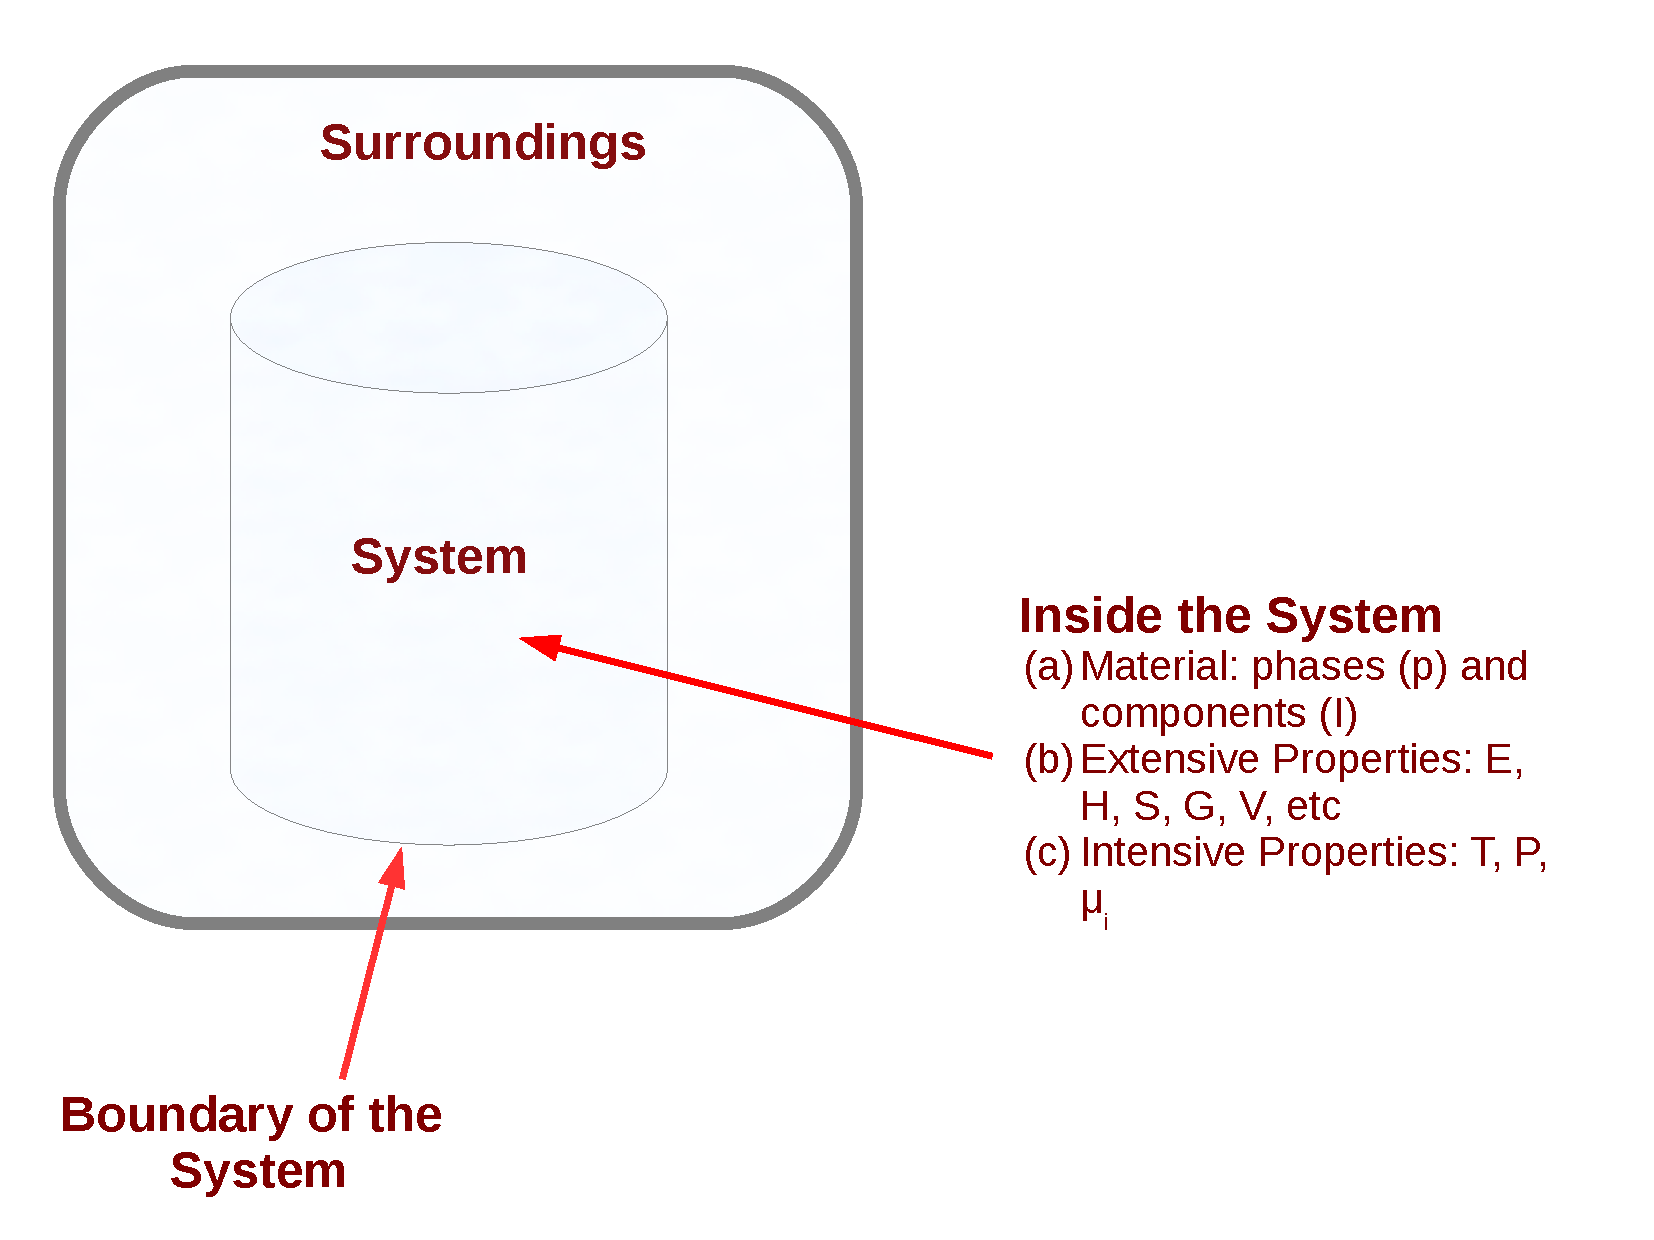
\includegraphics[width=1.05\columnwidth,clip]{./Pics/Fig_SystemDefinition}
        \end{center}
      \end{figure}
      \begin{tabular}{|c|c|c|}
         \hline
                      & {\bf Mass} & {\bf Energy} \\
                      & {\bf Exchange} & {\bf Exchange} \\
         \hline
         {\bf Open}   & {\it yes}  & {\it yes}    \\
         {\bf Closed} & {\it no}   & {\it yes}    \\
         {\bf Isolated}&{\it no}   & {\it no}     \\
         \hline 
      \end{tabular}    
    \end{column}
  \end{columns}
\end{frame}
\normalsize



%%%
%%% Slide
%%%
\scriptsize
\begin{frame}
 \frametitle{System and Control Volumes}
  \begin{columns}
    \begin{column}[l]{0.55\linewidth}
      \begin{itemize}%\scriptsize
       \item <1-> A \textcolor{red}{closed system} (also known as a \textcolor{red}{control mass}) consists of a fixed amount of mass, and no mass can cross its boundary. However, energy (in the form of heat or work) may cross the boundary -- and the volume of a closed system does not have to be fixed; 
       \item <2-> When neither energy nor mass is allowed to cross the boundary, that system is called an \textcolor{red}{isolated system};
       \item <3-> An open system (or \textcolor{red}{control volume}) is a properly selected region in space. It usually encloses a device that involves mass flow such as a compressor, turbine, or nozzle.
      \end{itemize}
    \end{column}
    \begin{column}[l]{0.45\linewidth}\scriptsize
      \begin{figure}%
        \begin{center}
          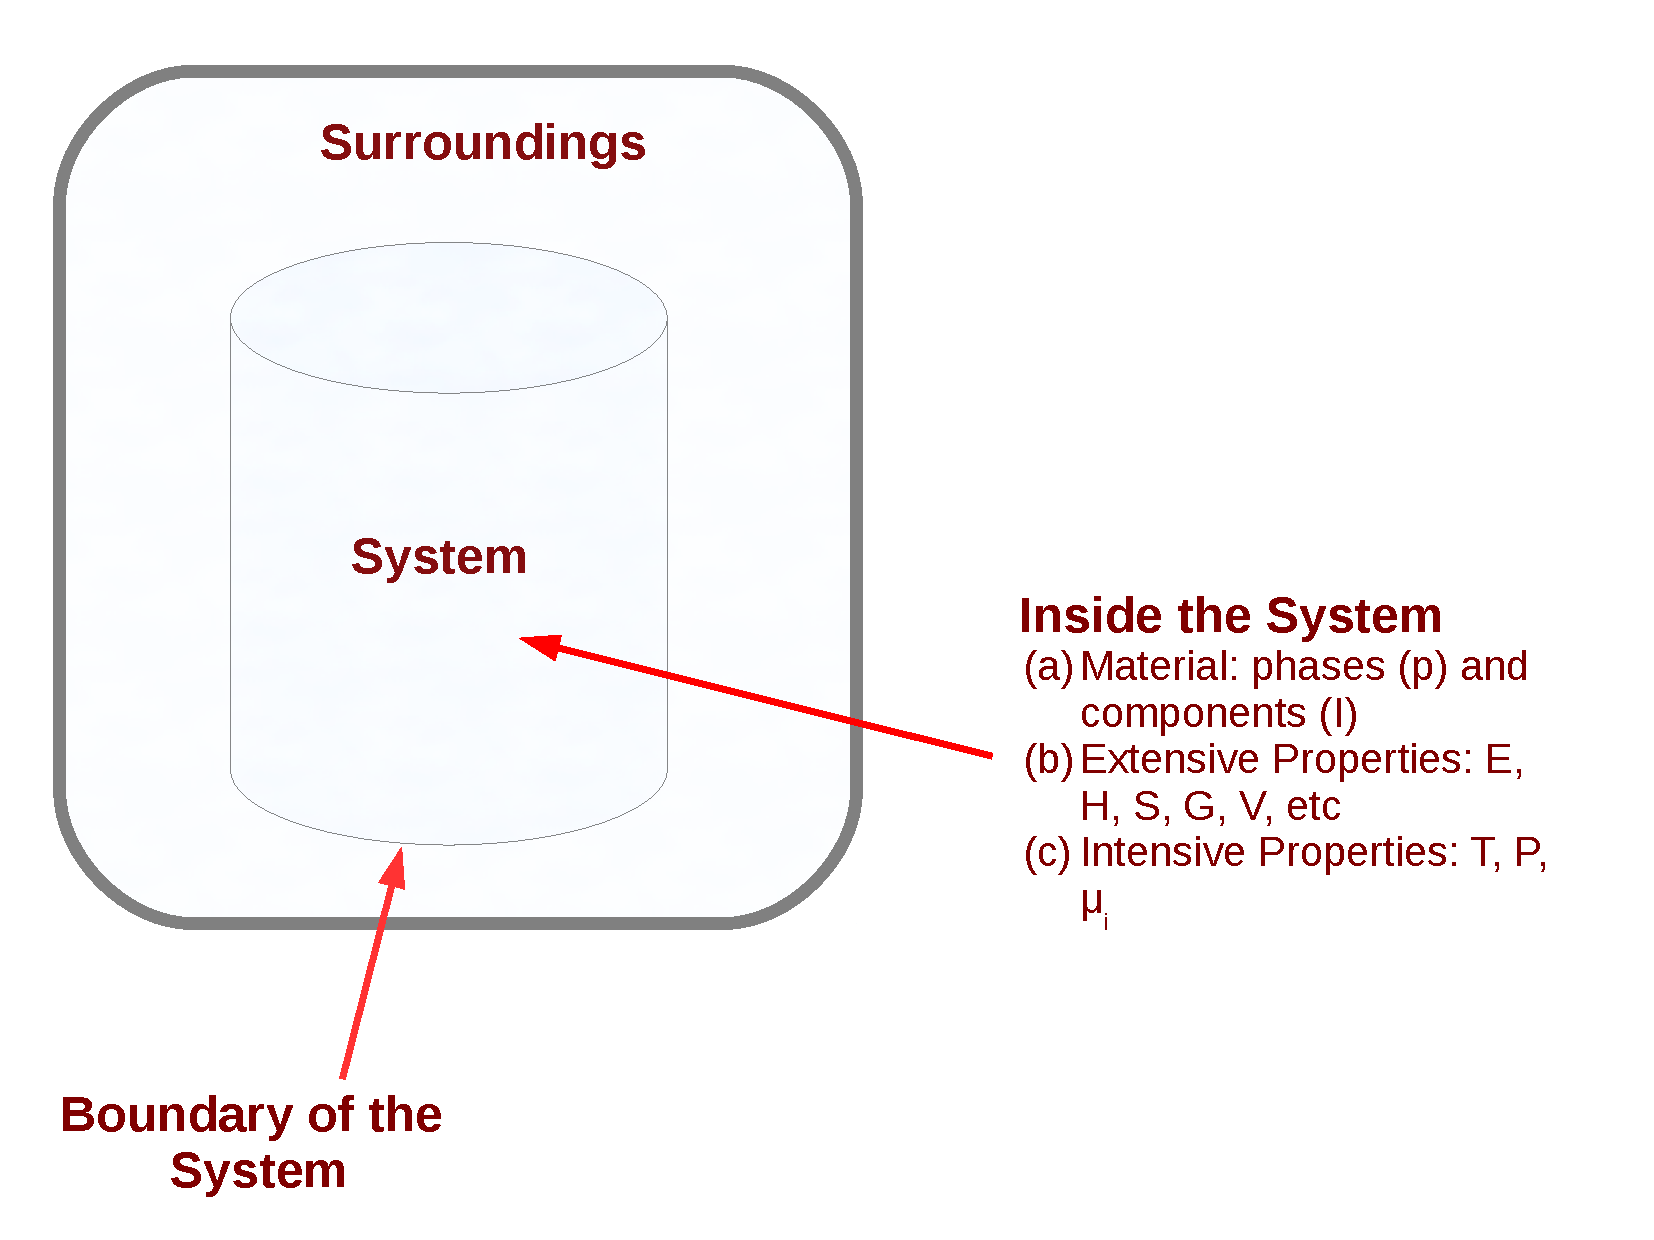
\includegraphics[width=1.05\columnwidth,clip]{./Pics/Fig_SystemDefinition}
        \end{center}
      \end{figure}
      \begin{tabular}{|c|c|c|}
         \hline
                      & {\bf Mass} & {\bf Energy} \\
                      & {\bf Exchange} & {\bf Exchange} \\
         \hline
         {\bf Open}   & {\it yes}  & {\it yes}    \\
         {\bf Closed} & {\it no}   & {\it yes}    \\
         {\bf Isolated}&{\it no}   & {\it no}     \\
         \hline 
      \end{tabular}    
    \end{column}
  \end{columns}
\end{frame}
\normalsize


%%%
%%% Slide
%%%
\begin{frame}
 \frametitle{System and Control Volumes}
 \begin{itemize}
  \item <2-> The \textcolor{red}{material} in a system is composed of phases (e.g., solid, liquid, gas) with distinct physical and chemical properties;
  \item <3-> The \textcolor{red}{composition} of each phase is described by a series of discrete chemical formula units (i.e., chemical components) -- e.g., water/steam $\left(\right.$H$_{2}$O$\left.\right)$, ammonia $\left(\right.$NH$_{3}\left.\right)$, carbon dioxide $\left(\right.$CO$_{2}\left.\right)$, etc;
  \item <4-> Any characteristic of a system is called a \textcolor{red}{property} -- e.g., pressure, temperature, mass, etc;
  \item <5-> Properties can be classified as \textcolor{red}{intensive} or \textcolor{red}{extensive};
  \item <6-> \textcolor{red}{Intensive properties} are those that are {\bf independent} of the mass of a system -- e.g., temperature, pressure, density, viscosity, etc;
  \item <7-> \textcolor{red}{Extensive properties} are those whose values {\bf depend} on the size (or extent) of the system -- e.g., mass, volume, number of moles, internal energy, enthalpy, entropy, etc.  
 \end{itemize}
\end{frame}



\subsection{Review of the Main Thermodynamic Tools}
%%%
%%% Slide
%%%

\begin{frame}
 \frametitle{PVT Behaviour of Pure Substances}
 \begin{columns}
  \begin{column}[l]{0.5\linewidth}
\begin{itemize}
\item <1-> This surface represents the \textcolor{red}{Pressure} - \textcolor{red}{specific volume} - \textcolor{red}{Temperature} -- $PVT$, relation in a pure substance;
\item <2-> Any given coordinate in both, the surface plot and diagrams (projections), will represent values of pressure, specific volume and temperature when the substance is at equilibrium;
\end{itemize}
  \end{column}
  \begin{column}[l]{0.5\linewidth}
   \begin{figure}%
    \begin{center}
     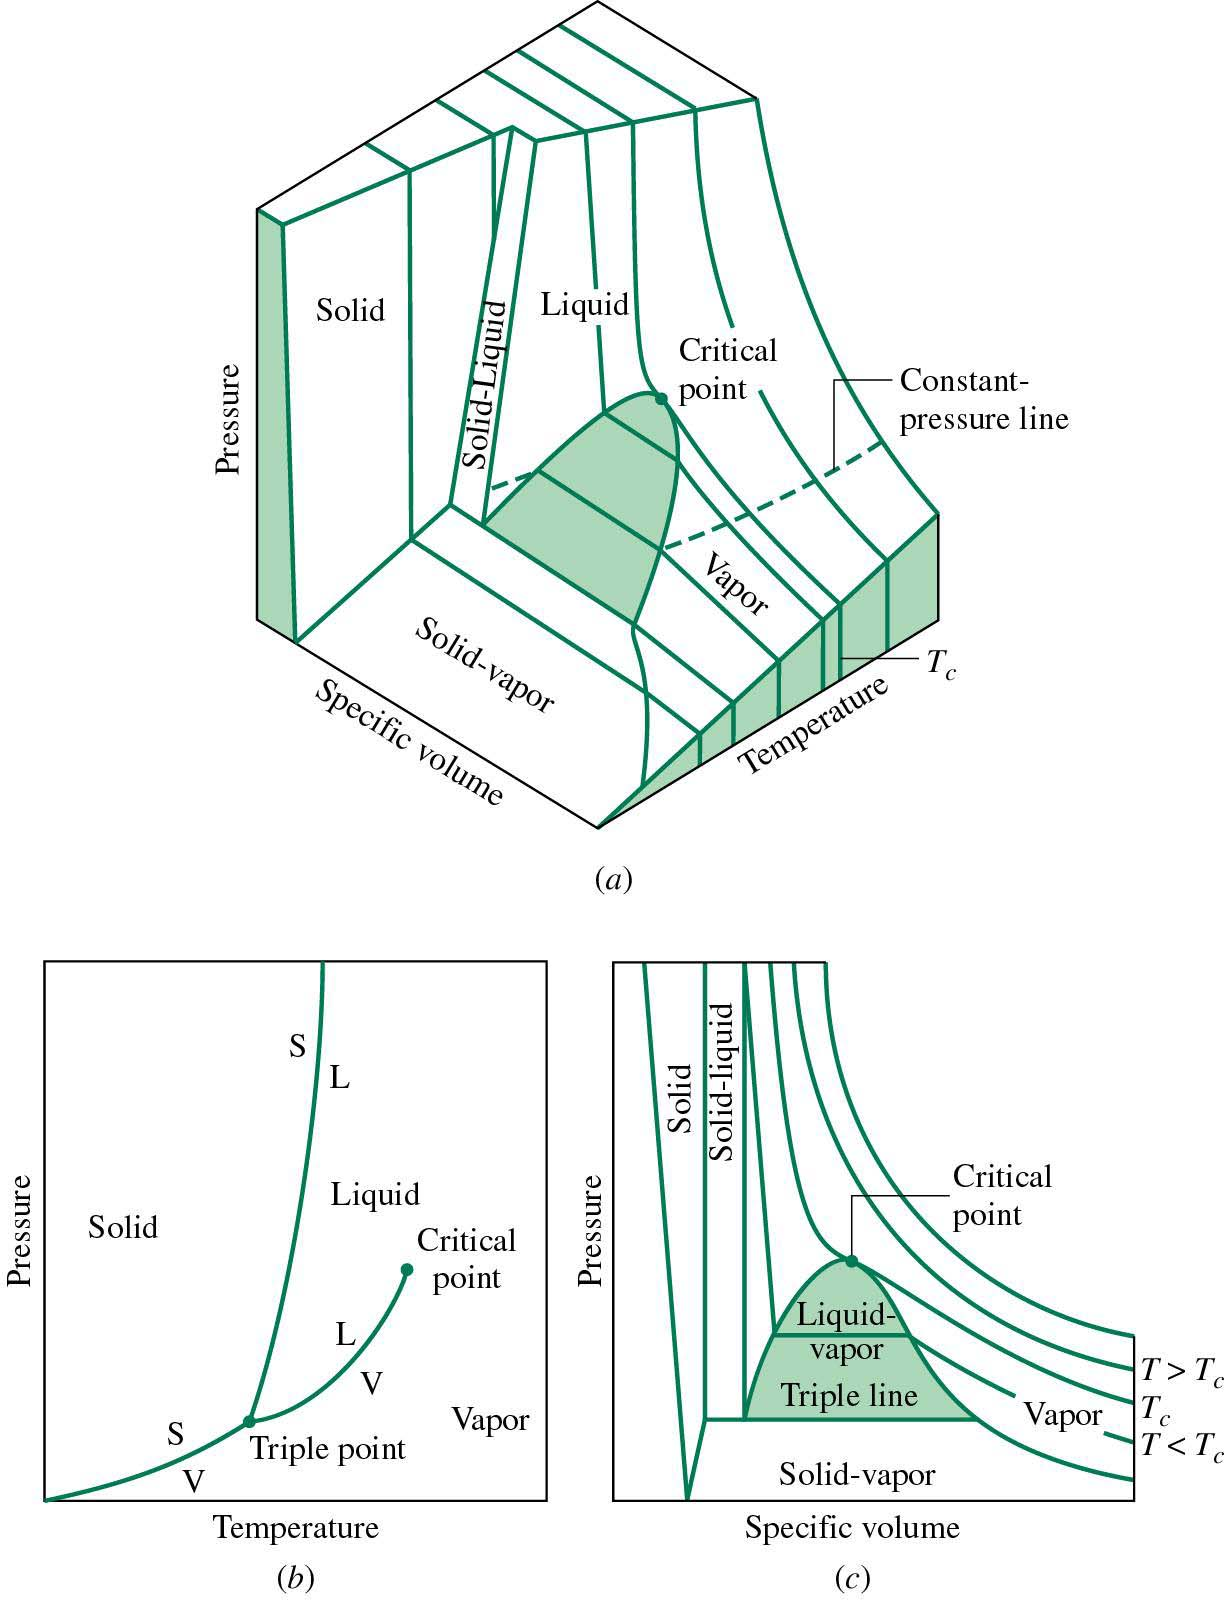
\includegraphics[width=4.cm,clip]{./Pics/PVT_Surface.jpg}
    \end{center}
\caption{$PVT$ surface (top) and projections onto (b) $PT$ and (c) $PV$ diagrams for a pure substance (Extracted from Moran {\it et al.})}
   \end{figure}    
  \end{column}
 \end{columns}
\end{frame}



%%%
%%% Slide
%%%

\begin{frame}
 \frametitle{PVT Behaviour of Pure Substances}
 \begin{columns}
  \begin{column}[l]{0.5\linewidth}
\begin{itemize}
\item <1-> The \textcolor{red}{Gibbs phase rule},
\begin{equation}
\Psi = 2 + \mathcal{C} - \mathcal{P}
\end{equation} 
\item <2-> describes the number of degrees of freedom (dof), $\Psi$ (intensive variables, e.g., temperature, pressure), in a closed system at equilibrium as a function of the number of phases ($\mathcal{P}$ = solid, liquid and vapour) and components, $\mathcal{C}$ (e.g., water, CO$_{2}$, N$_{2}$, etc). 
\end{itemize}
  \end{column}
  \begin{column}[l]{0.5\linewidth}
   \begin{figure}%
    \begin{center}
     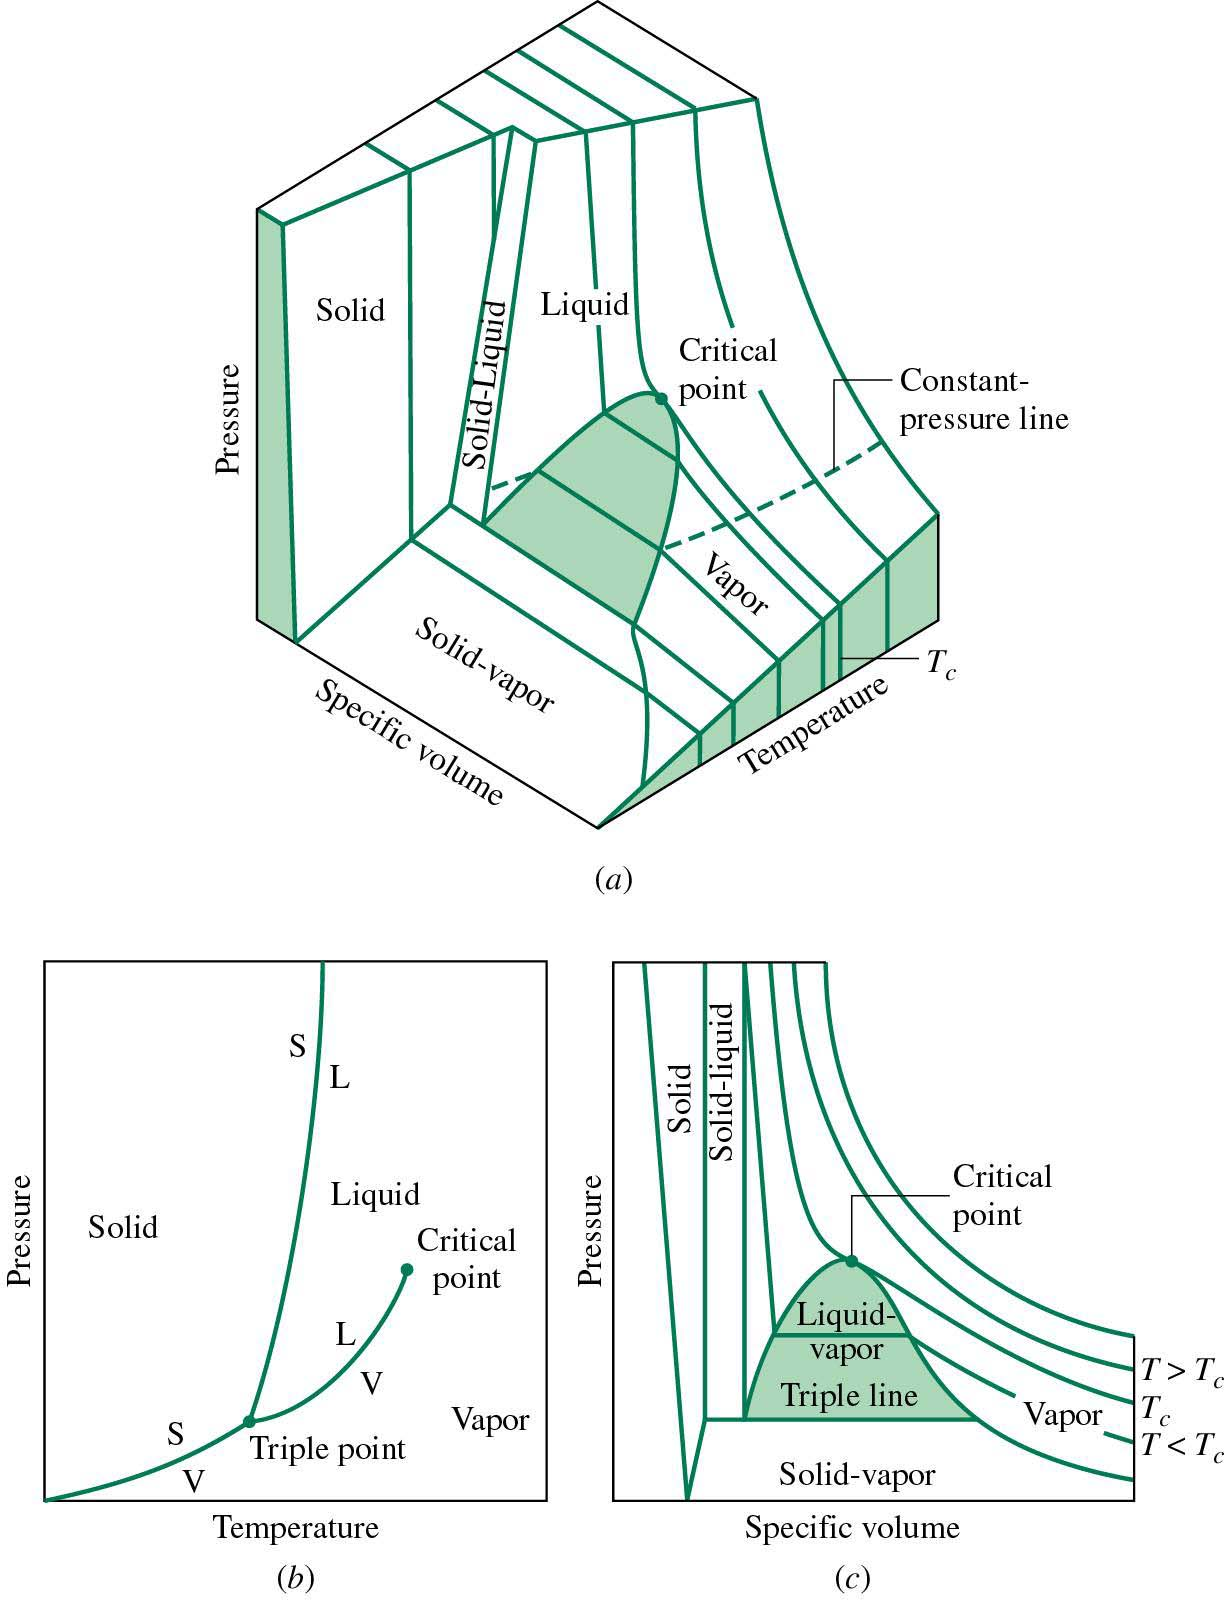
\includegraphics[width=4.cm,clip]{./Pics/PVT_Surface.jpg}
    \end{center}
\caption{$PVT$ surface (top) and projections onto (b) $PT$ and (c) $PV$ diagrams for a pure substance (Extracted from Moran {\it et al.})}
   \end{figure}    
  \end{column}
 \end{columns}
\end{frame}


%%%
%%% Slide
%%%

\begin{frame}
 \frametitle{PVT Behaviour of Pure Substances}
 \begin{columns}
  \begin{column}[l]{0.55\linewidth}
\begin{itemize}
\item <1-> {\bf Example:} In the $PT$ diagram (b) for one hypothetical component -- $\textcolor{red}{\mathcal{C}=1}$, within each phase region -- $\textcolor{blue}{\mathcal{P}=1}$ (i.e., as either solid, liquid or vapour phases),
\begin{displaymath}
\Psi = 2 + \textcolor{red}{1} - \textcolor{blue}{1} = 2
\end{displaymath}
\item <2-> In this case, the number of degrees of freedom correspond to temperature and pressure;
\item <3-> Thus, within (e.g.) the vapour phase, temperature and pressure can readily be changed without explicit phase change or composition of the vapour phase.
\end{itemize}
  \end{column}
  \begin{column}[l]{0.45\linewidth}
   \begin{figure}%
    \begin{center}
     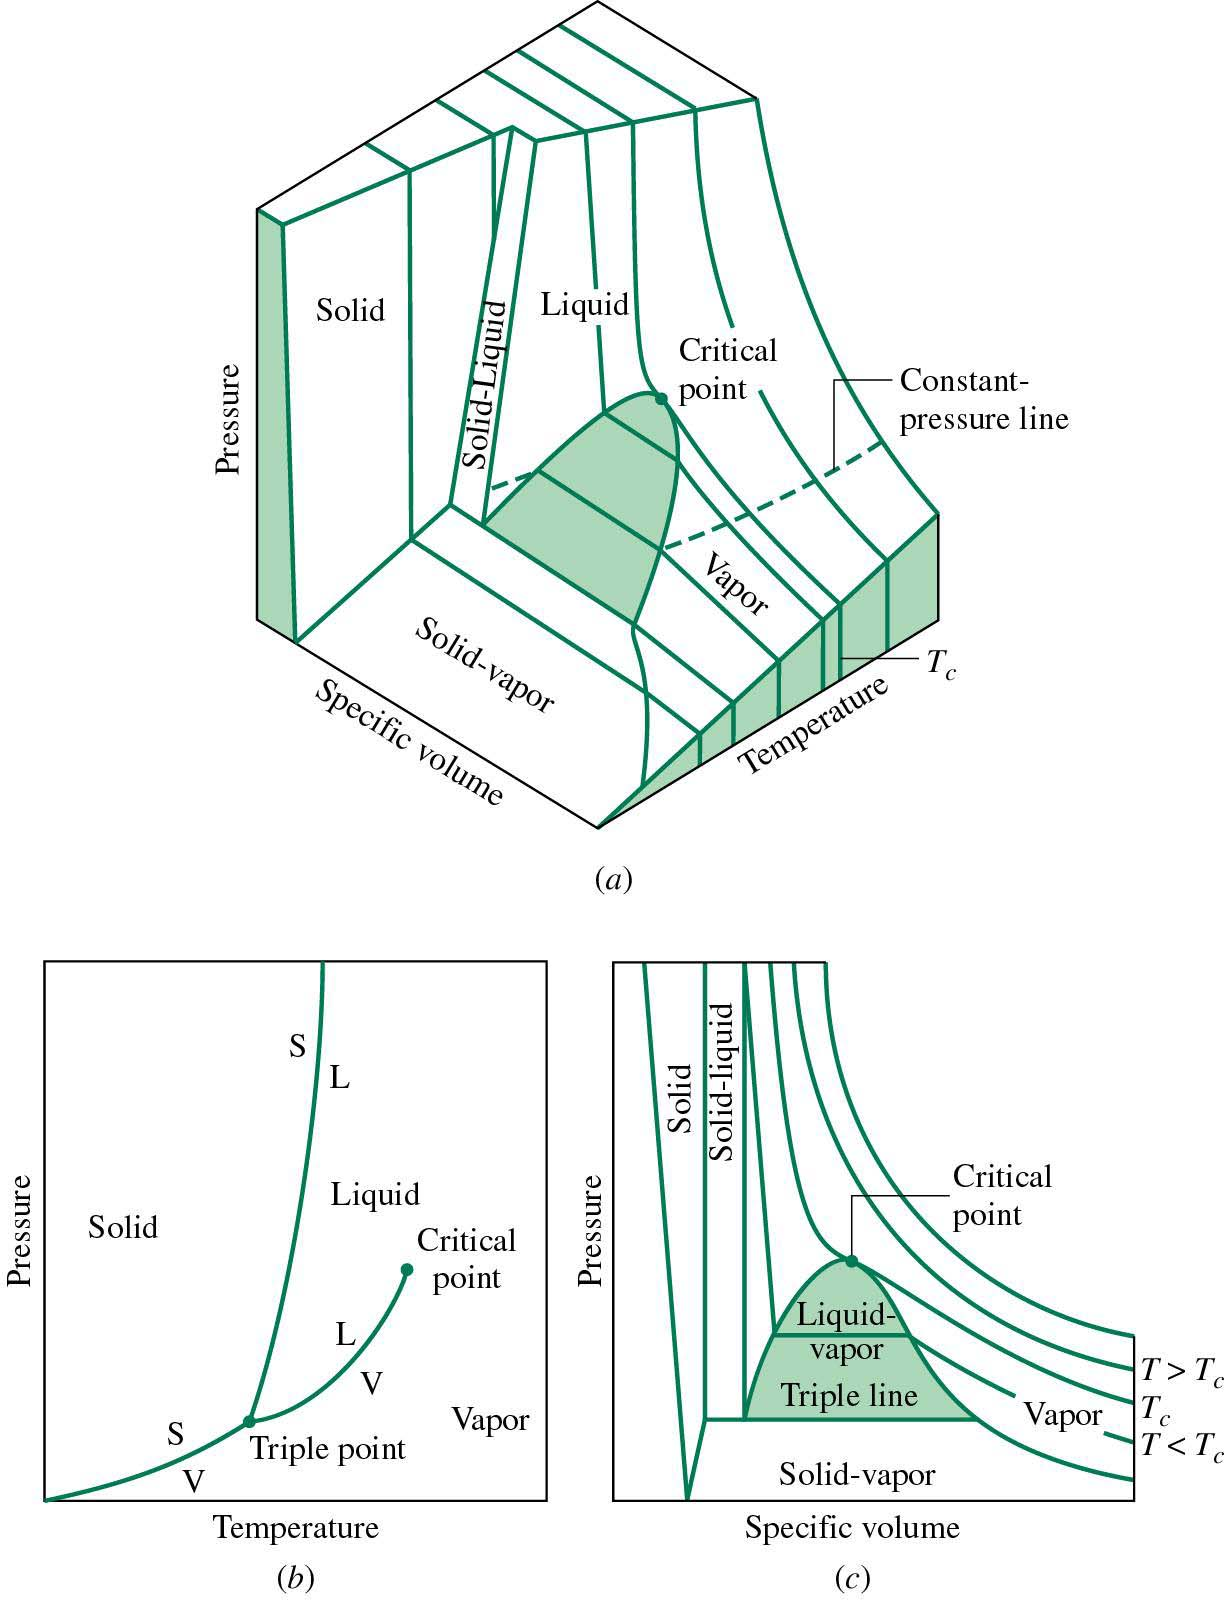
\includegraphics[width=4.cm,clip]{./Pics/PVT_Surface.jpg}
    \end{center}
\caption{$PVT$ surface (top) and projections onto (b) $PT$ and (c) $PV$ diagrams for a pure substance (Extracted from Moran {\it et al.})}
   \end{figure}    
  \end{column}
 \end{columns}
\end{frame}


%%%
%%% Slide
%%%

\begin{frame}
 \frametitle{PVT Behaviour of Pure Substances}
 \begin{columns}
  \begin{column}[l]{0.5\linewidth}
\begin{itemize}
\item <1-> However, along with the \textcolor{red}{phase-line boundary}, two phases are in equilibrium, i.e., $\textcolor{blue}{\mathcal{P}=2}$,%
\begin{displaymath}
\Psi = 2 + \textcolor{red}{1} - \textcolor{blue}{2} = 1
\end{displaymath}
\item <2-> When the vapour and liquid phases are in equilibrium, any change in temperature {\bf leads} to change in pressure for the system remains in equilibrium;
\end{itemize}
  \end{column}
  \begin{column}[l]{0.5\linewidth}
   \begin{figure}%
    \begin{center}
     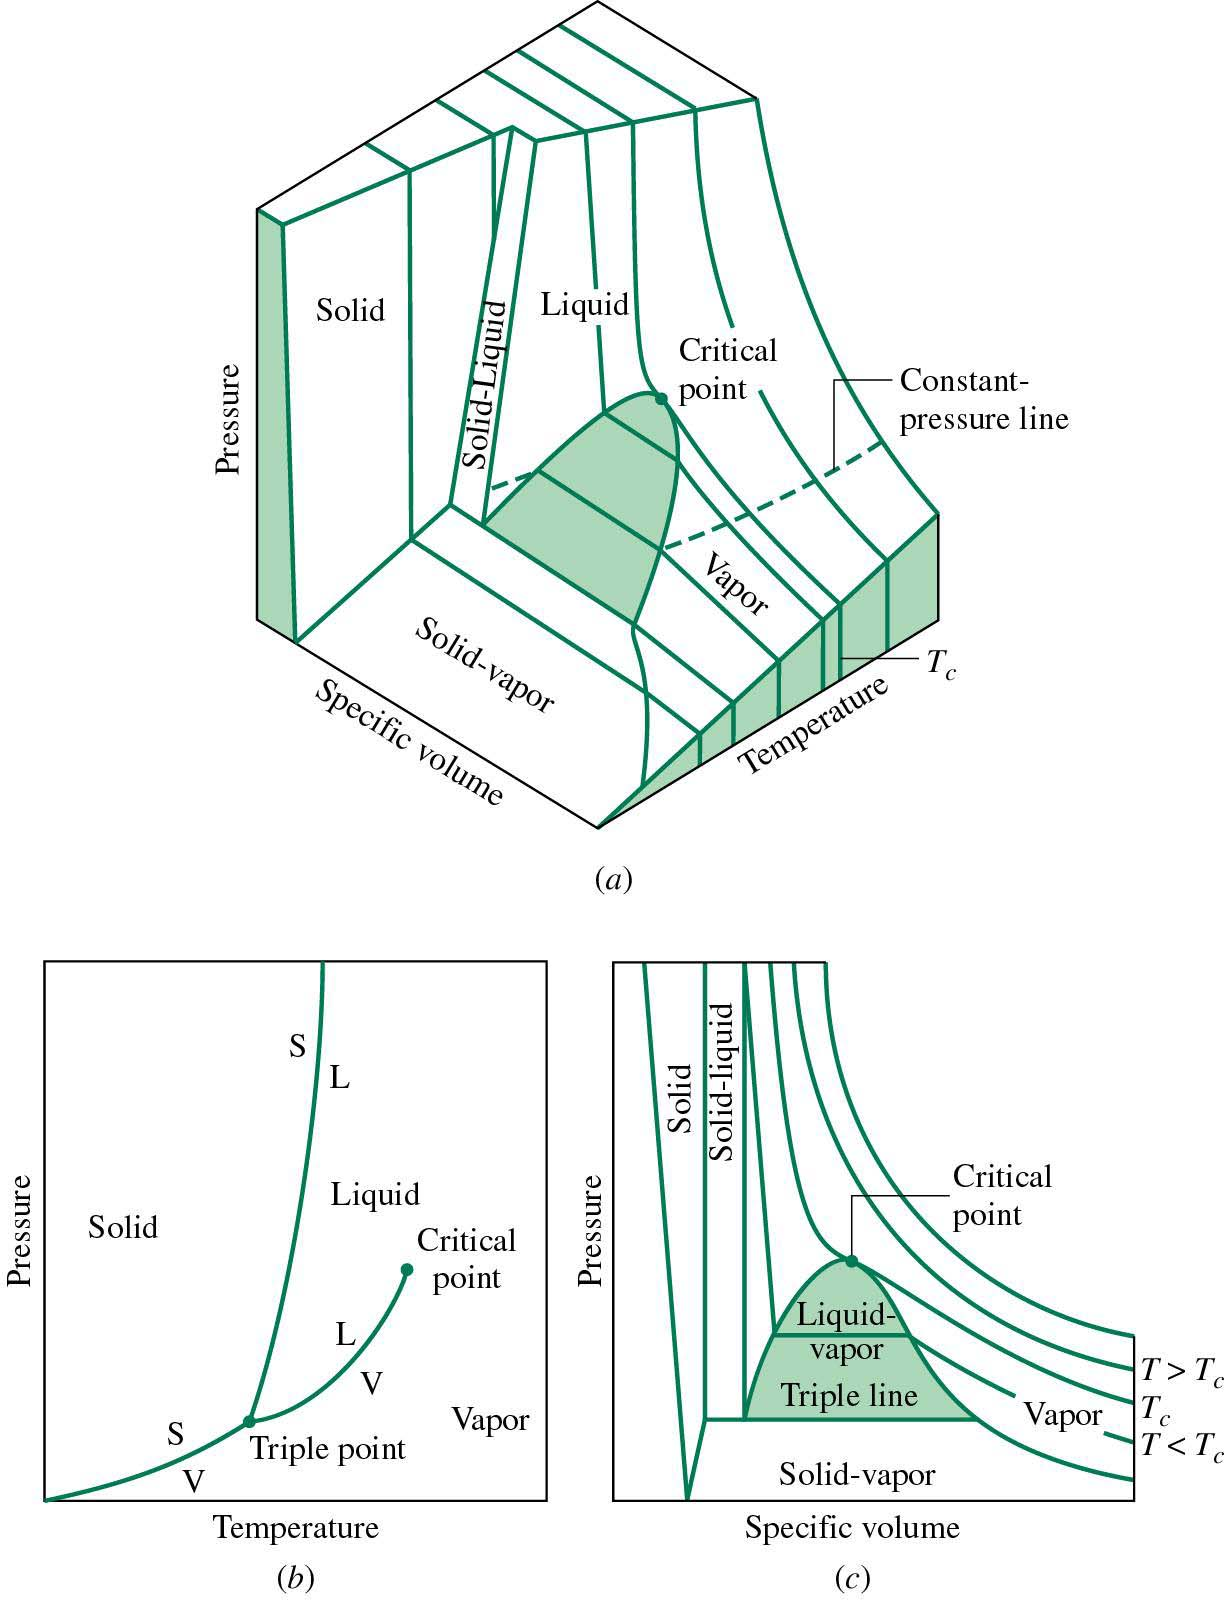
\includegraphics[width=4.cm,clip]{./Pics/PVT_Surface.jpg}
    \end{center}
\caption{$PVT$ surface (top) and projections onto (b) $PT$ and (c) $PV$ diagrams for a pure substance (Extracted from Moran {\it et al.})}
   \end{figure}    
  \end{column}
 \end{columns}
\end{frame}


%%%
%%% Slide
%%%

\begin{frame}
 \frametitle{PVT Behaviour of Pure Substances}
 \begin{columns}
  \begin{column}[l]{0.5\linewidth}
\begin{itemize}
\item <1-> Similarly, for the {\bf triple point} -- $\textcolor{blue}{\mathcal{P}=3}$, all three phases are in equilibrium
\begin{displaymath}
\Psi = 2 + \textcolor{red}{1} - \textcolor{blue}{3} = 0
\end{displaymath}
\item <2-> Here there is {\bf no degrees of freedom} -- i.e., there is {\bf just} one value for pressure and temperature that make the {\bf three phases to coexist}.
\item <3-> Any change in either intensive properties will drive the system away from the {\it triple point}.
\end{itemize}
  \end{column}
  \begin{column}[l]{0.5\linewidth}
   \begin{figure}%
    \begin{center}
     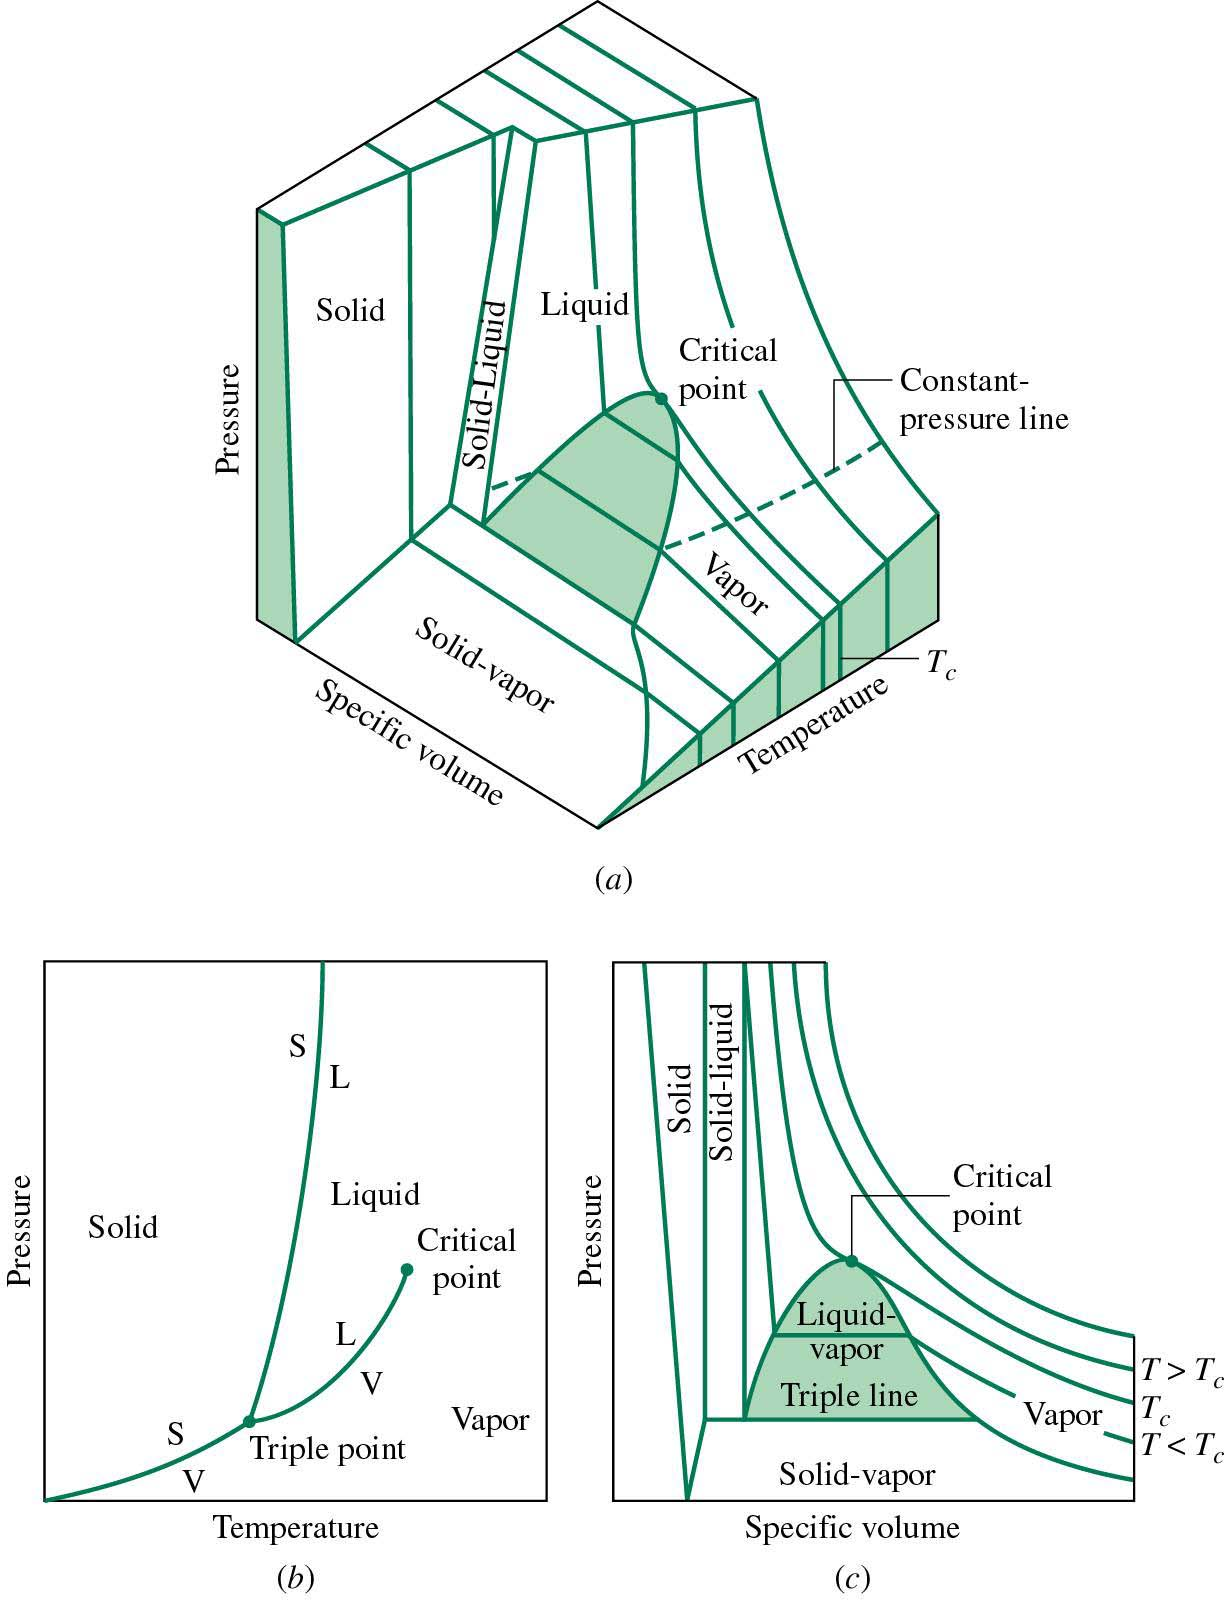
\includegraphics[width=4.cm,clip]{./Pics/PVT_Surface.jpg}
    \end{center}
\caption{$PVT$ surface (top) and projections onto (b) $PT$ and (c) $PV$ diagrams for a pure substance (Extracted from Moran {\it et al.})}
   \end{figure}    
  \end{column}
 \end{columns}
\end{frame}



%%%
%%% SUBSECTION
%%%
\subsection{Thermodynamic Diagrams and Tables}

%%%
%%% Slide
%%%
\begin{frame}
 \frametitle{Thermodynamics Diagrams: Pressure $\times$ Enthalpy $(PH)$ for CO$_{2}$}
  \begin{center}
   \begin{figure}
     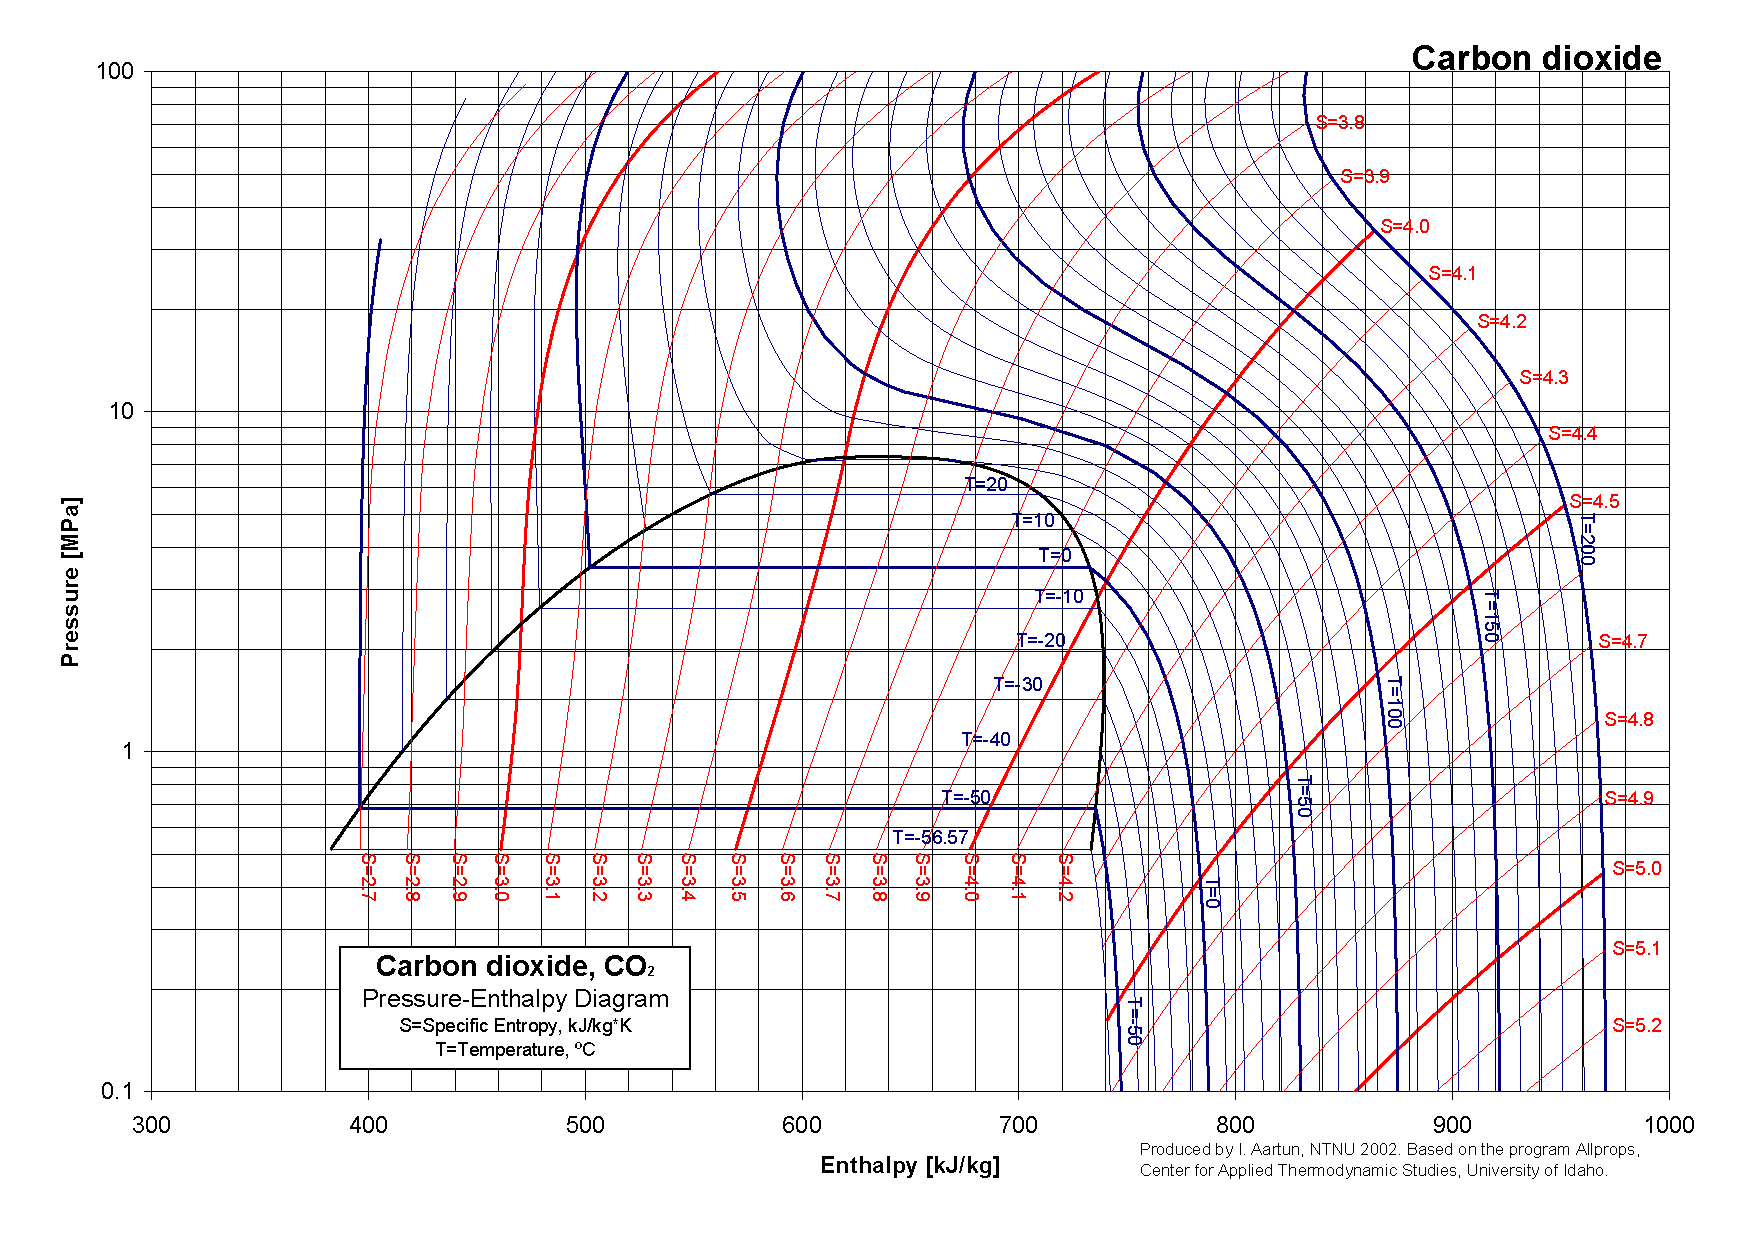
\includegraphics[width=8cm,height=7.cm,clip]{./Pics/CO2col}
   \end{figure}
   \end{center}
\end{frame}

%%%
%%% Slide
%%%
\begin{frame}
 \frametitle{Thermodynamics Diagrams: Pressure $\times$ Enthalpy $(PH)$}
  \begin{center}
   \begin{figure}
      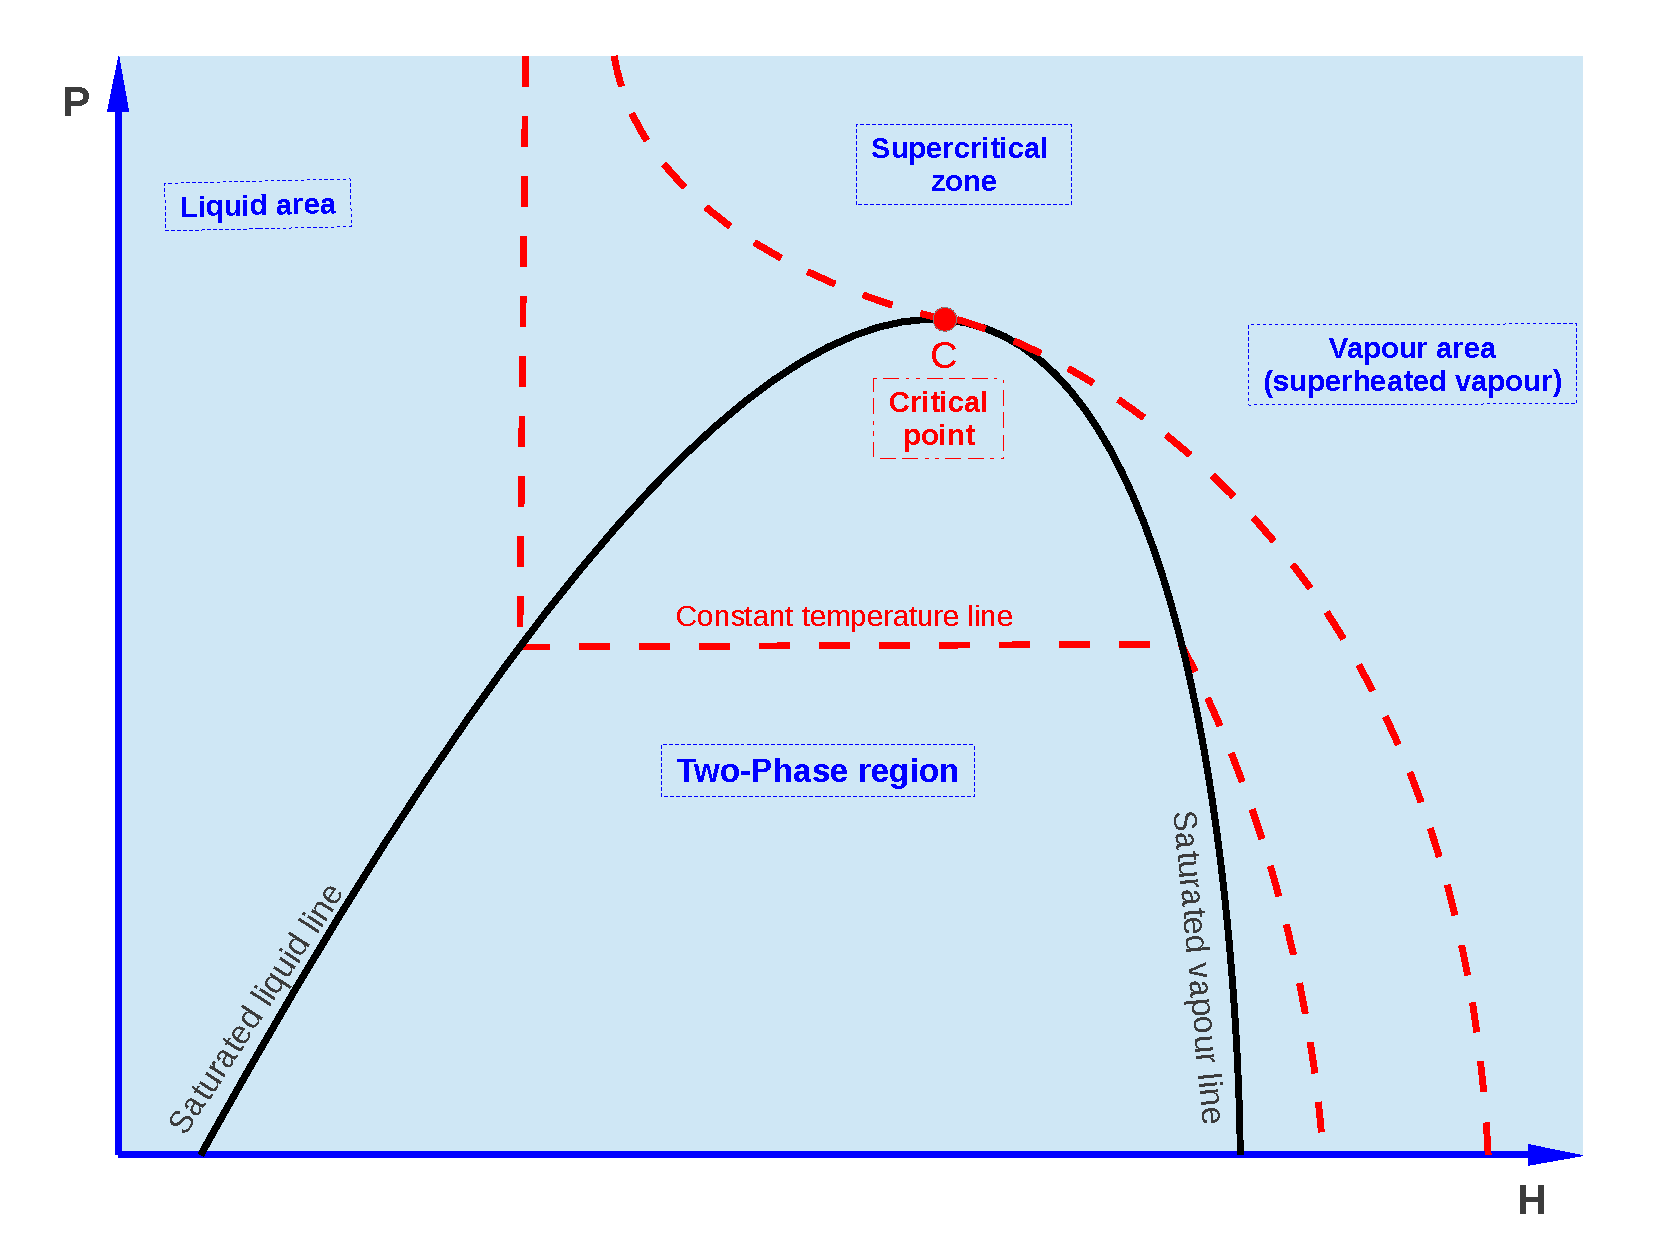
\includegraphics[width=8cm,height=7.9cm,clip]{./Pics/Overview_Refrig18}
   \end{figure}
   \end{center}
\end{frame}

%%%
%%% Slide
%%%
\begin{frame}
 \frametitle{Thermodynamics Diagrams: Pressure $\times$ Enthalpy $(PH)$}
  \begin{center}
   \begin{figure} 
      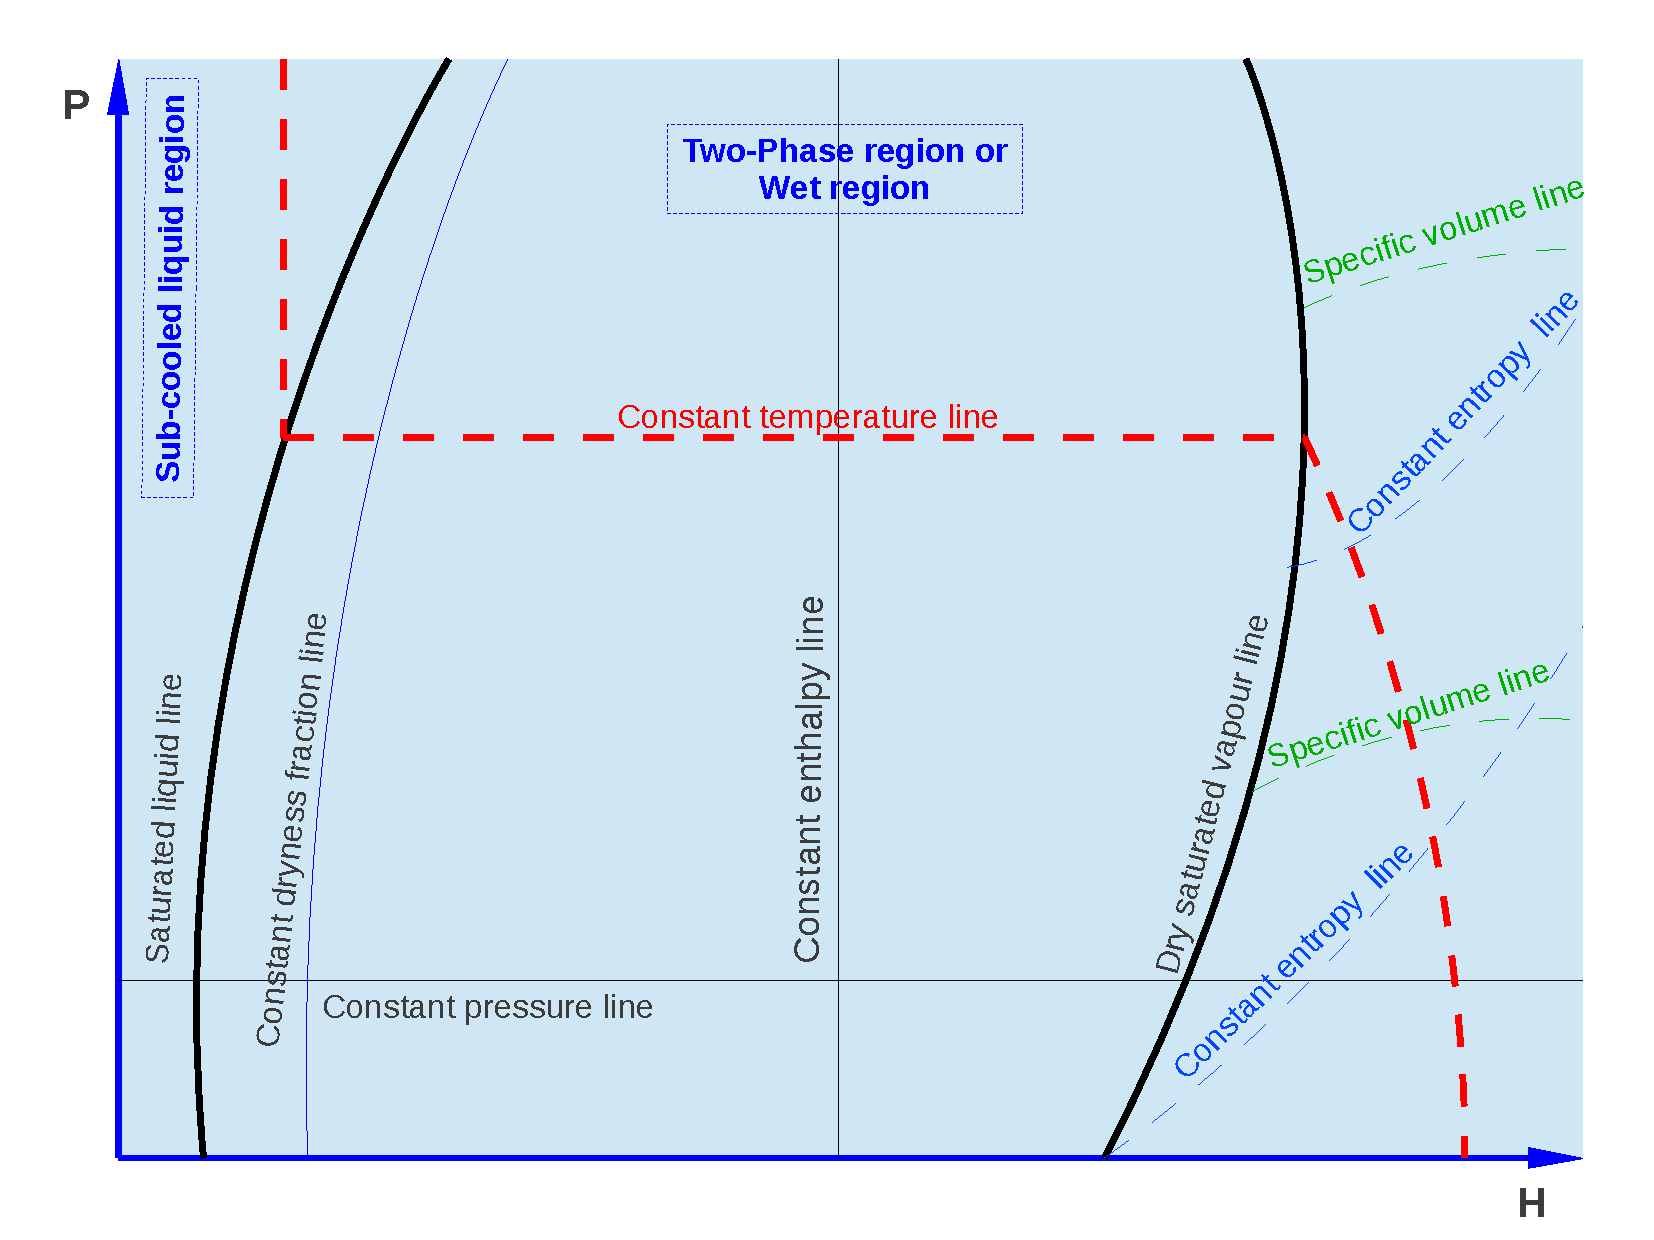
\includegraphics[width=8cm,height=7.9cm,clip]{./Pics/Overview_Refrig17}
   \end{figure}
   \end{center}
\end{frame}

%%%
%%% Slide
%%%
\begin{frame}
 \frametitle{Thermodynamics Diagrams: Temperature $\times$ Entropy $(TS)$ for Water}
  \begin{center}
   \begin{figure}
     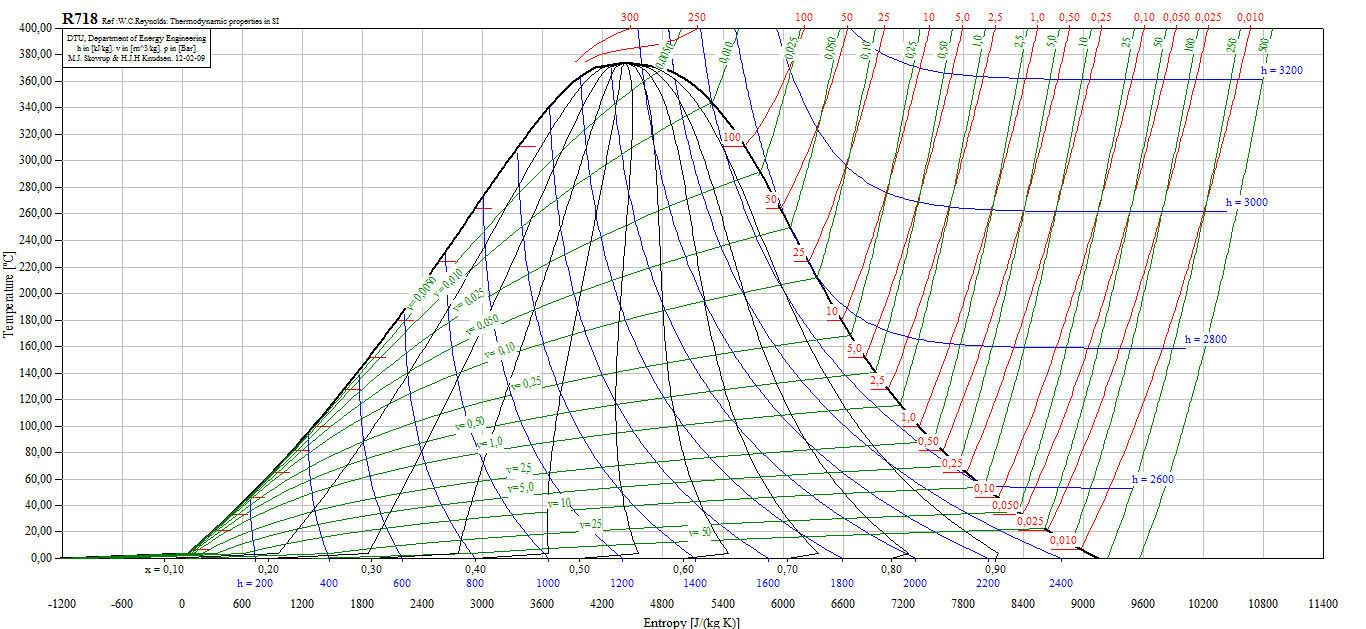
\includegraphics[width=8cm,height=7.cm,clip]{./Pics/water_TS.png}
   \end{figure}
   \end{center}
\end{frame}

%%%
%%% Slide
%%%
\begin{frame}
 \frametitle{Thermodynamics Diagrams: Temperature $\times$ Entropy $(TS)$}
  \begin{center}
   \begin{figure}
      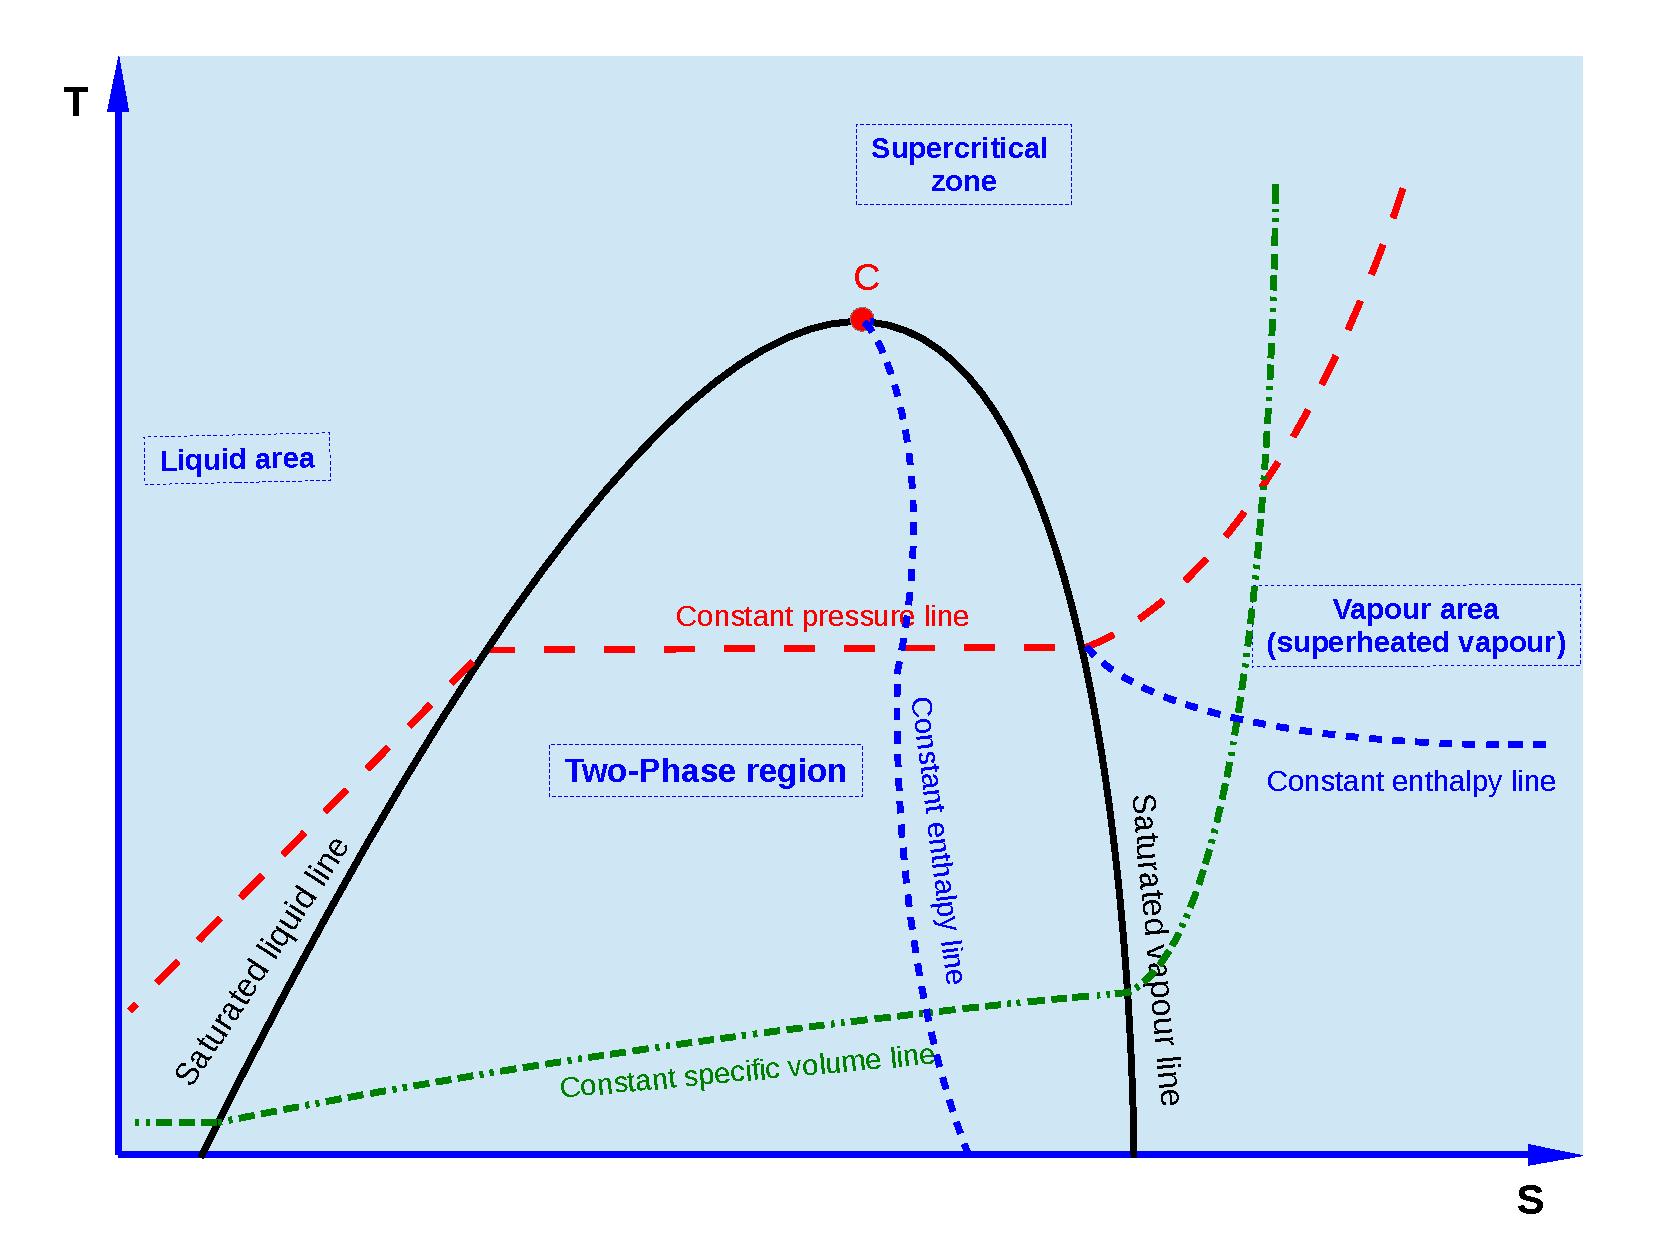
\includegraphics[width=8cm,height=7.9cm,clip]{./Pics/TS_Diag_Schematics}
   \end{figure}
   \end{center}
\end{frame}

%%% 
%%% Slide
%%%
\begin{frame}
  \frametitle{Another option: (a) Saturated Tables and ...}
\scriptsize{From Reference (d):}\vspace{-.8cm}
   \begin{center}
   \begin{figure}
      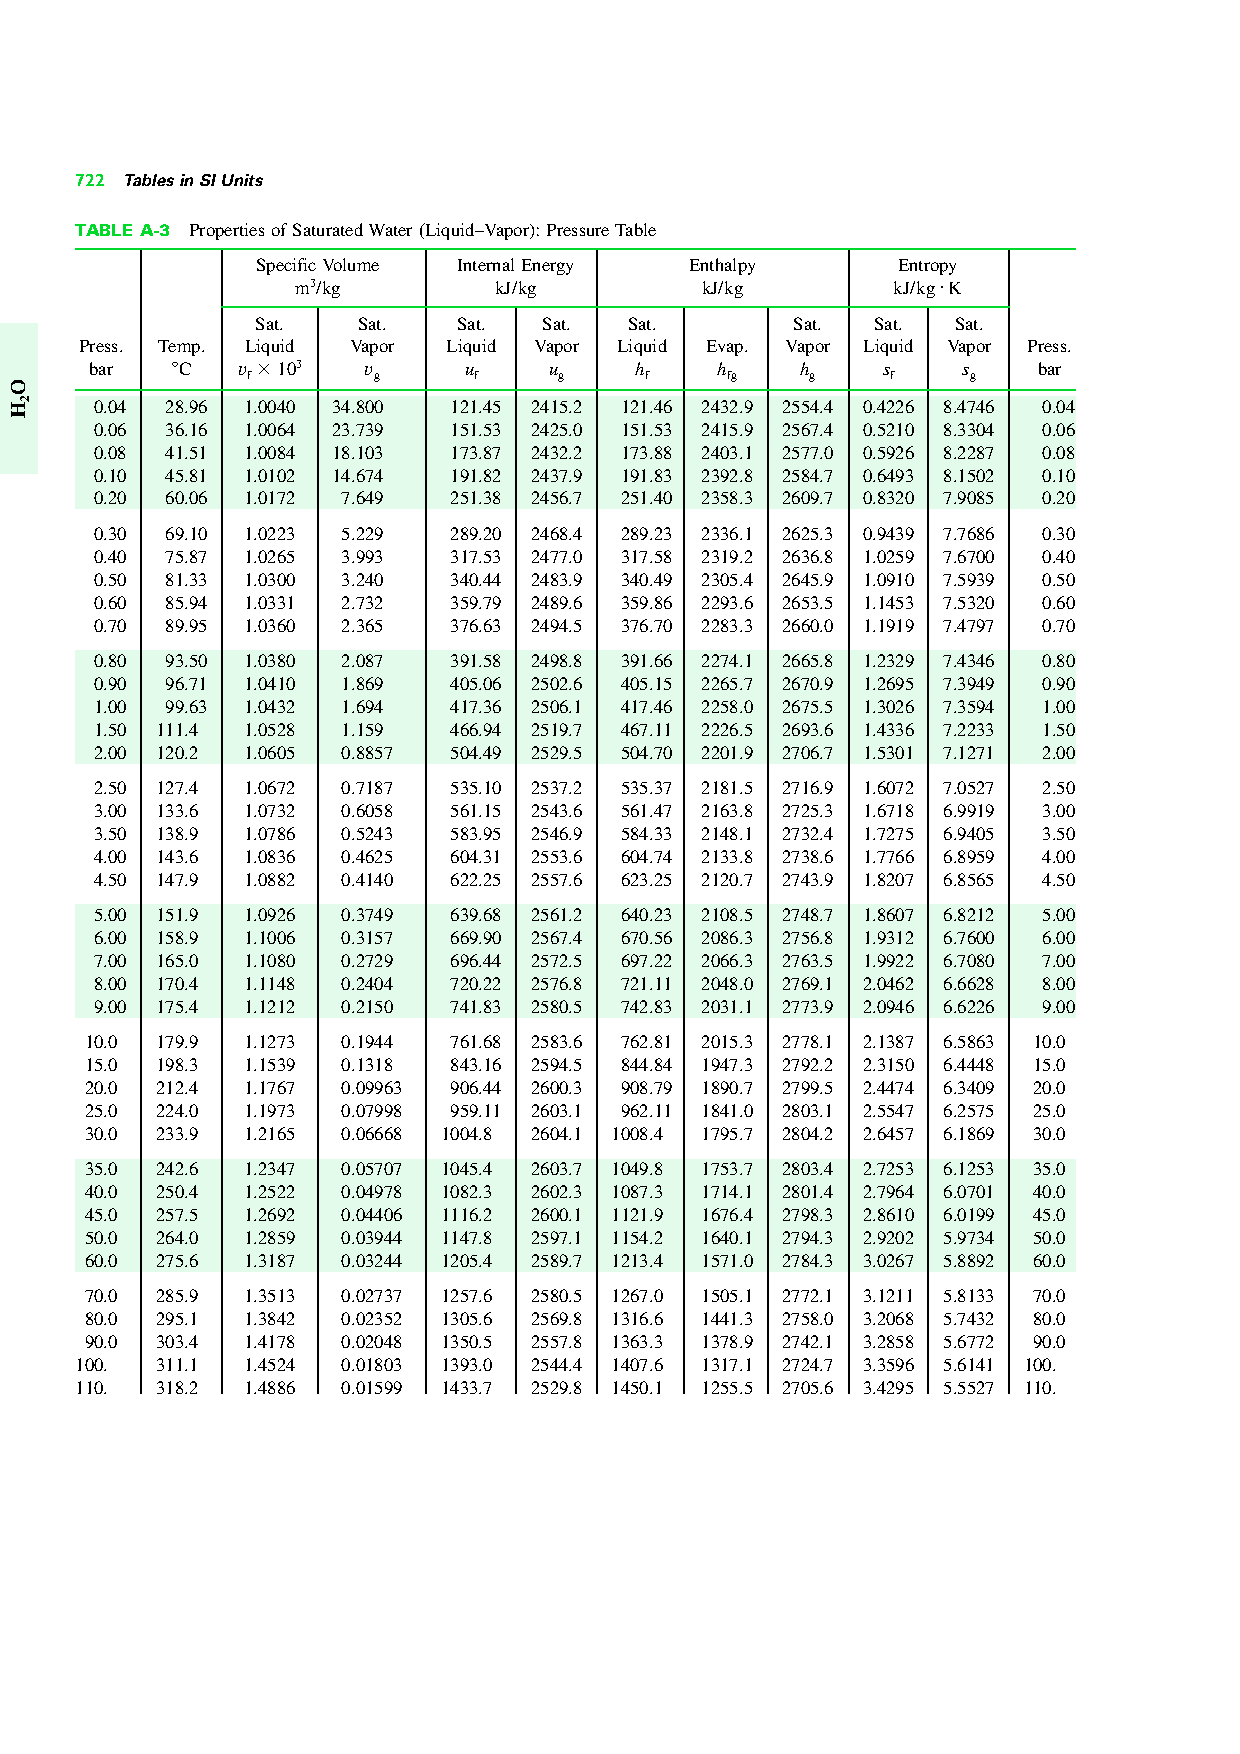
\includegraphics[width=9.5cm,height=9.5cm,clip]{./Pics/WaterSatTable}
   \end{figure}
   \end{center}
\end{frame}


%%%
%%% Slide
%%%
\begin{frame}
  \frametitle{Another option: (b) Superheated Tables}
\scriptsize{From Reference (d):}\vspace{-.8cm}
   \begin{center}
   \begin{figure}
      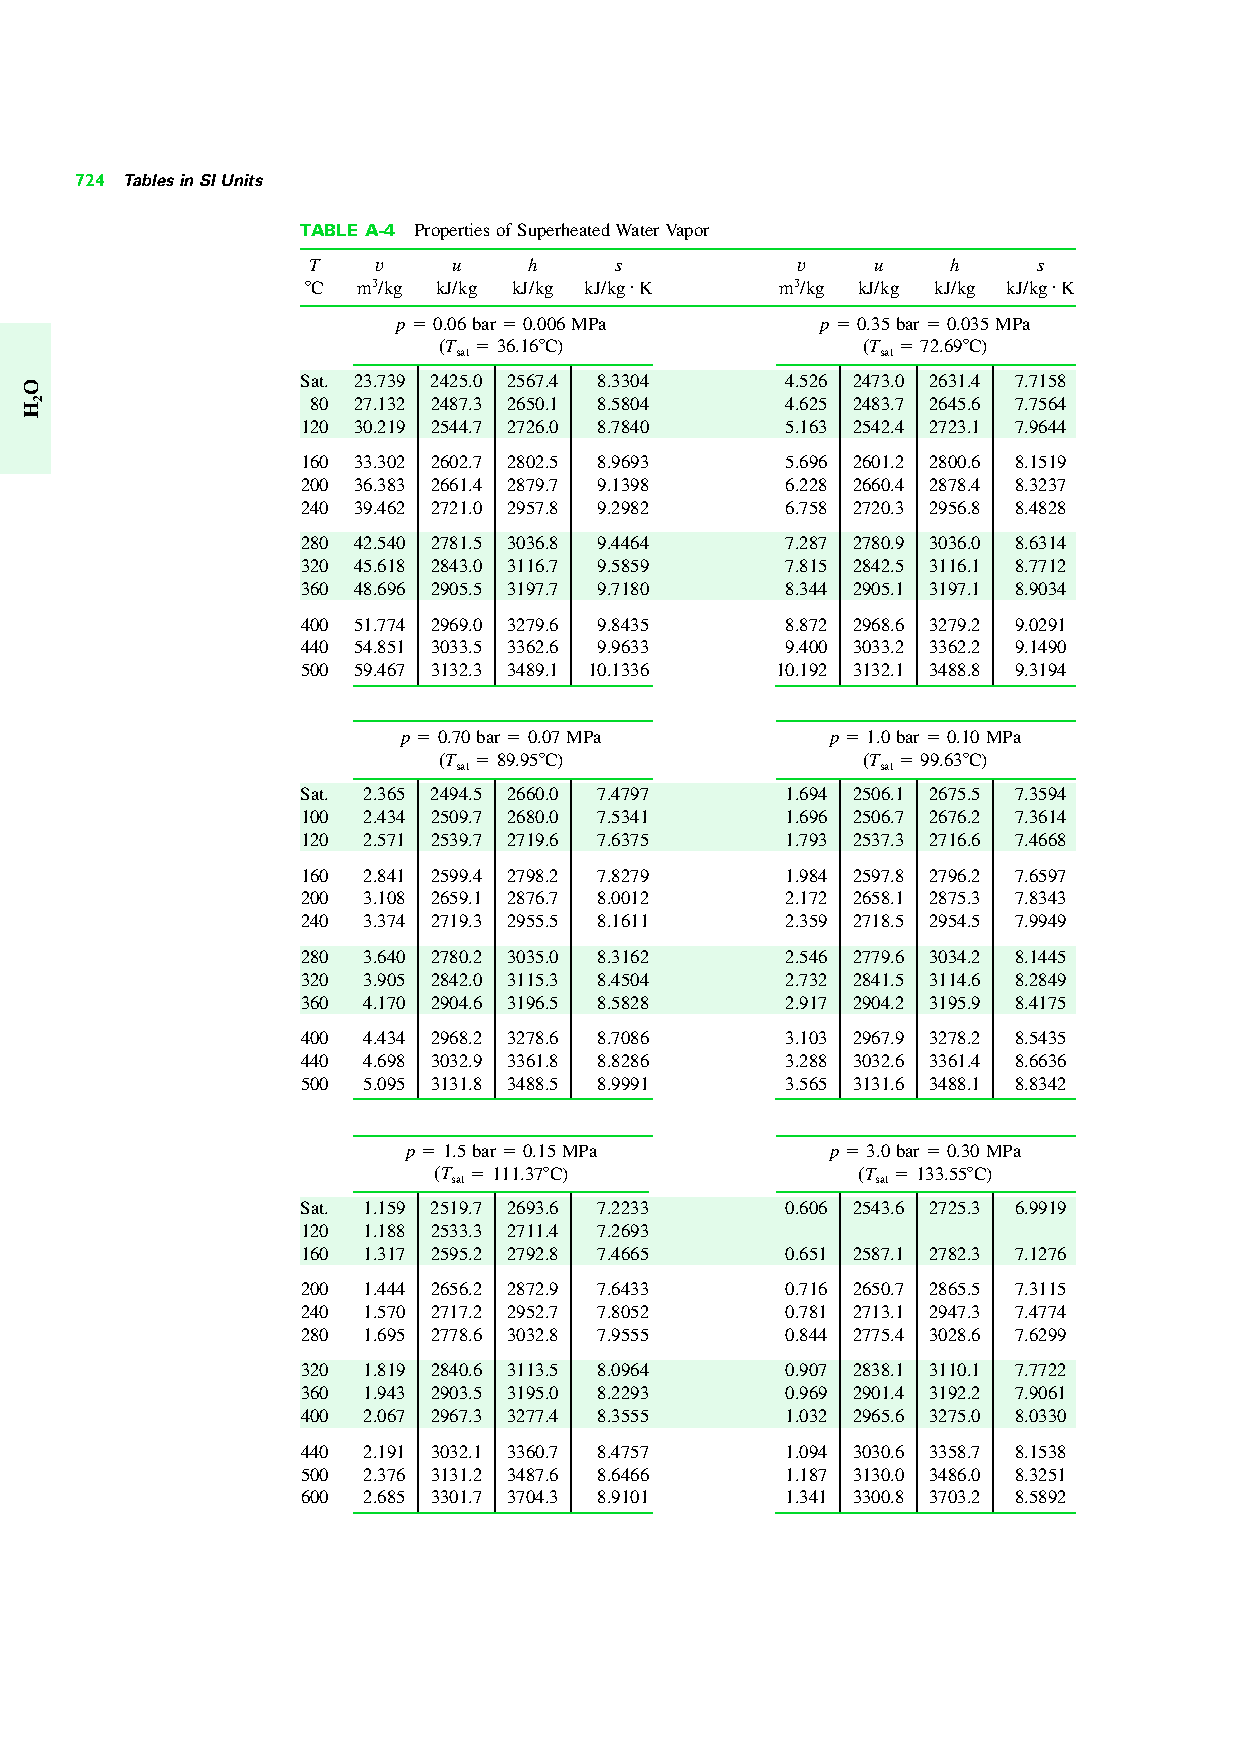
\includegraphics[width=9.5cm,height=9.5cm,clip]{./Pics/Water_SuperheatedTable}
   \end{figure}
   \end{center}
\end{frame}


%%%
%%% Slide
%%%
\begin{frame}
  \frametitle{Another option: Saturated and Superheated Tables}
\noindent
\begin{itemize}
\item <1-> {\bf \textcolor{red}{Example:}} At $P=1.50\;$ bar, the saturated steam has the following thermodynamic properties,
\tiny 
\begin{center}
%\begin{table}[h]
\begin{tabular}{c c|c c c|c c|c c} 
%\hline\hline
$P$ & $T$ & $h_{f}$ &  $h_{fg}$ & $h_{g}$ & $s_{f}$ &  $s_{g}$ & $v_{f}$ & $v_{g}$ \\ 
\hline
1.50 & 111.4 & 467.11 & 2226.5 & 2693.6 & 1.4336 & 7.2233 & 0.0010528 & 1.159 \\
%\hline
\end{tabular}
%\caption{Carnot and Rankine Cycles: From Saturated water and steam tables.}
%\label{Example01_01:Table2}
%\end{table}
\end{center}

\item <3-> But the properties of superheated steam at the same pressure will depend on the temperature $\Rightarrow$ \textcolor{red}{see superheated steam table}. Thus at 1.50 bar $\left(\text{with }T_{\text{sat}}=111.4^{\circ}\text{C}\right)$:
  \visible<3->{\begin{center}\begin{tabular}{ c | c c c}
      $T$    & $v$    & $h$     &    $s$     \\
\hline
      111.4  & 1.159  & 2693.6  &  7.2233    \\
      120.0  & 1.188  & 2711.4  &  7.2693    \\
      160.0  & 1.317  & 2792.8  &  7.4665    \\
      200.0  & 1.444  & 2872.9  &  7.6433    \\
      240.0  & 1.570  & 2952.7  &  7.8052    \\ 
     $\vdots$& $\vdots$&$\vdots$&$\vdots$ \\
  \end{tabular}
  \end{center}
}
\item <2-> {\bf Units:} [$P$] = bar, [$T$] = $^{o}$C, [$h$]= $\frac{kJ}{kg}$, [$s$]=$\frac{kJ}{kg.K}$, [$v$]=$\frac{m^{3}}{kg}$.

\end{itemize}

\end{frame}

%%%
%%% SUBSECTION
%%%
\subsection{Linear Interpolation}
%%%
%%% Slide
%%%
\begin{frame}
  \frametitle{Linear Interpolation}
\noindent
\begin{itemize}
\item <2-> Some of the problems in this course involves extracting values from the thermodynamic tables;
\item <3-> And although the tables are very extensive (for most of the materials), sometimes we need values that can not be directly found on them;
\item <4-> In this case, we just operate a {\bf linear interpolation} between neighbour fields;
\item <5-> For example, water-steam at 1.5 bar and 212$^{o}$C. At this pressure, the {\bf saturation temperature} is 111.3$^{o}$C, therefore we know that the fluid (water/steam) is at \textcolor{red}{superheated state} -- \textcolor{red}{$T > T_{\text{sat}}$}
\end{itemize}

\end{frame}

%%%
%%% Slide
%%%

\begin{frame}
  \frametitle{Linear Interpolation}
\noindent
\begin{itemize}
\item <1-> Thus at 1.5 bar and 212$^{\circ}$C, enthalpy and entropy of superheated steam are within the following interval:
  \visible<1->{\begin{center}\begin{tabular}{ c | c c c}
      $T$    & $v$    & $h$     &    $s$     \\
      \textcolor{red}{200.0}  & 1.444  & \textcolor{red}{2872.9}  &  7.6433    \\
      \textcolor{red}{240.0}  & 1.570  & \textcolor{red}{2952.7}  &  7.8052    \\ 
  \end{tabular}
  \end{center}
}
\item<2-> The enthalpy at 212$^{o}$C can be calculated as,
\visible<3->{\begin{tabular}{ l l }
\scriptsize $\Delta T=T_{2}-T_{1}=240-200^{o}$C   & \scriptsize $\longleftrightarrow$  $\Delta h=h_{2}-h_{1}=2952.7-2872.9=79.8\frac{kJ}{kg}$ \\
\scriptsize $\Delta T^{\star} = T_{2} - T^{\star}= 240 - 212^{\circ}$C & \scriptsize $\longleftrightarrow$  $\Delta h^{\star}= h_{2} - h^{\star}= 2952.7 - h^{\star}$\\    
\end{tabular}}
\item <4-> $\Delta h^{\star}=55.86\frac{kJ}{kg}$ 
\item <4-> Thus $\Delta h^{\star}= h_{2}-h^{\star} \longrightarrow h\left(T=212^{\circ}C\right)=h^{\star}=2896.84\frac{kJ}{kg}$.
\item<5-> Similarly for entropy: $s\left(T=212^{\circ}C\right)=s^{\star}=7.6919\frac{kJ}{kg.K}$.
\end{itemize}

\end{frame}




%%%           %%%
%%%  SECTION  %%% 
%%%           %%%
\section{Vapour Power Systems}

%%% SUBSECTION
\subsection{Introduction}

%%%
%%% Slide
%%%
\begin{frame}
 \frametitle{Introduction to Vapour and Gas Power}
    \begin{figure}%
     \begin{center}
      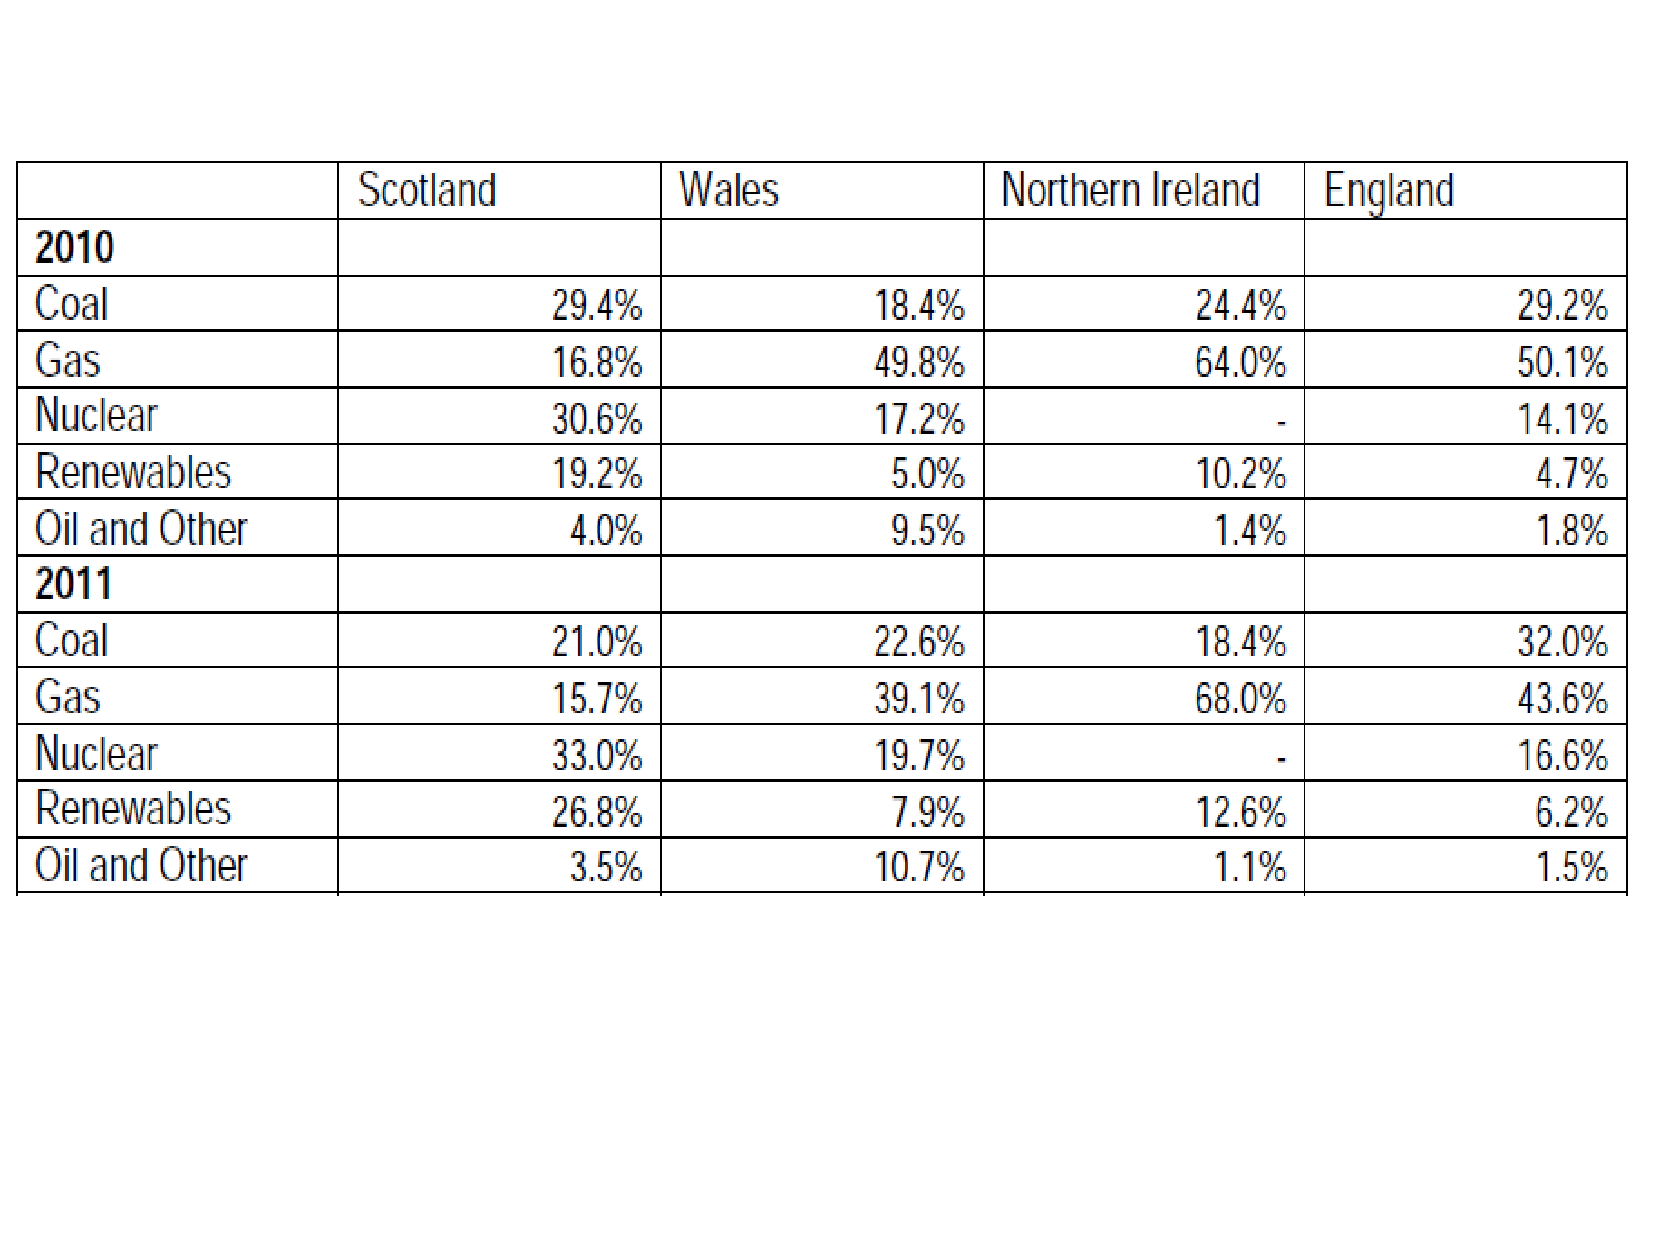
\includegraphics[width=9.cm,clip]{./Pics/Energy_Share_UK}
     \end{center}
    \end{figure}
\vspace{-2cm}
%\scriptsize
\textcolor{blue}{Fuel used in electricity generation and electricity supplied. (\href{https://www.gov.uk/government/organisations/department-of-energy-climate-change/series/electricity-statistics}{https://www.gov.uk/government/organisations/department-of-energy-climate-change/series/electricity-statistics})}
 \normalsize
\end{frame}


%%%
%%% Slide
%%%
\begin{frame}
 \frametitle{Introduction to Vapour and Gas Power}

    \begin{center}
     \begin{table}
       \begin{tabular}{l c c c}
    \hline
    \textcolor{blue}{Power Plant} & \textcolor{blue}{Renewable}  & \textcolor{blue}{Thermodynamic} \\
    \textcolor{blue}{Type}        & \textcolor{blue}{Source}     & \textcolor{blue}{Cycle}         \\
    \hline
      Coal                        &   No                         & Rankine  \\
      Natural Gas                 &   No                         & Brayton  \\
      Nuclear                     &   No                         & Rankine  \\
      Oil                         &   No                         & Rankine  \\
      Biomass                     &   Yes                        & Rankine  \\
      \textcolor{red}{Geothermal} &   Yes                        & \textcolor{red}{Rankine}  \\
      Solar                       &   Yes                        & Rankine  \\
      Hydroelectric               &   Yes                        & None     \\
      Wind                        &   Yes                        & None     \\
      Currents, tides and         &   Yes                        & None     \\
      waves                       &                              &          \\
    %\hline
    %\hline
      \end{tabular}
     \end{table}
    \end{center}
\end{frame}

%%%
%%% Slide
%%%
\begin{frame}
 \frametitle{Introduction to Vapour and Gas Power}
 %\scriptsize

    \begin{itemize}%\scriptsize
     \item <1-> While coal, natural gas, and nuclear still play important roles as energy sources, contributions from wind power, solar power, and other renewable sources are expected to be increasingly significant up to 2050;
     \item <2-> This table shows that thermodynamic cycles are crucial for a number of power plant types that employ renewable and non-renewable sources;
     \item <3-> The basic building block of vapour power systems is the \textcolor{blue}{Rankine cycle};
    % \item <4-> In fossil-fueled plants, the energy required for vaporisation originates in combustion of the fuel (i.e., coal, gas and oil) or fission of nuclear material;  
    \end{itemize}
 \normalsize
\end{frame}

%%%
%%% Slide
%%%
\begin{frame}
 \frametitle{Introduction to Vapour and Gas Power}
 %\scriptsize
Energy sources based on thermal-cycles (YouTube videos):
    \begin{itemize}%\scriptsize
     \item \href{http://www.youtube.com/watch?v=_UwexvaCMWA}{\textcolor{blue}{Nuclear Power Plants (NPP)}};
     \item \href{http://www.youtube.com/watch?v=0mjT8ETB128}{\textcolor{blue}{Coal-Fired Stations}};
     \item \href{http://www.youtube.com/watch?v=oi1TRbiE_Kw}{\textcolor{blue}{Gas Turbine Combined Cycle Power Plant}};
     \item \href{https://www.youtube.com/watch?v=kjpp2MQffnw}{\textcolor{blue}{Geothermal Power Plant}}.
    \end{itemize}
 \normalsize
\end{frame}

%%%
%%% Slide
%%%
\begin{frame}
 \frametitle{A Few Definitions}
 %%\scriptsize
 \begin{itemize}
  \item <1-> A \textcolor{blue}{cycle} is defined as a repeated series of operations occurring in a certain order. A system is said to have undergone a cycle if it returns to its initial state at the end of the process.  Cycles can be classified as ideal (where there is no heat losses) and real. 
  \item <2-> In \textcolor{blue}{gas cycles}, the working fluid remains in the gas phase throughout the cycle (e.g., air).
  \item <3-> In \textcolor{blue}{vapour cycles}, the working fluid exists as a vapour for part of the cycle and a liquid for the other part -- i.e., the working fluid is alternately vaporised and condensed.
  \item <4-> Steam is the most common working fluid in vapour power cycles as it has many desirable characteristics: low cost, availability and high enthalpy of vaporisation.
 % \item <5-> Coal, nuclear and natural gas power plants are examples of steam power plants. Each utilises a different type of fuel to supply heat to the steam cycle. 
  \item <5-> In \textcolor{blue}{closed cycles}, after each pass through the cycle the working fluid remains within the system.
  \item <6-> In \textcolor{blue}{open cycles}, after a few (or a single) pass through the cycle the working fluid is replaced by a fresh working fluid.
 \end{itemize}
 %\normalsize
\end{frame}


%%%
%%% SUB-SECTION
%%%
\subsection{Carnot Engines and Carnot Cycle}


%%%
%%% Slide
%%%
\begin{frame}
 %\scriptsize
 \frametitle{The Carnot Cycle}
  \begin{columns}
   \begin{column}[c]{0.6\linewidth}
    \begin{enumerate}[(a)] \scriptsize
     \item <1-> A \blue{heat engine} is a closed system that converts heat to work and operates in a cycle;
     \item <2-> A \blue{Carnot cycle} has four reversible steps, alternating isothermal (and \blue{isobaric:} 4-1, 2-3) and frictionless adiabatic (i.e., \blue{isentropic:} 1-2, 3-4):
       \begin{enumerate}[(i)]\scriptsize
         \item <3-> {\it Step 1-2}: \blue{Steam} is \red{isentropically} expanded to $T_{2}$ and $P_{2}$;
         \item <4-> {\it Step 2-3}: Heat is rejected at \red{constant pressure} $\left(P_{2}\right)$ \red{and temperature} $\left(T_{2}\right)$. During this step, steam becomes wetter and cooled;
         \item <5-> {\it Step 3-4}: Wet steam is \red{isentropically} compressed until the steam returns to its original state at $T_{1}$ and $P_{1}$ (saturated liquid);
         \item <6-> {\it Step 4-1}: \blue{Boiling water} at temperature $T_{1}$ is heated to form wet steam $\left(\right.$dryness fraction $x_{1}\left.\right)$. Heat is then absorbed at \red{constant temperature} $\left(T_{1}\right)$ \red{and pressure} $\left(P_{1}\right)$;
       \end{enumerate}
     \item <7-> The efficiency of the \blue{Carnot cycle} is given by:
          \visible<7->{\begin{equation}
             \blue{\eta_{\text{Carnot}}} = \frc{\text{Work Done}}{\text{Heat Supplied}} \blue{= 1 - \frc{T_{2}}{T_{1}}}
          \end{equation}}
    \end{enumerate} 
   \end{column}
   \begin{column}[c]{0.4\linewidth}
   \begin{figure}%
    \begin{center}
     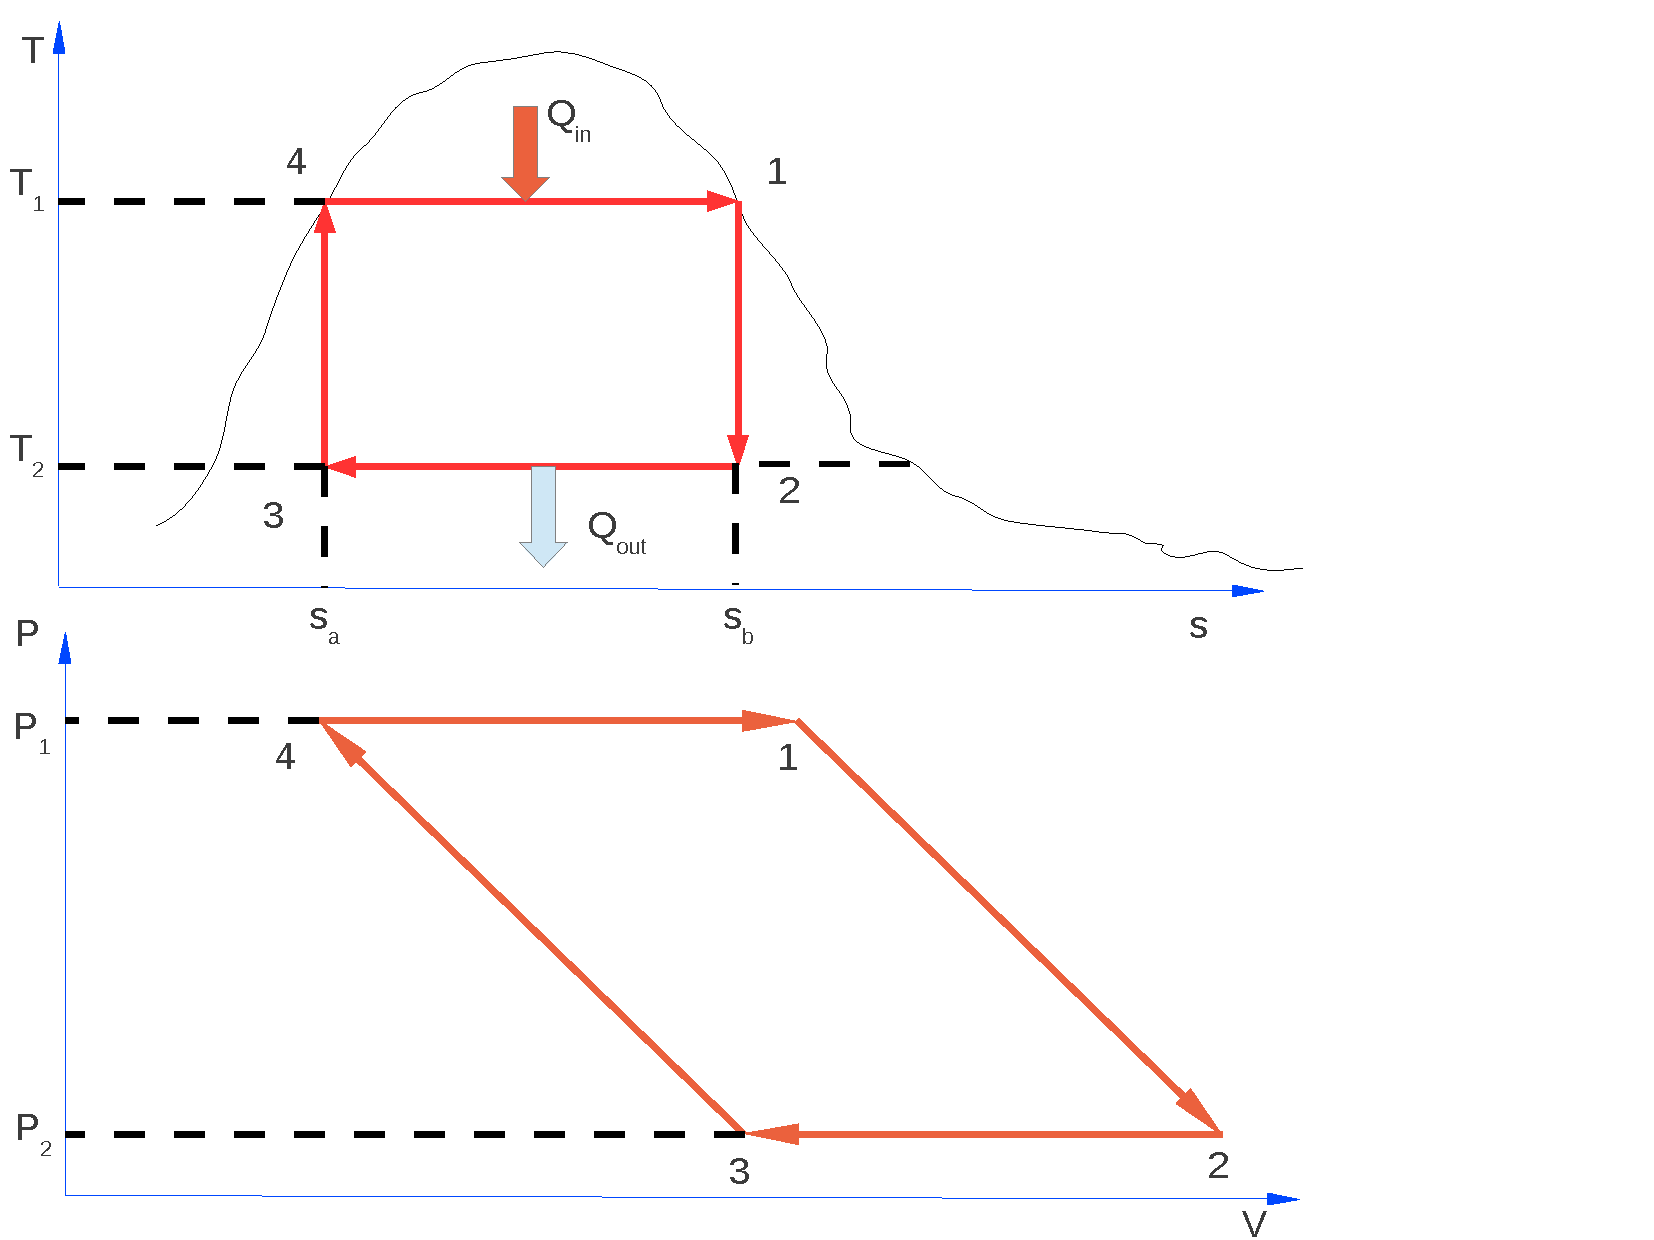
\includegraphics[width=5.5cm,clip]{./Pics/Carnot_PV_TS}
    \end{center}
   \end{figure}    
   \end{column}
  \end{columns}
 \normalsize
\end{frame}

%%%
%%% Slide
%%%
\begin{frame}
 \frametitle{Limitations of the Carnot Cycle}
 %\scriptsize
 \begin{enumerate}[(a)]
  \item <1-> The \blue{Carnot cycle} is thermodynamically simple and has the \red{highest thermal efficiency} for a given temperature gradient;
  \item <2-> It is however {\it difficult to operate in practice} due to:
  \begin{enumerate}[(i)] %\scriptsize
   \item <3-> It is difficult to \underline{compress a wet vapour isentropically} to the saturated state (as required by the process 3-4);
   \item <4-> It is difficult to \underline{control the quality of the condensate} produced by the condenser to reach state 3;
   \item <5-> The \blue{efficiency is greatly affected by $T_{1}$} at which heat is transferred to the working fluid. As the critical temperature of steam is 374$^{\circ}$C therefore, if the cycle is to be operated in the wet region, the maximum possible temperature is severely limited;
   \item <6-> The cycle is even more difficult to operate in practice with superheated steam due to the necessity to \blue{supply superheated steam at constant temperature instead of constant pressure} (as it is usual in industrial plants);
   \item <7-> \red{\it In a practical cycle, limits of pressure and volume are easier to be obtained than limits of temperature}; 
   \item <8-> Therefore \blue{\underline{no} practical engine operates in the Carnot cycle}, although all modern cycles aspire to achieve it.
  \end{enumerate}
 \end{enumerate}
 \normalsize
\end{frame}


%%%
%%% SUBSECTION
%%%
\subsection{The Rankine Cycle}


%%%
%%% Slide
%%%
\begin{frame}
 \frametitle{Rankine Cycle}
 %\scriptsize
 \begin{columns}
   \begin{column}[c]{0.5\linewidth}
    \begin{figure}%
     \begin{center}
      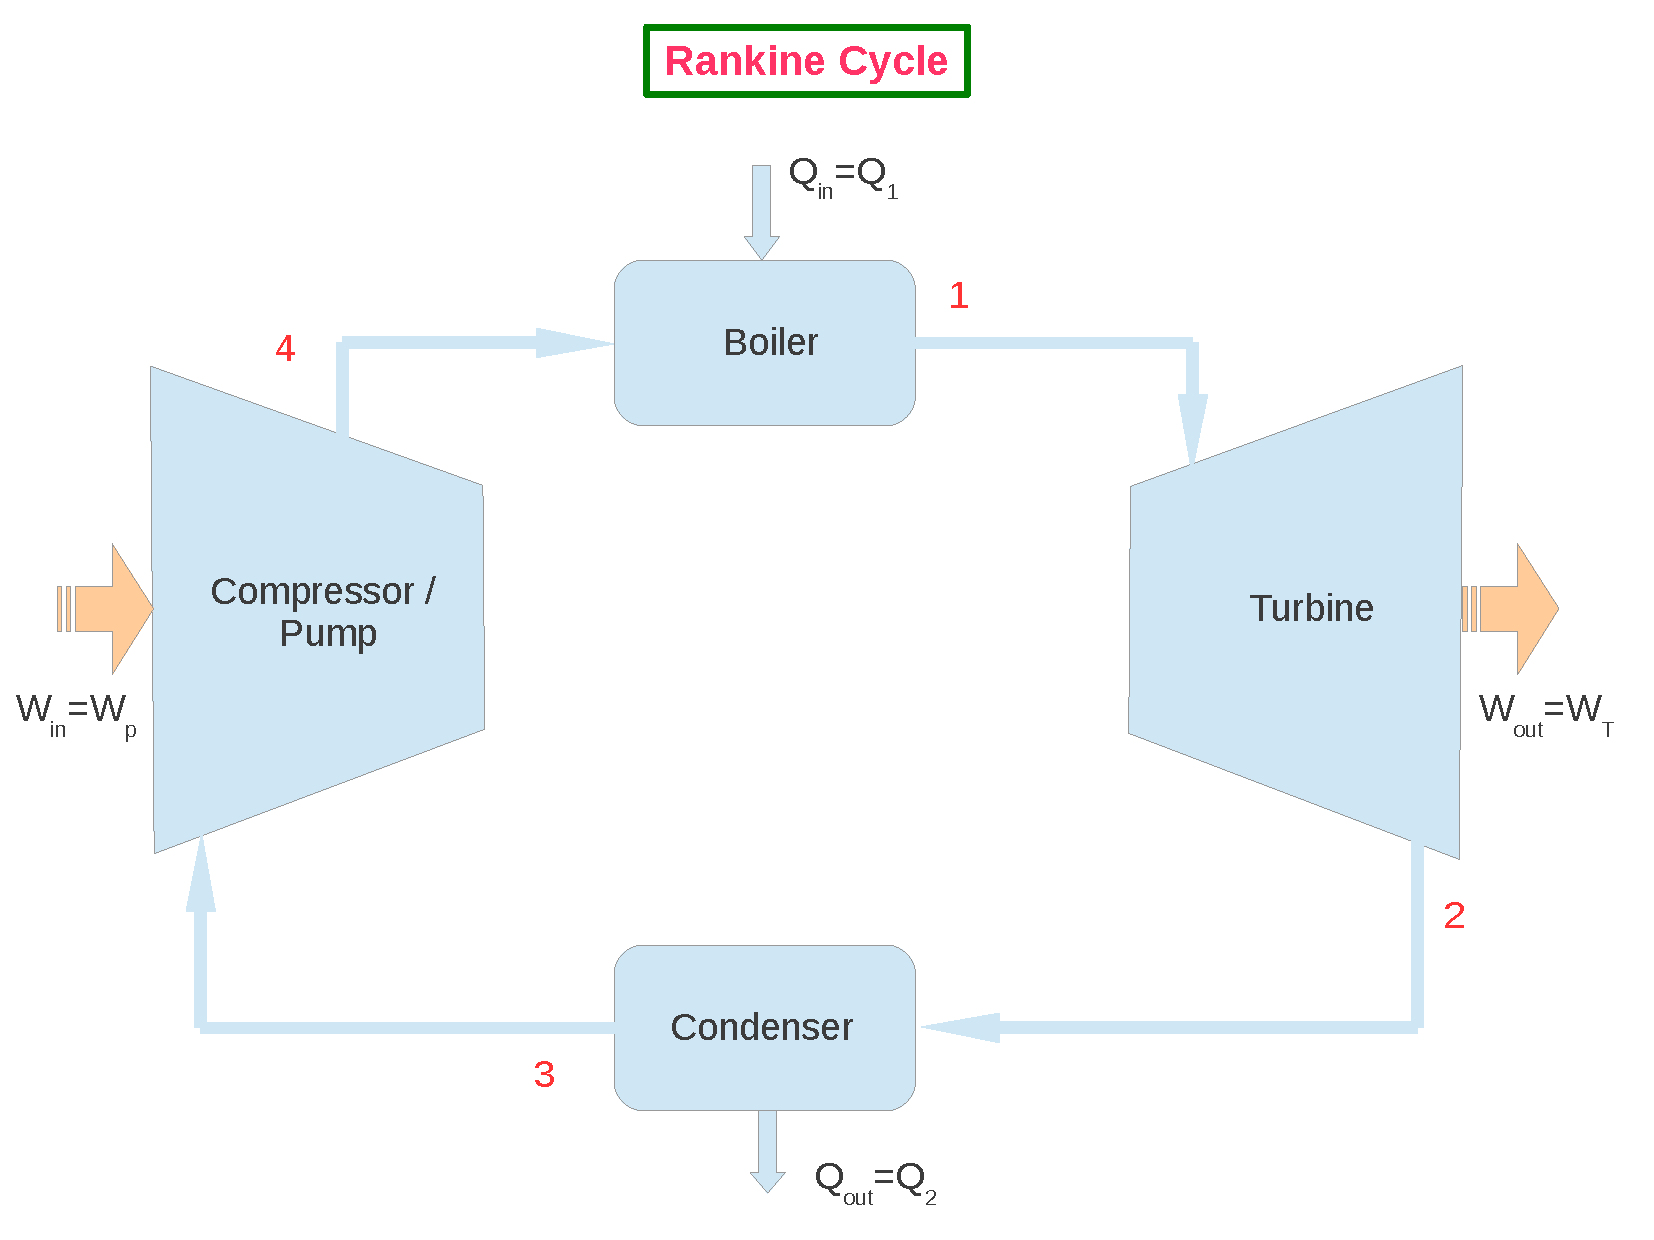
\includegraphics[width=6.5cm,clip]{./Pics/Simple_Rankine_Cycle}
     \end{center}
    \end{figure}  
   \end{column}
   \begin{column}[l]{0.5\linewidth}
    \begin{enumerate}[(a)]\scriptsize
     \item<1->\textcolor{blue}{Rankine Cycle} (RC) is the ideal cycle for vapour power plants;
     \item<2-> It does not involve any internal irreversibilities and consists of the following four processes:
     \begin{enumerate}[(i)]\scriptsize
      \item<3-> \textcolor{red}{Process 1-2}: reversible adiabatic (i.e., \blue{isentropic}) expansion in the turbine (or steam engine);
      \item<4-> \textcolor{red}{Process 2-3}: constant-pressure heat transfer in the condenser;
      \item<5-> \textcolor{red}{Process 3-4}: reversible adiabatic (i.e., \blue{isentropic}) pumping process in the feed pump;
      \item<6-> \textcolor{red}{Process 4-1}: constant-pressure heat transfer in the boiler.  
     \end{enumerate}
     \item<7-> Efficiency of the \blue{RC} can be expressed as:
       \visible<7->{\begin{eqnarray}
          \blue{\eta_{\text{Rankine}}} &=& \frc{W_{\text{net}}}{Q_{1}} = \frc{W_{T}-W_{P}}{Q_{1}}\nonumber \\
                                    &=& \frc{\left(h_{1}-h_{2}\right)-\left(h_{f4}-h_{f3}\right)}{h_{1}-h_{f4}} \nonumber \\
                                    &=& \blue{\frc{h_{1}-h_{2}}{h_{1}-h_{f4}}} 
       \end{eqnarray}}
    \end{enumerate}
   \end{column}
  \end{columns}
 \normalsize
\end{frame}


%%%
%%% Slide
%%%
\begin{frame}
 \frametitle{Rankine Cycle: {\it Pv}, {\it Ts} and {\it hs} Diagrams}
 %\scriptsize
 \begin{columns}
%
   \begin{column}[l]{0.45\linewidth}
    \begin{figure}%
     \begin{center}
      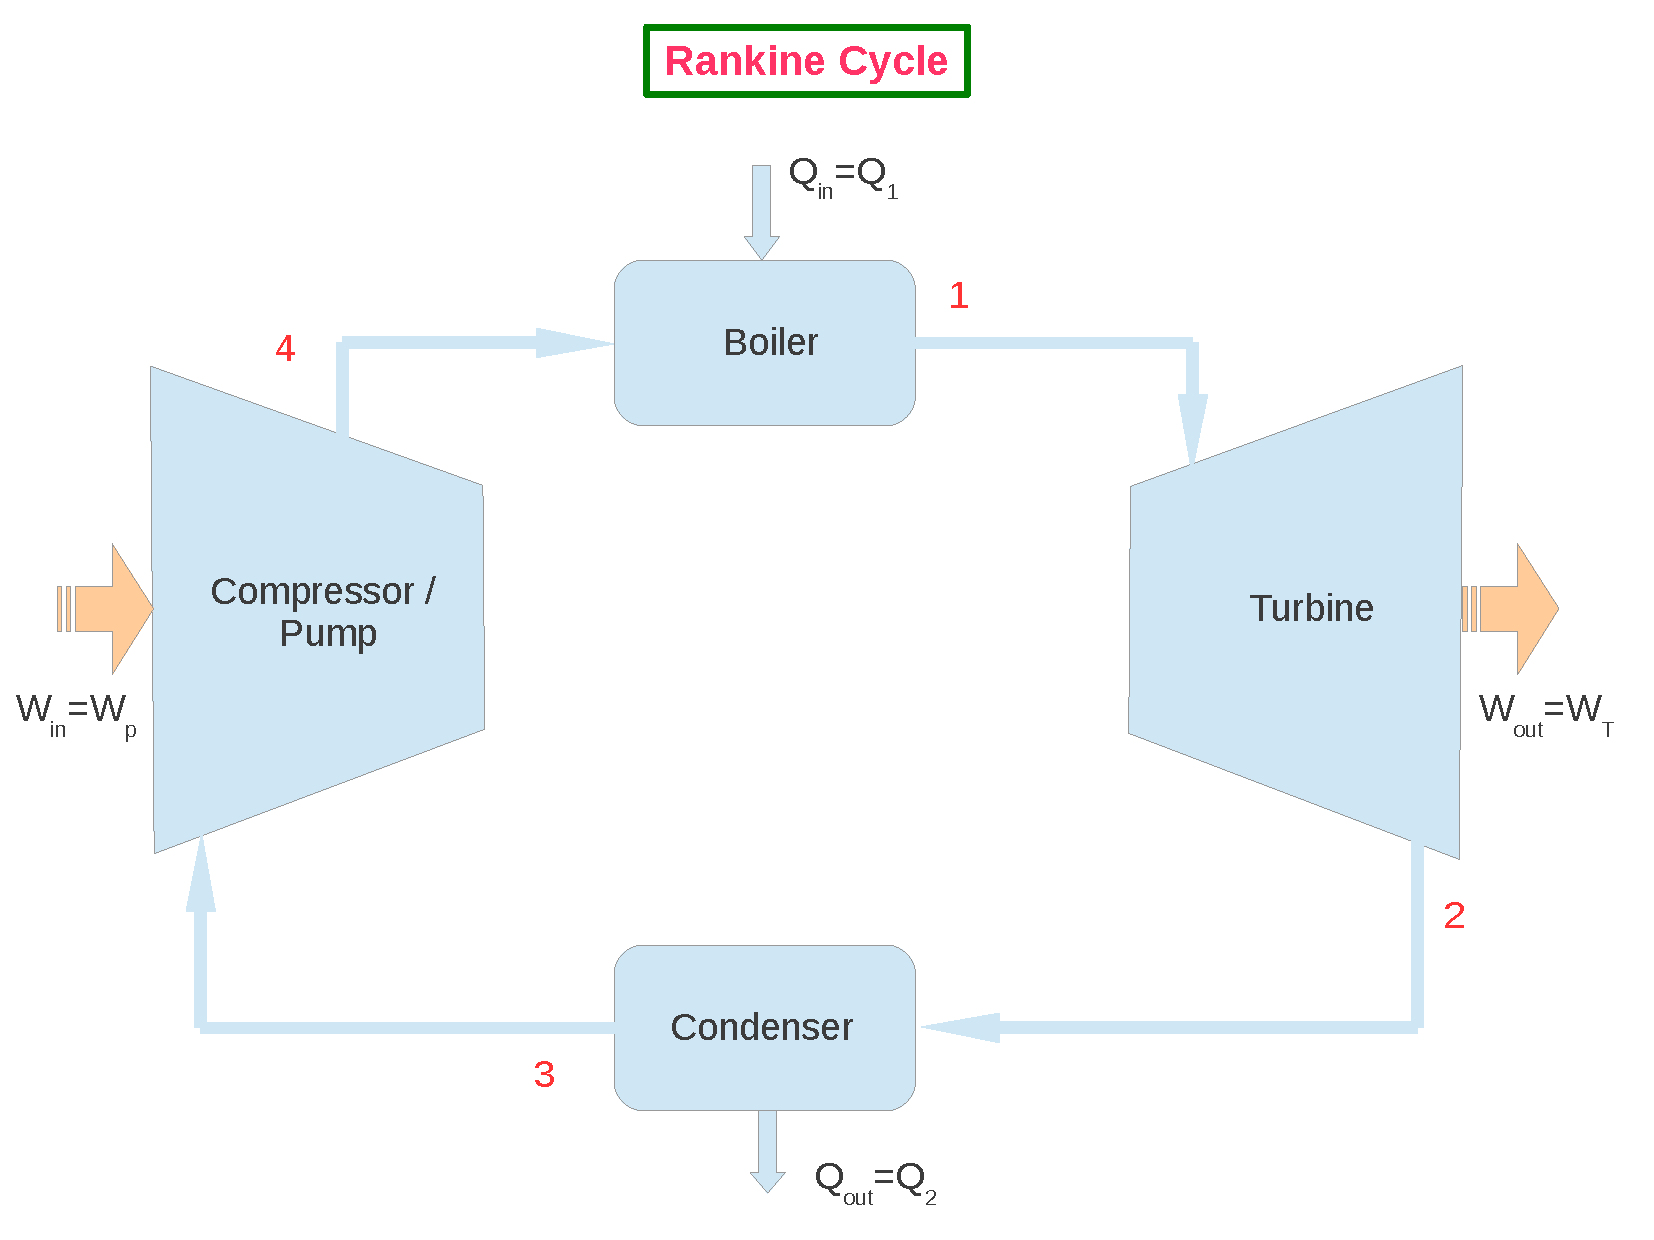
\includegraphics[width=5.5cm,clip]{./Pics/Simple_Rankine_Cycle}
     \end{center}
    \end{figure} 
    \begin{block}{\begin{center}Quality of the Vapour\end{center}}
       \begin{equation}\scriptsize
         \blue{x_{j} = \frc{\Psi_{j}-\Psi_{f}}{\Psi_{g}-\Psi_{f}}} \;\;\;\text{with }\Psi=\left\{h,s\right\}
       \end{equation}
    \end{block}
   \end{column}
%
   \begin{column}[c]{0.55\linewidth}
    \begin{figure}%
     \begin{center}
      \visible<2->{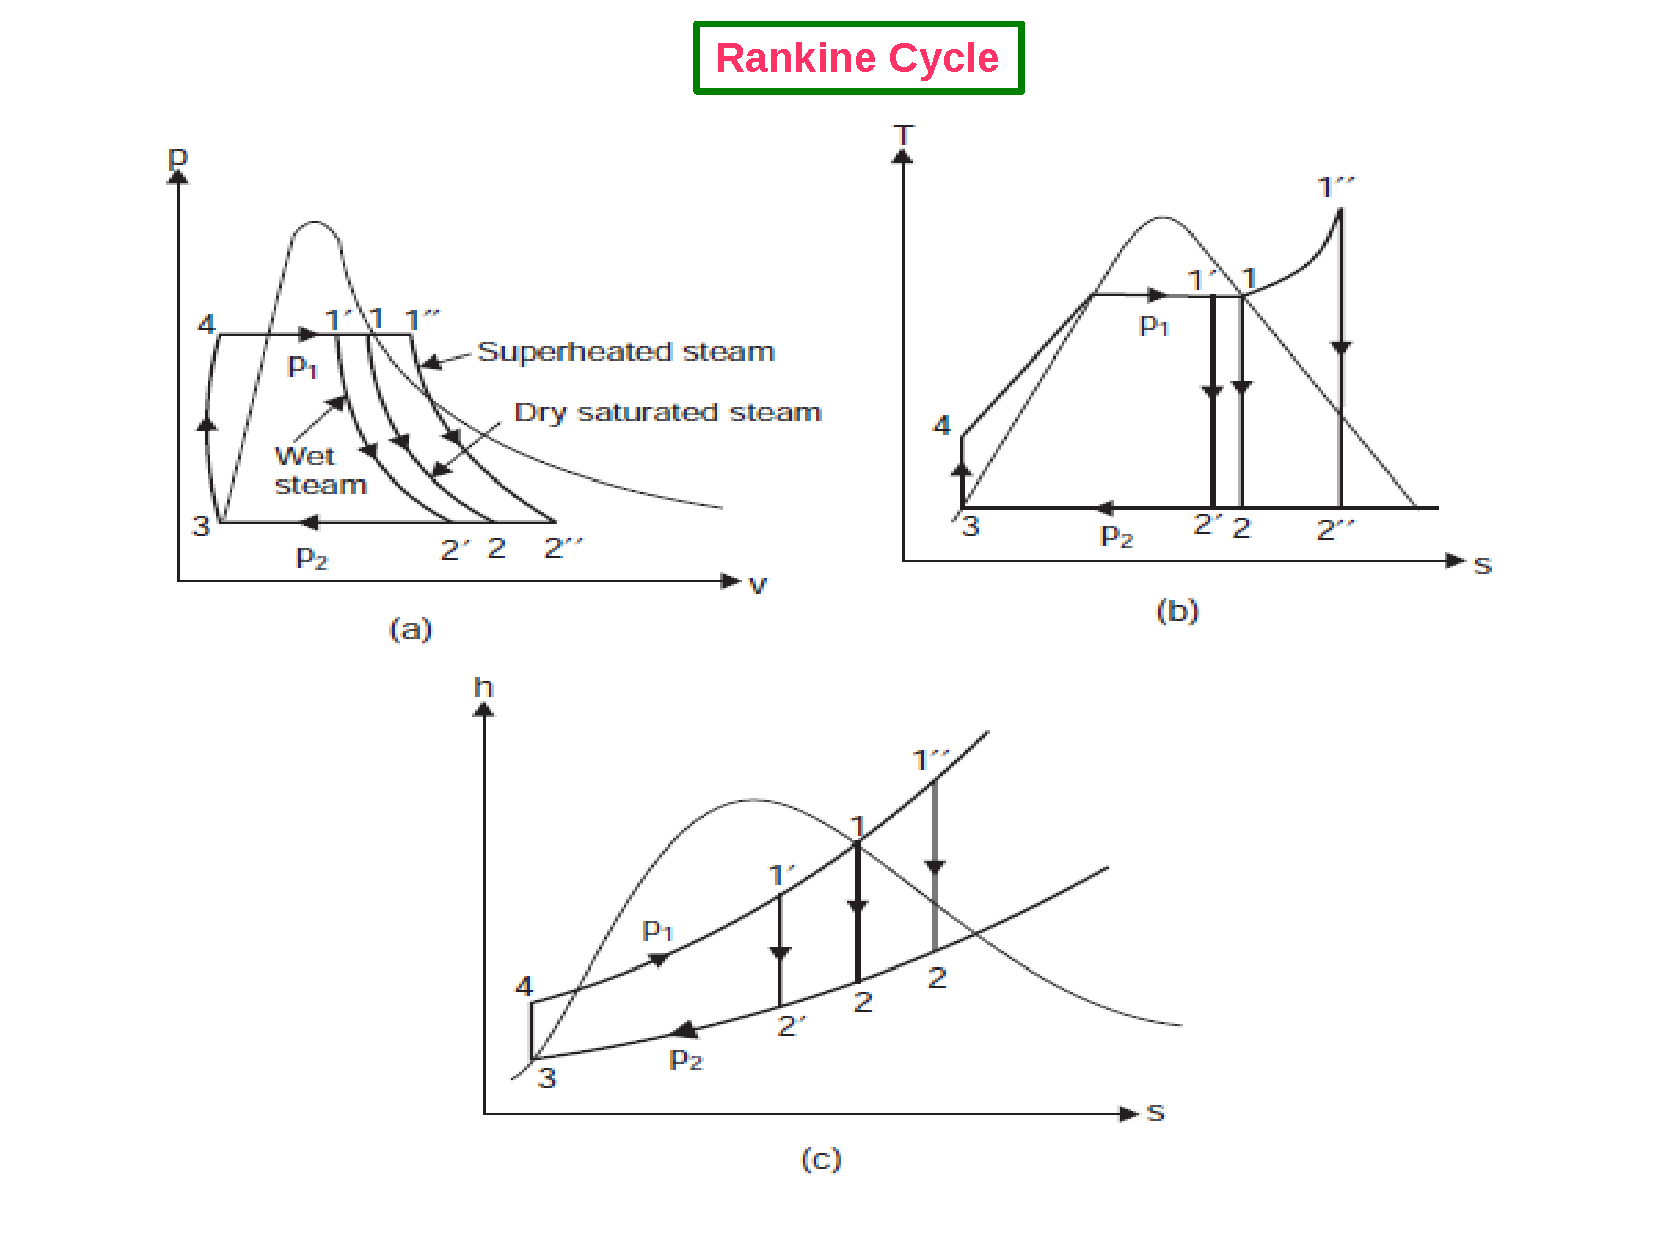
\includegraphics[width=7.5cm,clip]{./Pics/Simple_Rankine_Cycle_Diagrams}}
     \end{center}
    \end{figure}  
   \end{column}
  \end{columns}
\end{frame}


%%%
%%% Slide
%%%
\begin{frame}
 \frametitle{Ideal {\it versus} Actual Rankine Cycles}
   \begin{columns}
      \begin{column}[c]{0.5\linewidth}
         \begin{enumerate}\scriptsize
             \item<1-> Differences between actual and ideal RC are mainly due to \blue{fluid friction} resulting in \blue{pressure drop in the boiler, condenser and pipes};
             \item<2-> Steam leaves the boiler at a pressure lower than expected; 
             \item<3-> \underline{Fluid pressure at the turbine inlet} is also \underline{lower than that at the boiler exit} due to pressure drop between pipes; 
             \item<4-> Pressure drop in the \blue{condenser} is usually \underline{negligible}; 
             \item<5-> In order to mitigate these pressure drops throughout power cycles, water must be pumped to a pressure higher than the required in the ideal cycle. Thus, a more powerful pump (and therefore larger worker input to the pump) is needed, increasing the energy cost.  
         \end{enumerate}\scriptsize
         \visible<6->{\begin{block}{\begin{center}Efficiencies of Turbines and Pumps\end{center}}
           \begin{eqnarray}\scriptsize
              && \blue{\eta_{T}=} \frc{W_{T,a}}{W_{T,s}} = \blue{\frc{h_{2}-h_{1}}{h_{2s}-h_{1}}} \\
              && \blue{\eta_{P}=} \frc{W_{P,s}}{W_{P,a}} = \blue{\frc{h_{4s}-h_{3}}{h_{4}-h_{3}}}
           \end{eqnarray}
         \end{block}}
      \end{column}
      \begin{column}[c]{0.5\linewidth}
         \vbox{
           \hbox{\hspace{.5cm}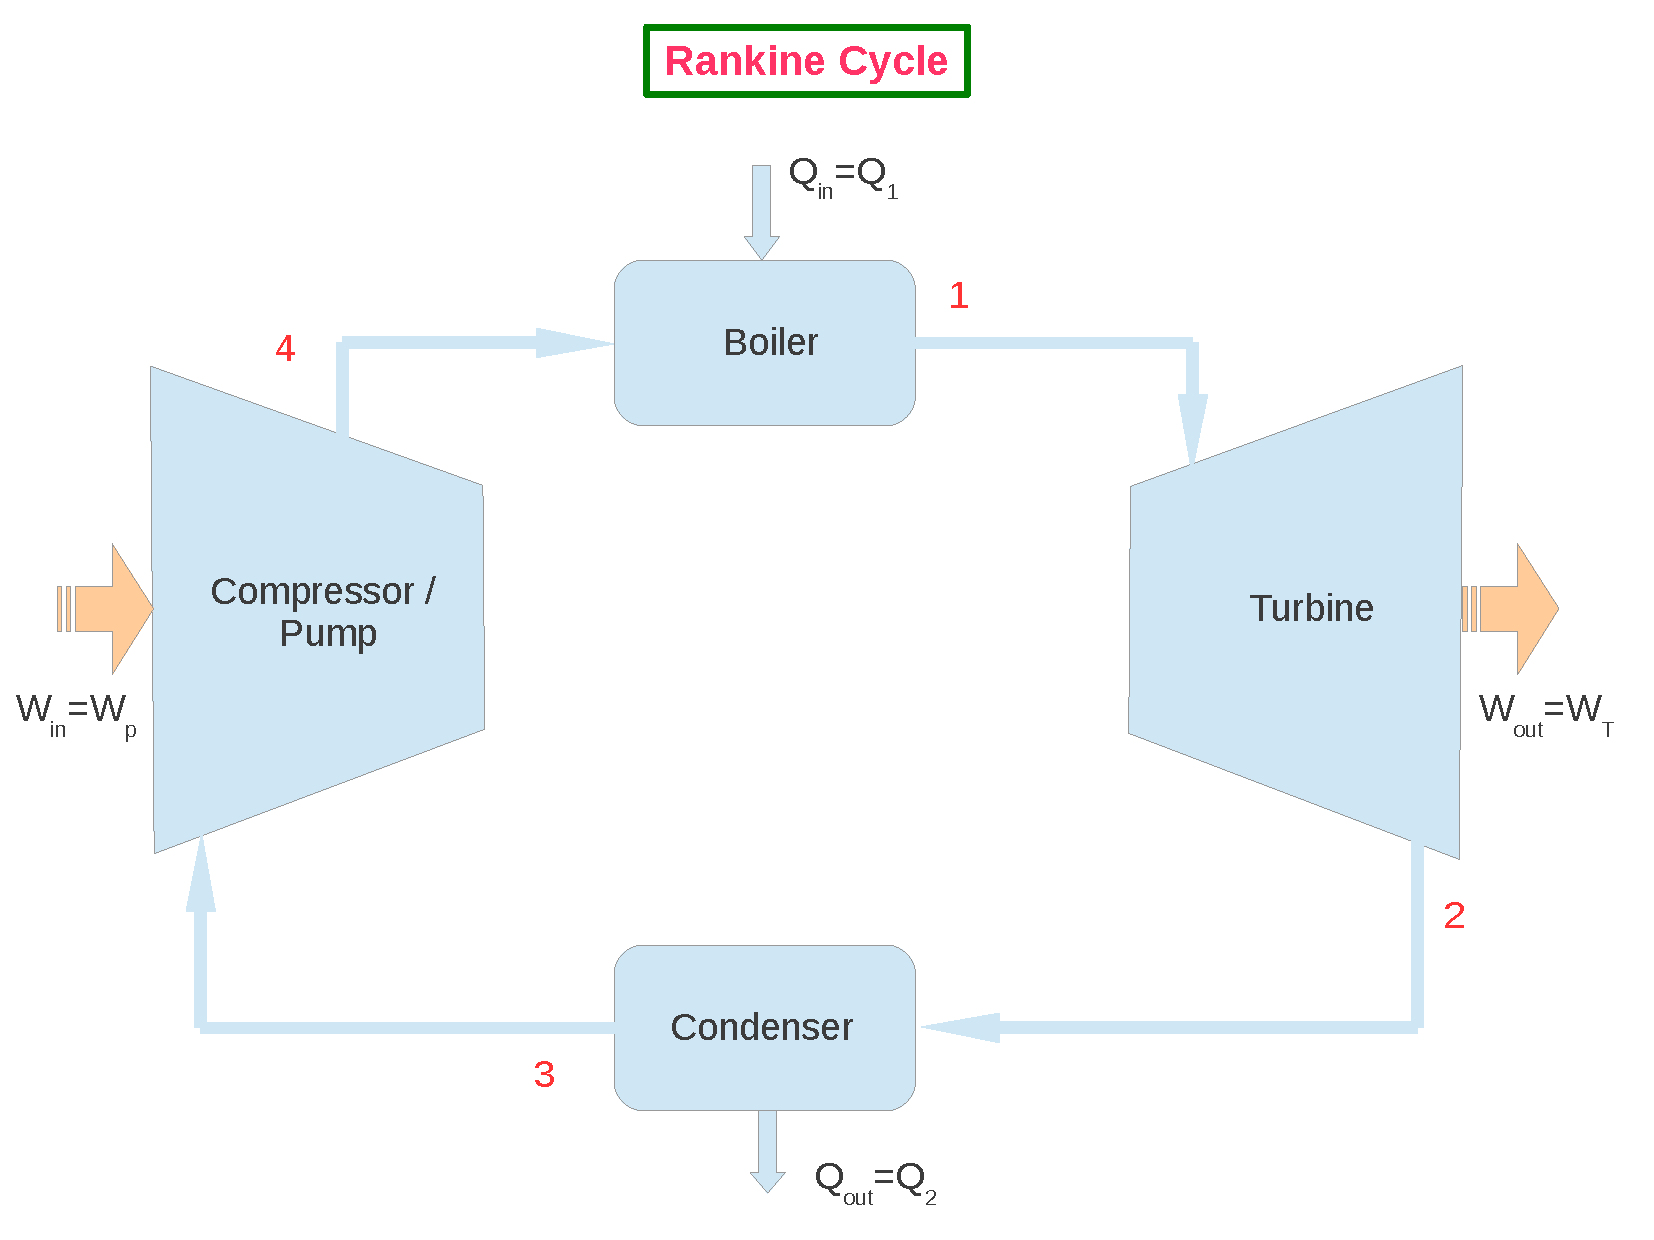
\includegraphics[width=5.cm,clip]{./Pics/Simple_Rankine_Cycle}}
           \vspace{-0.1cm}
           \hbox{\hspace{.5cm}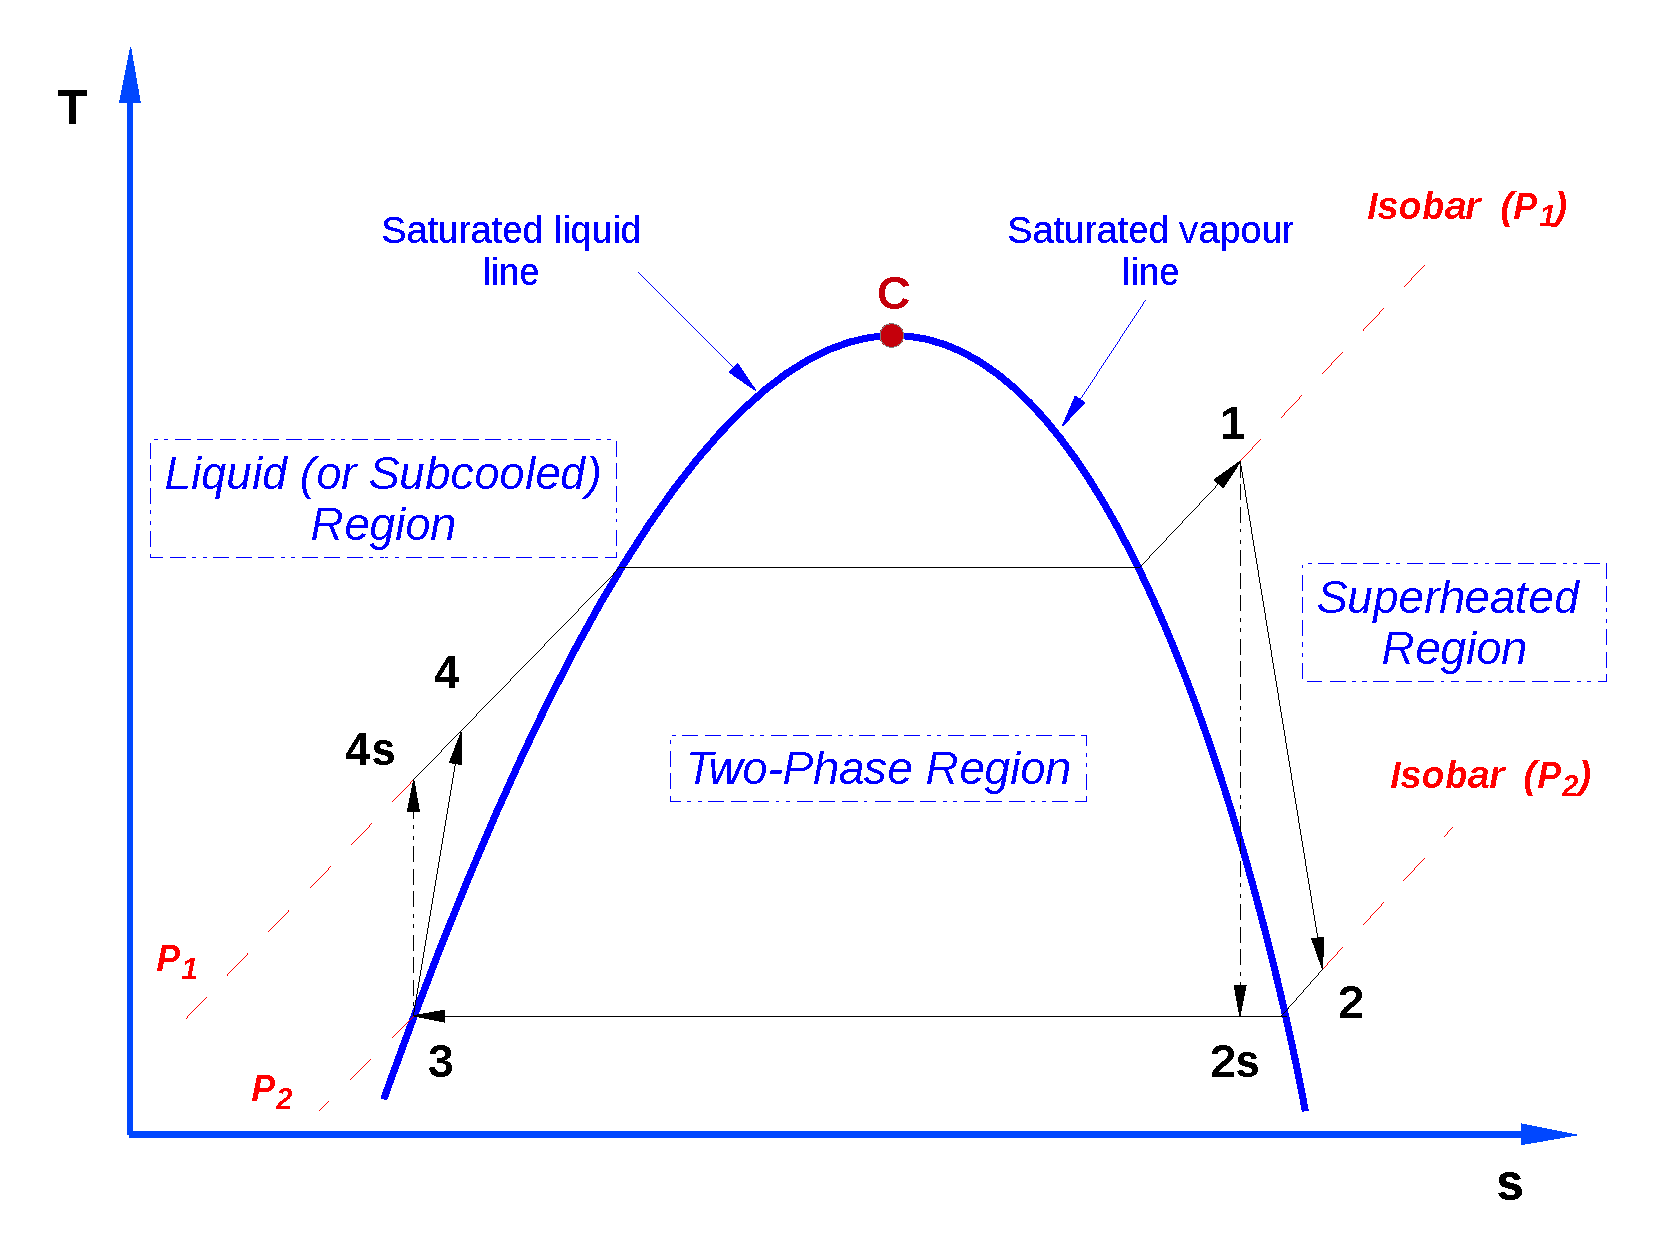
\includegraphics[width=5.5cm,clip]{./Pics/Ideal_Real_Rankine}}
         }
      \end{column}
   \end{columns}
 \normalsize
\end{frame}

%%%
%%% Slide
%%%
\begin{frame}
 \frametitle{Improving the Efficiency of the Rankine Cycles}
   \begin{columns}
      \begin{column}[c]{0.5\linewidth}
         \begin{enumerate}\scriptsize
            \item<1-> The efficiency of the Rankine cycle may be improved by:
              \begin{enumerate}[(a)]\scriptsize
                 \item <1-> Increasing the average temperature at which heat is transferred to the working fluid in the boiler or;
                 \item <1-> Reducing the temperature at which the heat is transferred from the working fluid in the condenser;
              \end{enumerate} 
            \item <2-> This can be achieved with:
              \begin{enumerate}[(a)]\scriptsize
                 \item <2-> Increasing boiler pressure;
                 \item <2-> Use of superheated steam;
                 \item <2-> Reducing condenser pressure.
              \end{enumerate}
            \item <3-> The thermal efficiency can be improved by
              \begin{enumerate}[(a)]\scriptsize
                 \item <3-> Regenerative feed heating;
                 \item <3-> Reheating of steam;
                 \item <3-> Water extraction;
                 \item <3-> Using binary-vapour
              \end{enumerate}
         \end{enumerate}  
      \end{column}
      \begin{column}[c]{0.5\linewidth}
         \visible<2->{\begin{figure}%
           \begin{center}
              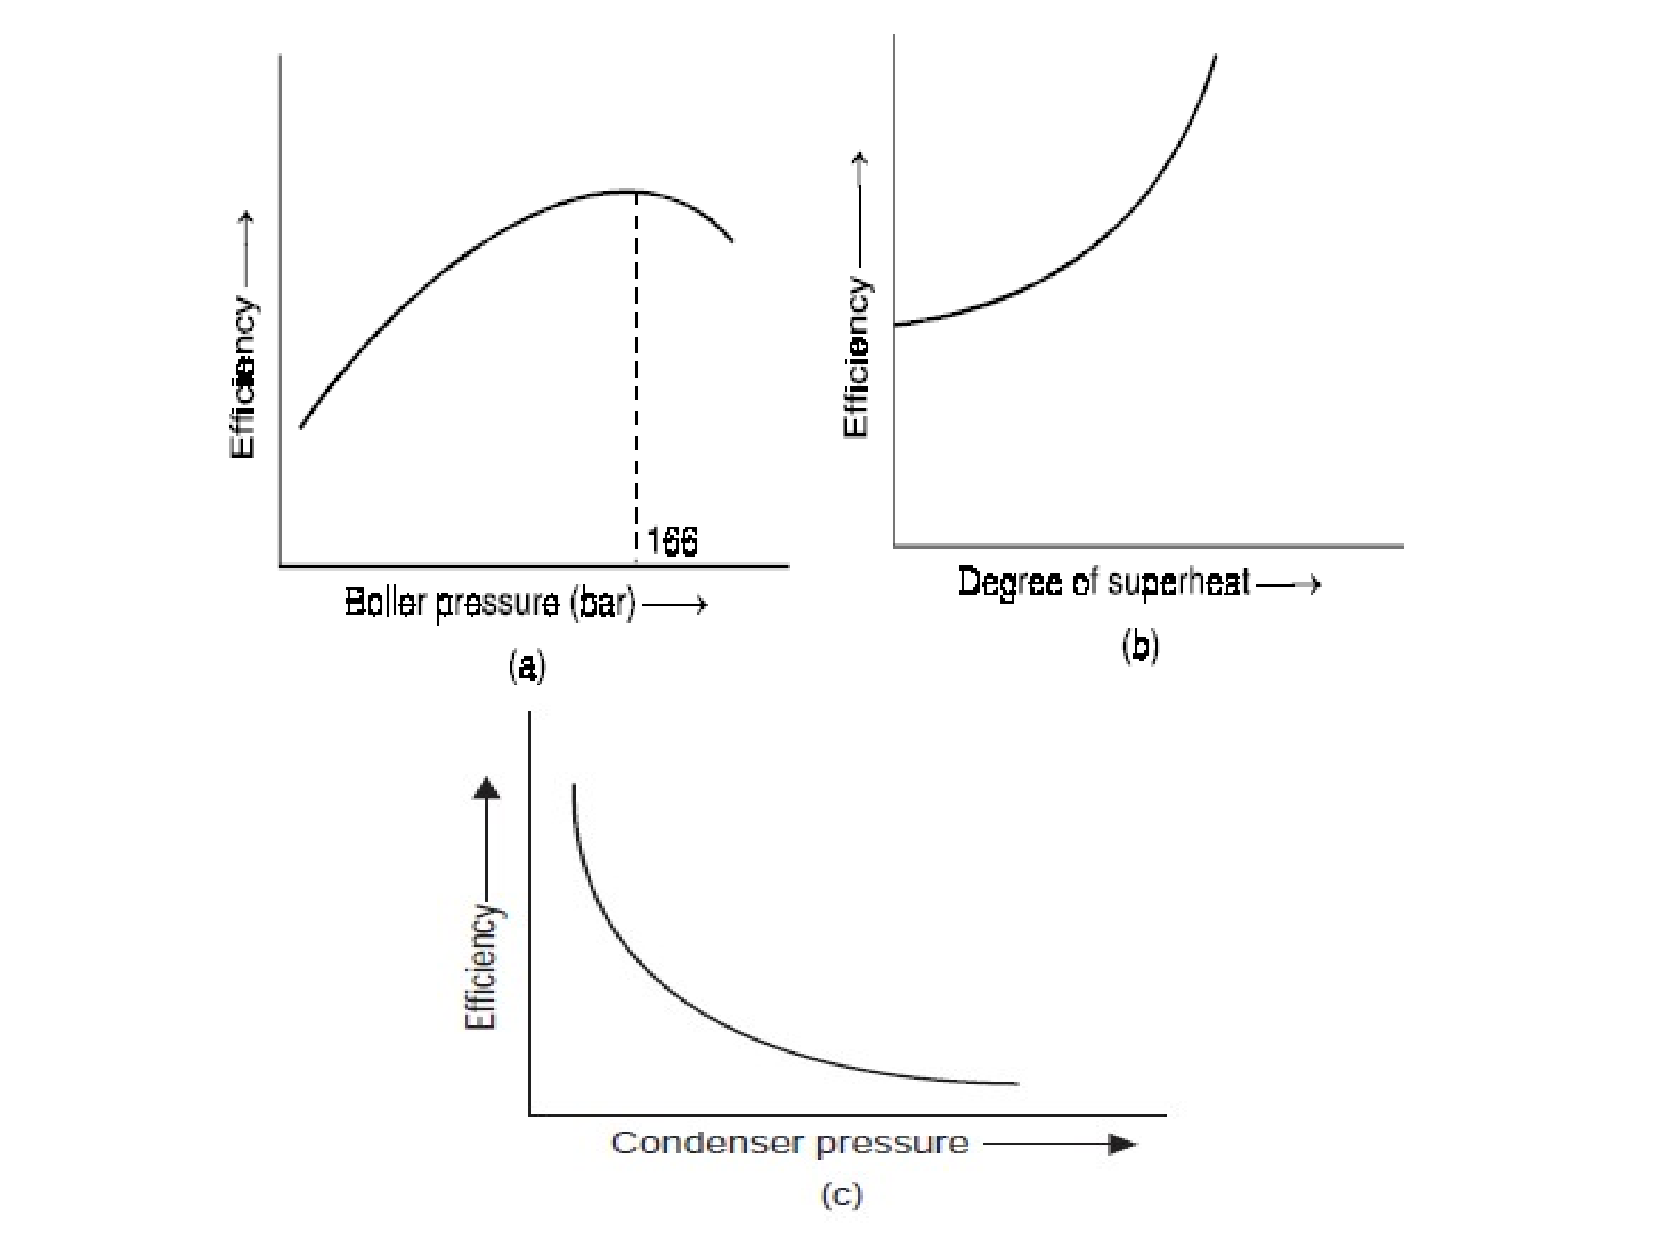
\includegraphics[width=7.cm,clip]{./Pics/Rankine_Improving_Efficiency}
           \end{center}
         \end{figure}}
      \end{column}
   \end{columns}
 \normalsize
\end{frame}

%%%
%%% SUBSECTION
%%%
\subsection{Examples}

%%%
%%% Slide
%%%
\begin{frame}
 \frametitle{Example 1: Carnot and Rankine efficiencies (Problem 1)}
 %\scriptsize
    Steam (dry and saturated) is supplied by the boiler at 15 bar and the condenser pressure is 0.4 bar. Calculate the Carnot and Rankine efficiencies of the cycle. Neglect the pump work.
\end{frame}

%%%
%%% Slide
%%%
\begin{frame}
 \frametitle{Example 2: Ideal Rankine Cycle (Problem 5)}
 %\scriptsize
Water is the working fluid in an ideal Rankine cycle. Dry saturated vapour enters the turbine at 16 MPa, and the condenser pressure is 8 kPa. The mass flow rate of steam entering in the turbine is 120 kg/s. Calculate:
\begin{enumerate}[(a)]
\item the net power developed (in MW);
\item rate of heat transfer to the steam passing through the boiler (in MW);
\item thermal efficiency;
\item mass flow rate of the condenser cooling water (in kg/s), if the cooling water undergoes a temperature increase of 18$^{\circ}$C with negligible pressure change in passing through the condenser. Assume that the heat capacity at constant pressure $\left(\text{C}_{\text{p}}\right)$ of the cooling water is 4.18 $\frac{\text{kJ}}{\text{kg.}^{\circ}\text{C}}$.
\end{enumerate} 
\end{frame}

%%%
%%% Slide
%%%
\begin{frame}
 \frametitle{Example 3: Simple Steam Power Plant (Problem 2)}
 \scriptsize
   The table below represents the steps of an idealised steam power plant:
    \begin{center}
     \begin{tabular}{||c | c | c | c | c | c ||}
      \hline\hline
       {\bf Step} & {\bf Location}       & {\bf Pressure}  & {\bf Temperature}     & {\bf Quality /}  &{\bf Velocity}    \\
                  &                      & {\bf (bar)}     &{\bf$\left(^{\circ}\text{C}\right)$}& {\bf State} & {\bf m/s} \\
      \hline\hline
          1       & Inlet to turbine     &   60            &   380                 &  --              &       --         \\
      \hline
          2       & Exit from turbine and&   0.1           &    --                 & 0.9              &  200             \\
                  & inlet to condenser   &                 &                       &                  &                  \\ 
      \hline
          3       & Exit from condenser and&  0.09         &  --                   & Saturated        &  --              \\
                  & inlet to pump        &                 &                       & Liquid           &   --             \\
      \hline
          4       & Exit from pump and   &  100            &   --                  &     --           &   --             \\
                  & inlet to boiler      &                 &                       &                  &                  \\
      \hline 
          5       & Exit from boiler     &  80             &  440                  &      --          &    --            \\
           \hline\hline
     \end{tabular}
    \end{center}
    Assume that the steam mass flow rate leaving the boiler is 10$^{4}$ kg.h$^{-1}$. Sketch the cycle numbering each stage. Calculate:
      \begin{enumerate}[(a)]
         \item Specific enthalpies of all streams;
         \item Power output of the turbine;
         \item Heat transfer per hour in the boiler and condenser;
         \item Mass rate of cooling water circulated (kg/h) in the condenser assuming inlet and outlet fluid temperatures from the condenser of 20$^{\circ}$C and 30$^{\circ}$C. Assume that the heat capacity at constant pressure $\left(\text{C}_{\text{p}}\right)$ of the cooling water is 4.18 $\frac{\text{kJ}}{\text{kg.}^{\circ}\text{C}}$.
         \item Diameter (m) of the pipe connecting the turbine with the condenser;
         \item Sketch the $Ts$ diagram, indicating each step of the cycle.
    \end{enumerate}
 \normalsize
\end{frame}


%%%
%%% SECTION
%%%
\section{Modified Rankine Cycles}

\subsection{Reheat Rankine Cycle}

%%%
%%% Slide
%%%
\begin{frame}
 \frametitle{Ideal Reheat Rankine Cycle}
  \begin{columns}
     \begin{column}[c]{0.5\linewidth}
        \begin{enumerate}[(a)] \scriptsize
           \item<1-> Thermal efficiency can be enhanced by increasing the boiler pressure;
           \item<1-> However, this results in higher moisture content in the steam flow which can damage the turbine;
           \item<2-> To overcome this problem we may:
           \begin{enumerate}[(i)] \scriptsize
             \item<2-> Superheat the steam before the turbine: this would improve thermal efficiency of the cycle but the very high temperature may be prohibitive as novel (and more expansive) materials would need to be used;
             \item<2-> \blue{Expand the steam in the turbine in two stages and reheat in between}. This is an improvement on the ideal Rankine cycle as we would add a reheating process between continuous expansion.
           \end{enumerate}
           \item<3-> The \underline{main objective of using superheated steam} is \blue{to avoid excessive moisture in the steam} at the end of the expansion process (maximum moisture content $\sim$ 12$\%$ to avoid turbine blades' damage);
           \item<4-> Advantages of Reheating:
              \begin{enumerate}[(i)]\scriptsize
                 \item<4-> Increase power output from the turbine;
                 \item<4-> Low erosion and corrosion issues;
                 \item<4-> Improvement of the thermal efficiency of the turbines.
              \end{enumerate}
        \end{enumerate}
     \end{column}
     \begin{column}[c]{0.5\linewidth} 
        \visible<2->{\begin{figure}%
           \begin{center}
             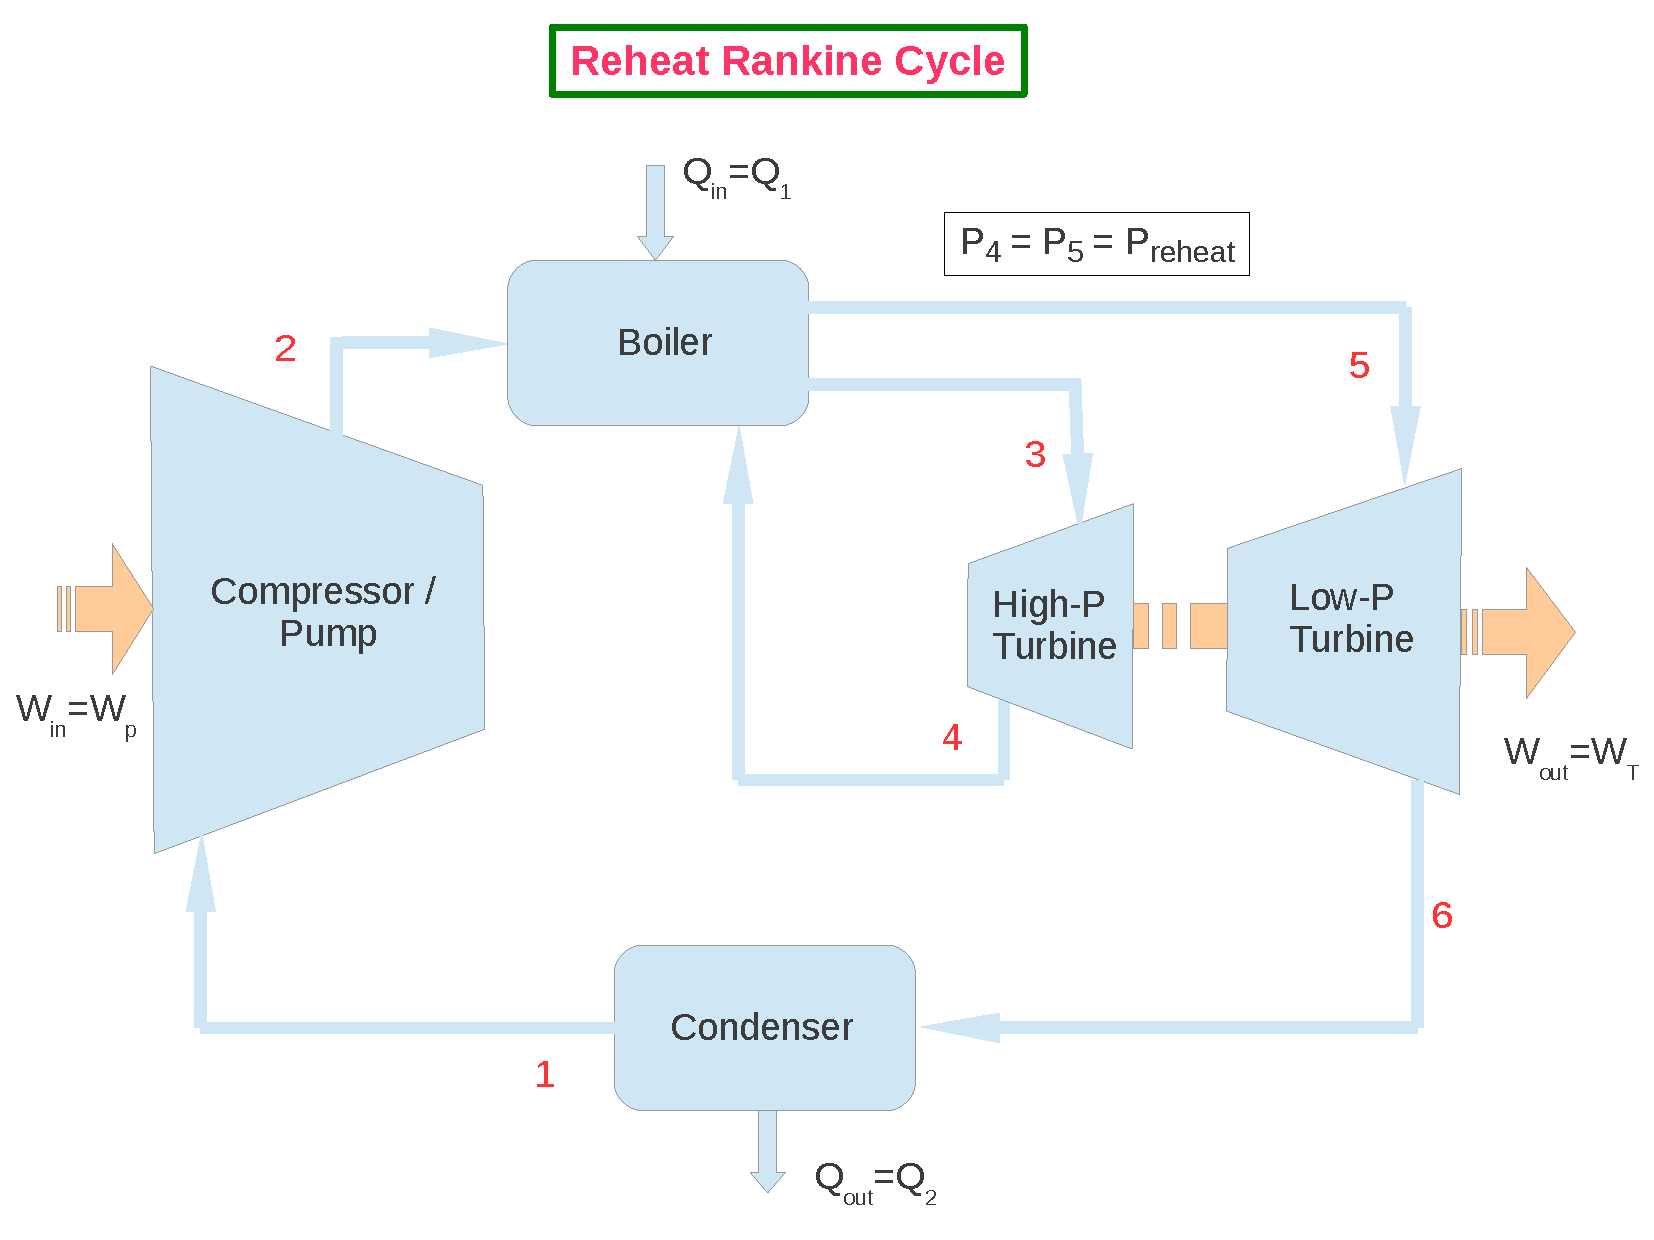
\includegraphics[width=6.25cm,clip]{./Pics/Reheat_Rankine_Cycle}
           \end{center}
        \end{figure}} 
        \begin{enumerate}[(a)]\scriptsize\setcounter{enumi}{5}
           \item<5-> Disadvantages of Reheating:
              \begin{enumerate}[(i)]\scriptsize
                 \item<5->Reheating requires more maintenance;
                 \item<5->Enhancement of thermal efficiency may not be enough to match the larger costs associated with reheating the steam.
              \end{enumerate}
        \end{enumerate}
     \end{column}
  \end{columns}
 \normalsize
\end{frame}


%%%
%%% Slide
%%%
\begin{frame}
 \frametitle{Ideal Reheat Rankine Cycle}
  \begin{columns}
     \begin{column}[c]{0.5\linewidth} 
       \begin{center}
          \begin{figure}
             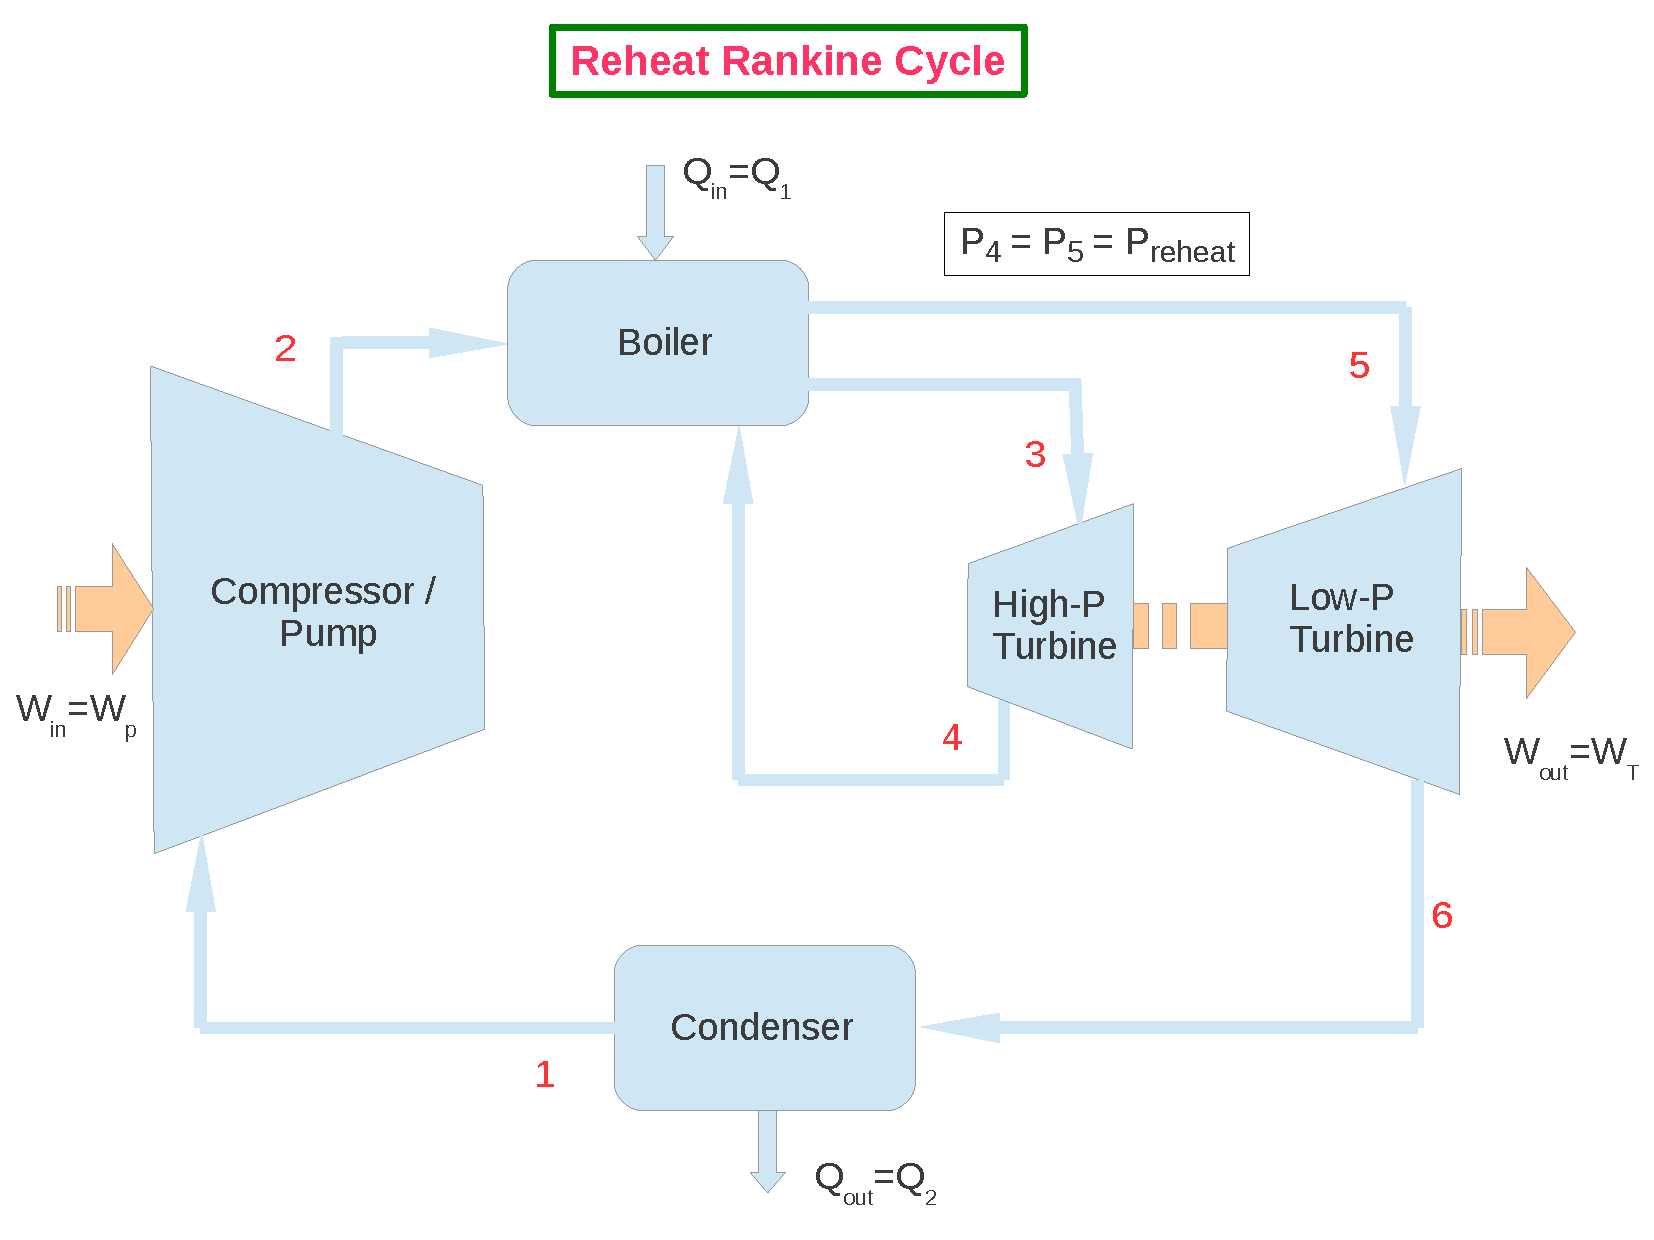
\includegraphics[width=6.25cm,clip]{./Pics/Reheat_Rankine_Cycle}
          \end{figure}
       \end{center}
       \begin{enumerate}[(a)] \scriptsize\setcounter{enumi}{6}
          \item<1-> Total heat input: 
              \visible<1->{\begin{eqnarray}
                  \blue{Q_{\text{total}}}&=& Q_{\text{primary}} + Q_{\text{reheat}} \nonumber \\
                                    &=& \blue{\left(h_{1}-h_{6}\right)+\left(h_{3}-h_{2}\right)}
              \end{eqnarray}}
       \end{enumerate}
     \end{column}
     \begin{column}[c]{0.5\linewidth}
       \begin{center}
          \begin{figure}
             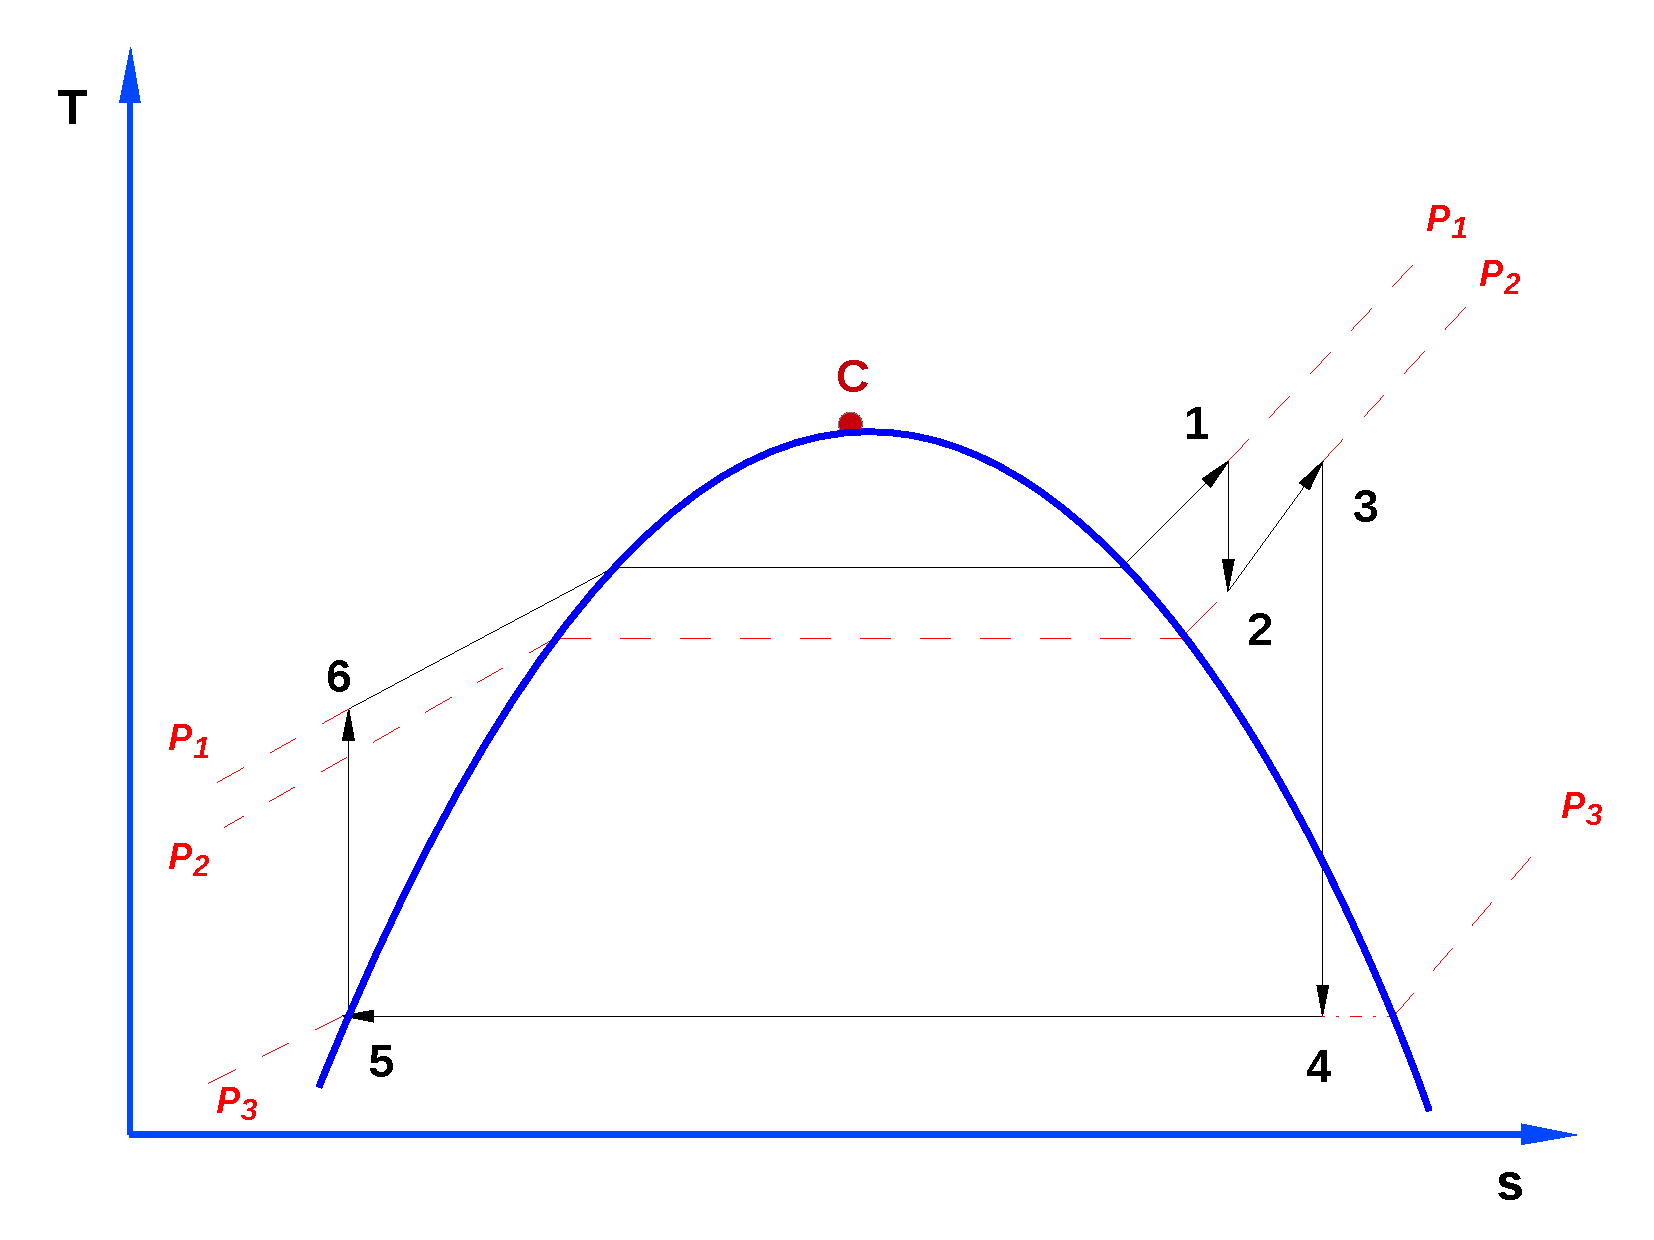
\includegraphics[width=6.25cm,clip]{./Pics/Reheat_Rankine_Cycle_Diagram2}
          \end{figure}
       \end{center}
       \begin{enumerate}[(a)] \scriptsize\setcounter{enumi}{7}
          \item<2-> Total turbine work output:
              \visible<2->{\begin{eqnarray}
                  \blue{W_{\text{turbine}}^{\text{total}}} &=& W_{\text{turbine}}^{\text{high-P}} + W_{\text{turbine}}^{\text{low-P}} \nonumber \\
                                                      &=& \blue{\left(h_{2}-h_{1}\right)+\left(h_{4}-h_{3}\right)}
              \end{eqnarray}}
       \end{enumerate}
     \end{column}
  \end{columns}
 \normalsize
\end{frame}

%%%
%%% SUBSECTION
%%%
\subsection{Regenerative Rankine Cycle}

%%%
%%% Slide
%%%
\begin{frame}
 \frametitle{Ideal Regenerative Rankine Cycle (Open feedwater heater)}
  \begin{columns}
    \begin{column}[c]{0.5\linewidth}
      \begin{enumerate}[(a)]\scriptsize
         \item<1-> In simple RC the \blue{temperature of the working fluid entering the boiler is substantially lower than the boiler steam exiting temperature}.  This results in \red{lower thermal efficiency};
         \item<2-> In the \blue{Regenerative Rankine Cycle} the temperature of the fluid leaving the pump ({\it feedwater}) is raised in several stages using steam extracted from the turbine;
         \item<3-> The device where the feedwater is heated by regeneration is called a \blue{regenerator} or \blue{feedwater heater (FWH)};
     %\item <4-> Not only improve thermal efficiency but also deaerates the feedwater that helps prevent corrosion and pump cavitation;
         \item<4-> A FWH is a heat exchanger where heat is transferred from the steam to the feedwater either by mixing the two fluid streams (\blue{open feedwater heaters}) or without mixing them (\blue{closed feedwater heaters}).
    \end{enumerate} 
   \end{column}
   \begin{column}[c]{0.5\linewidth} 
     \begin{center}
        \begin{figure}
            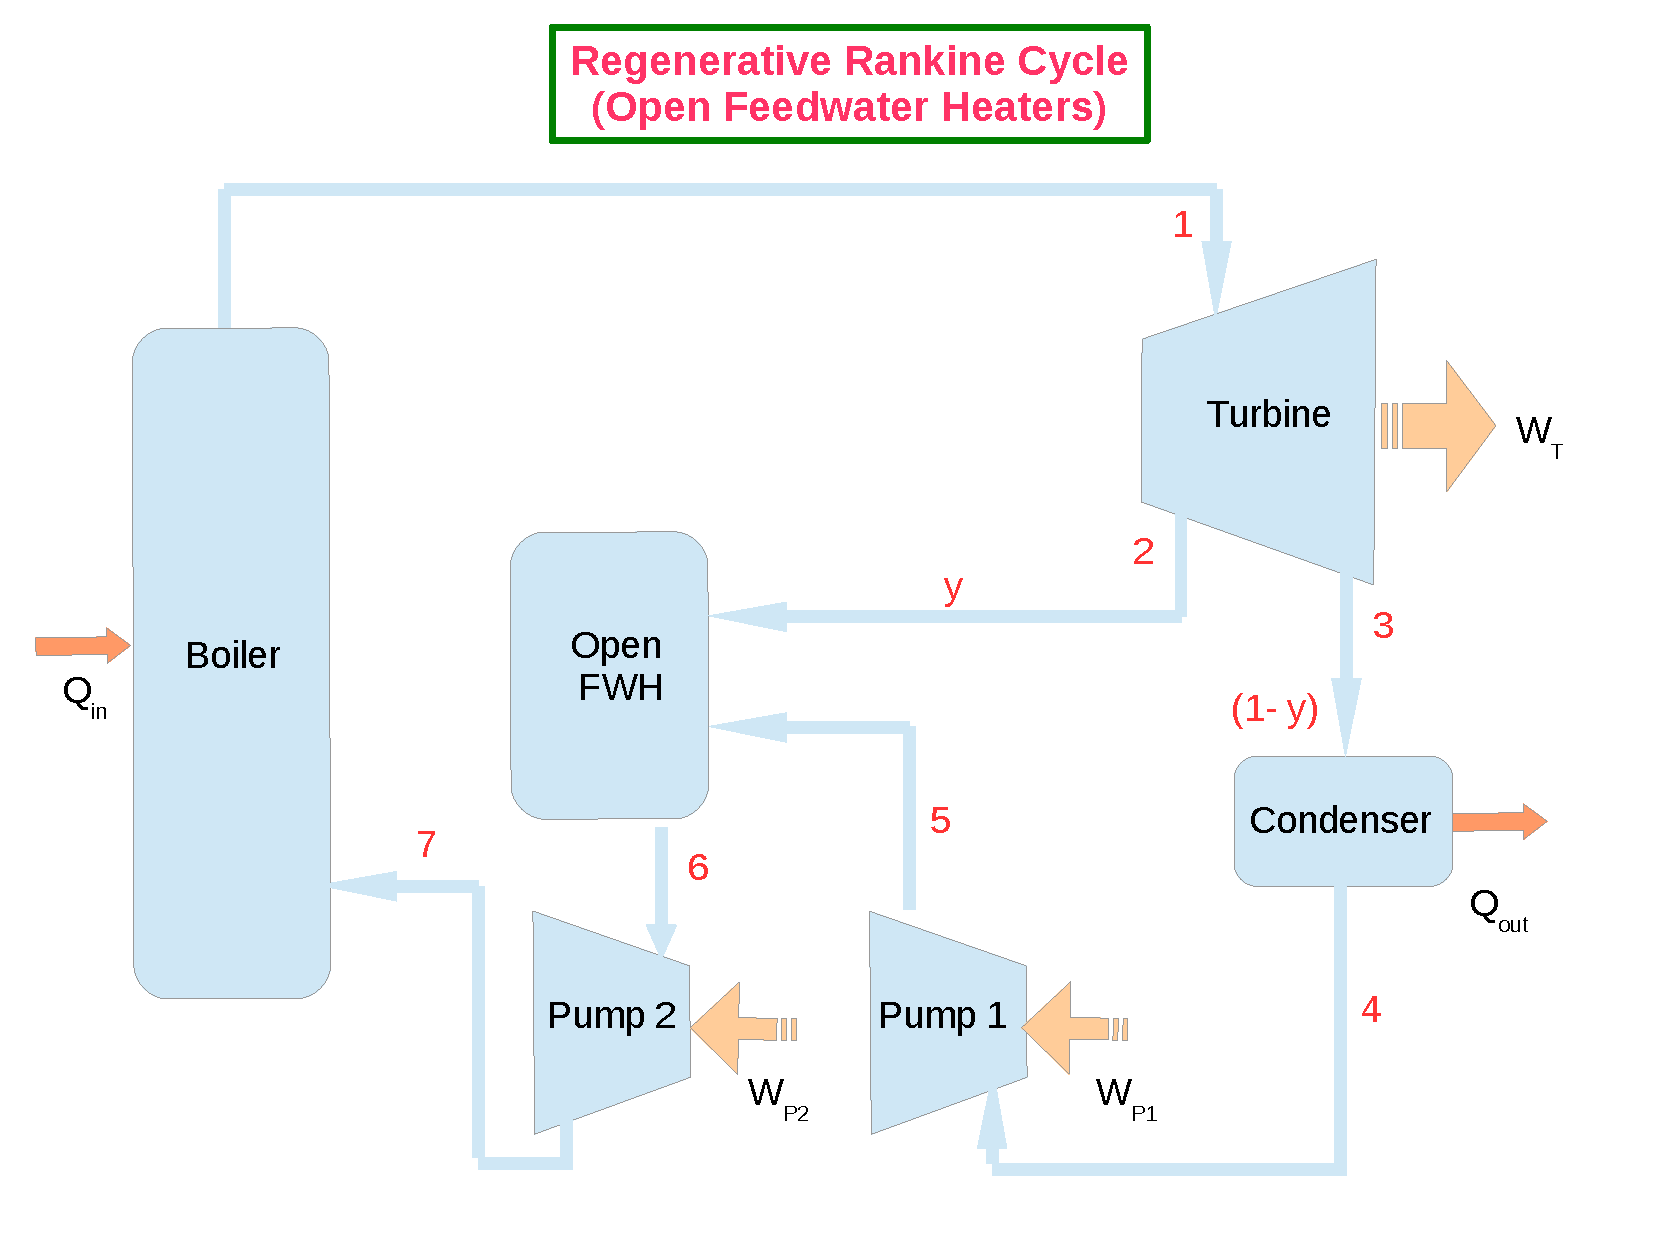
\includegraphics[width=6.5cm,clip]{./Pics/RegenerativeOpen_RankineCycle}
        \end{figure}
     \end{center}
   \end{column}
  \end{columns}
 \normalsize
\end{frame}


%%%
%%% Slide
%%%
\begin{frame}
 \frametitle{Ideal Regenerative Rankine Cycle (Open feedwater heater)}
  \begin{columns}
    \begin{column}[c]{0.5\linewidth}
     \begin{center}
        \begin{figure}
            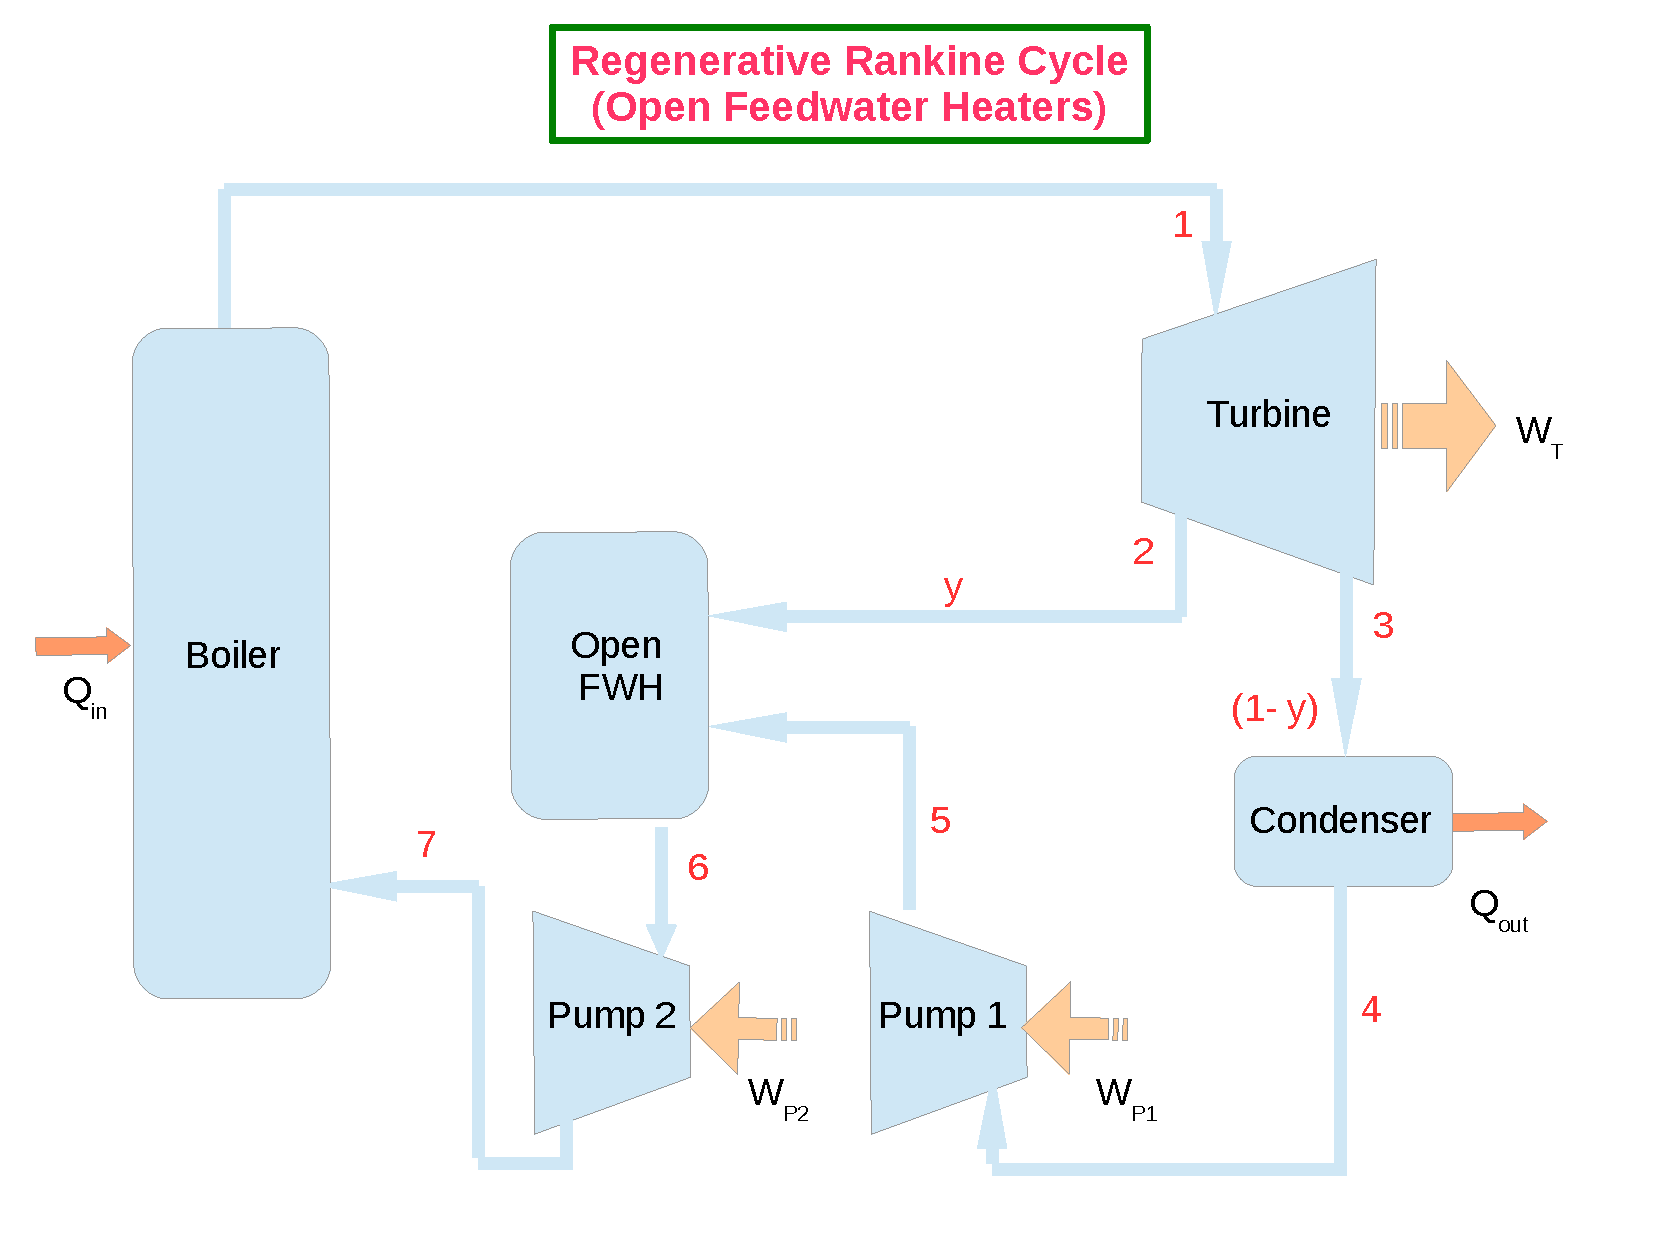
\includegraphics[width=5.5cm,clip]{./Pics/RegenerativeOpen_RankineCycle}
        \end{figure}
     \end{center}
     \begin{enumerate}[(a)]\setcounter{enumi}{4}\scriptsize
         \item<1->  A fraction of the steam extracted from the turbine \blue{($y$)} leaves the FWH as {\it saturated liquid} $\left(P_{\text{FWH}}\right)$, and a second pump raises the pressure to $P_{\text{boiler}}$;
         \item<2-> Heat balance in the cycle:
             \visible<2->{\begin{eqnarray}
                && \blue{Q_{\text{in}} = H_{1}-H_{7}} \\
                && \blue{Q_{\text{out}} = \left(1 - y \right)\left(H_{4} - H_{3}\right)} 
             \end{eqnarray}}
     \end{enumerate}
   \end{column}
    \begin{column}[c]{0.5\linewidth}
     \begin{center}
        \begin{figure}
            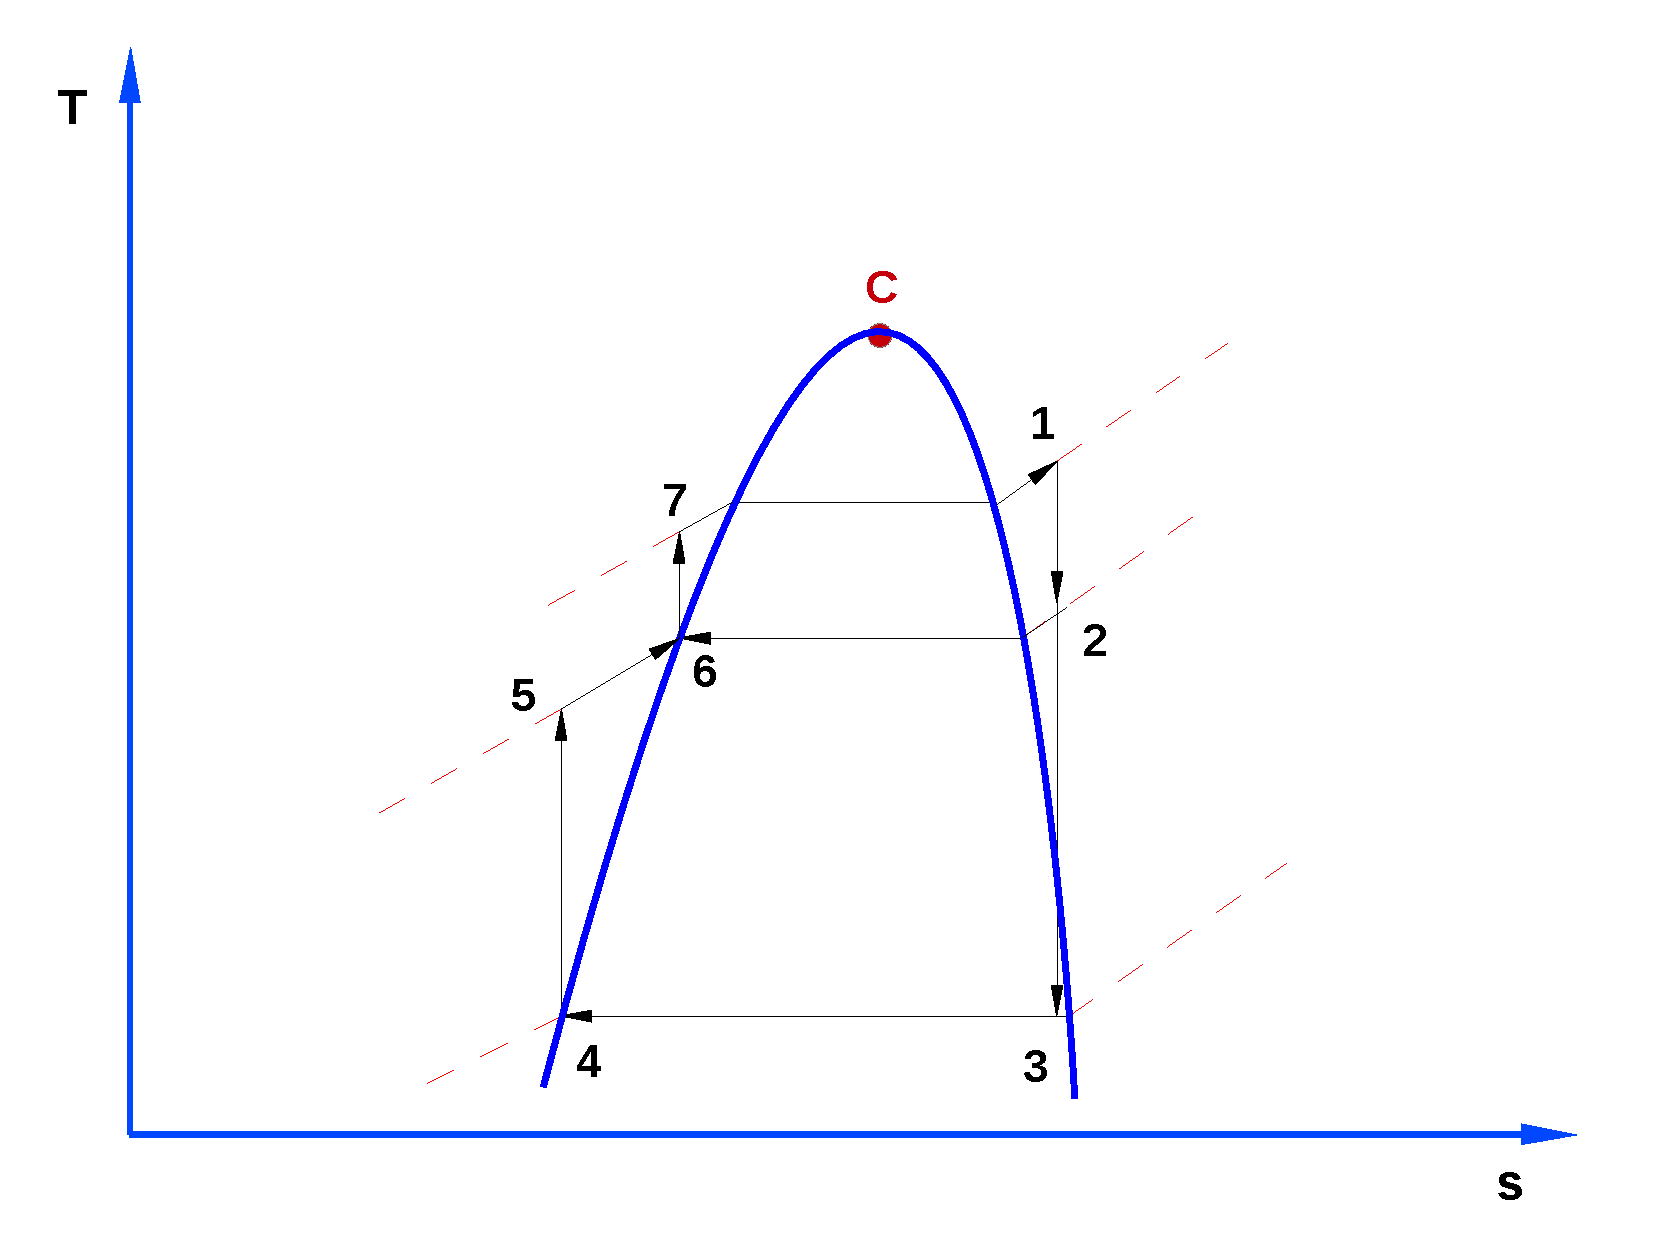
\includegraphics[width=6.cm,clip]{./Pics/RegenerativeOpen_RankineCycle_Diagram}
        \end{figure}
     \end{center}
     \begin{enumerate}[(a)]\setcounter{enumi}{6}\scriptsize
         \item<3-> Pump and turbine work:
             \visible<3->{\begin{eqnarray}
                \blue{W_{\text{Turbine}}^{\text{out}} = \left[y h_{2} + \left(1-y\right)h_{3}\right]-h_{1}}\\ 
                \blue{W_{\text{Pump}}^{\text{in}} = \left(1 - y \right) W_{\text{Pump,1}}^{\text{in}} + W_{\text{Pump,2}}^{\text{in}}}
             \end{eqnarray}}
     \end{enumerate}
   \end{column}
  \end{columns}
 \normalsize
\end{frame}

%%%
%%% Slide
%%%
\begin{frame}
 \frametitle{Ideal Regenerative Rankine Cycle (Closed feedwater heater)}
  \begin{columns}
    \begin{column}[c]{0.5\linewidth}
     \begin{center}
        \begin{figure}
            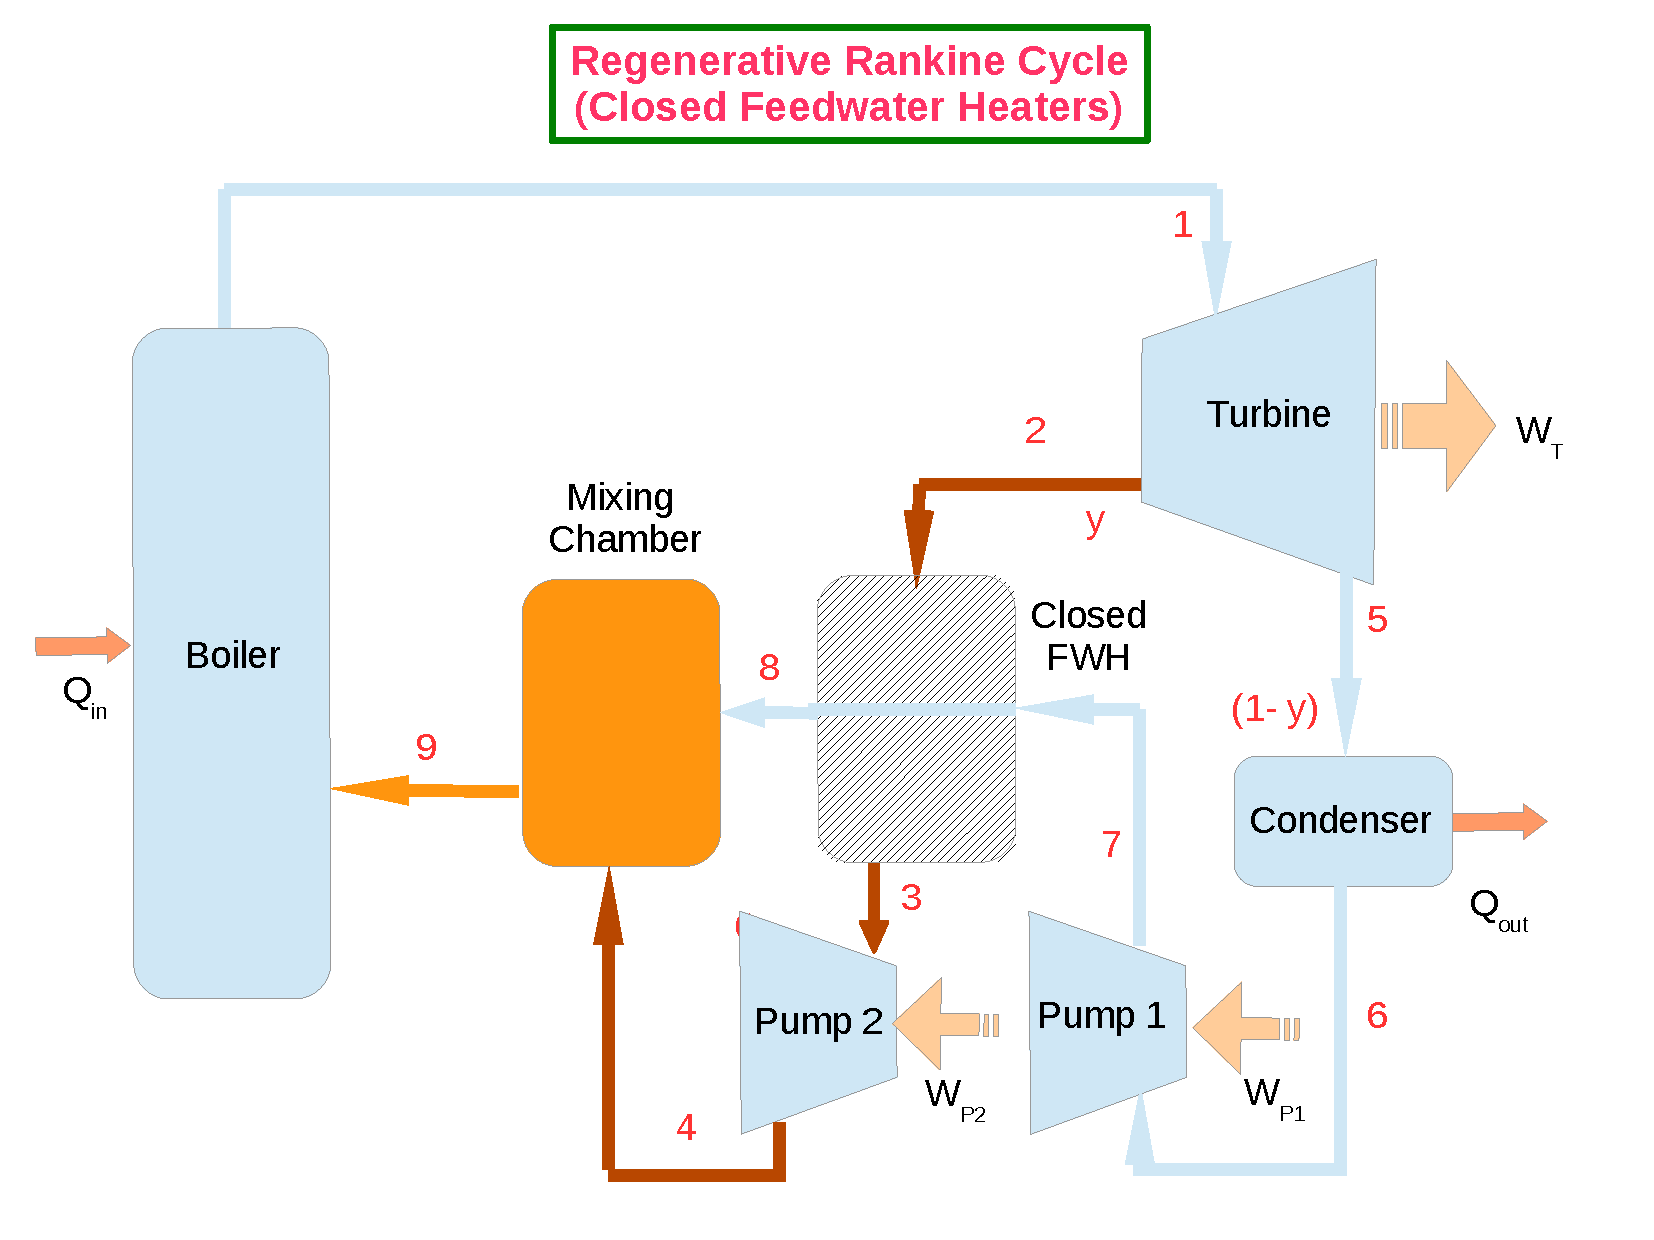
\includegraphics[width=6.cm,clip]{./Pics/RegenerativeClosed_RankineCycle}
        \end{figure}
     \end{center}
   \end{column}
    \begin{column}[c]{0.5\linewidth}
     \begin{center}
        \begin{figure}
            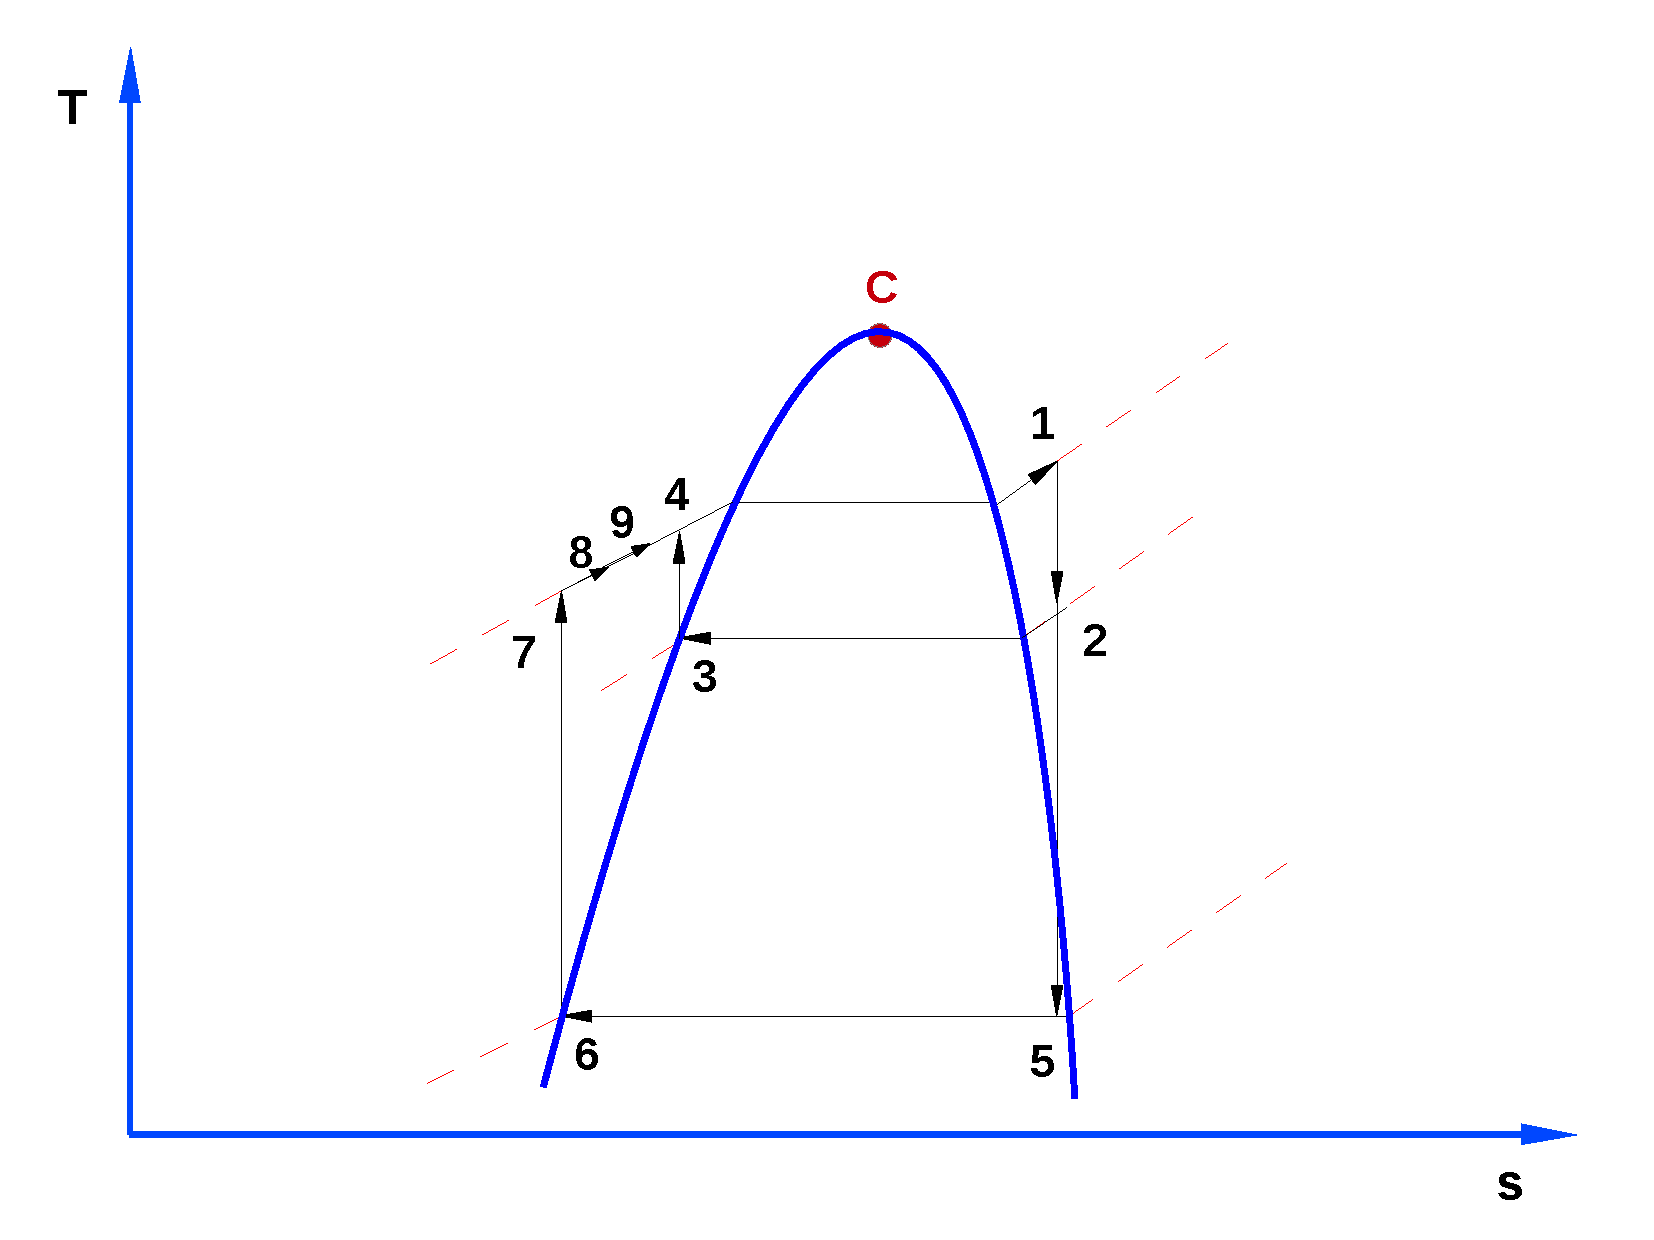
\includegraphics[width=6.25cm,clip]{./Pics/RegenerativeClosed_RankineCycle_Diagram}
        \end{figure}
     \end{center}
   \end{column}
  \end{columns}
 \normalsize
\end{frame}


%%%
%%% Slide
%%%
\begin{frame}
 \frametitle{Regenerative $\times$ Simple Rankine Cycles}
  \begin{columns}
   \begin{column}[c]{0.5\linewidth}
    \begin{enumerate}[(a)]
     \item<1-> Advantages of Regenerative cycle over Simple Rankine Cycle
     \begin{enumerate} [(i)]%\scriptsize
      \item<1-> The heating process in the boiler tends to become reversible;
      \item<1-> Thermal stresses in boiler are minimised due to the smaller temperature ranges in the boiler;
      \item<1-> Thermal efficiency is improved as the average temperature of heat addition to the cycle is increased;
      \item<1-> Due to continuous steam extraction, the content of moisture is reduced and this decreases the corrosion in the turbine;
      \item<1-> The size of the condenser is smaller (lower cost and better maintenance).
     \end{enumerate}
    \end{enumerate} 
   \end{column}
%
   \begin{column}[c]{0.5\linewidth}  
    \begin{enumerate}[(a)]\setcounter{enumi}{1}
     \item<2-> Disadvantages of Regenerative cycle over Simple Rankine Cycle
     \begin{enumerate}[(i)] %\scriptsize
      \item<2-> Design of the power plant is more complex;
      \item<2-> As the number of heaters is increased, the greater maintenance (larger cost) is required;
      \item<2-> Heater are usually costly and the gain in thermal efficiency may not be enough. 
     \end{enumerate}
    \end{enumerate} 
   \end{column}
  \end{columns}
  
\end{frame}
 















































%%%%%%%%%%%%%%%%%%%%%%%%%%%%%%%%%%%%%%%%%%%%%%%%%%%%%%%%%%%%%%%%%%%%%%%%%%%%%%%%%%%%%%%%%%%%%%%%%%%%%%%%%%%%%

%%%
%%% Slide
%%%
\begin{frame}
 \frametitle{Example 1: Simple Steam Power Plant}
 %\scriptsize
    {\it The table below represents the steps of an idealised steam power plant with
    \begin{center}
     \begin{tabular}{||c | c | c | c | c ||}
      \hline\hline
       {\bf Step} & {\bf Location}       & {\bf Pressure}  & {\bf Temperature /}   & {\bf Velocity} \\
                  &                      & {\bf (bar)}     & {\bf Quality}         & {\bf m/s}      \\
      \hline\hline
          1       & Inlet to turbine     &   60            &   380 $^{o}$C          &   --           \\
      \hline
          2       & Exit from turbine and&   0.1           &   0.9                 & 200             \\
                  & inlet to condenser   &                 &    --                 &     --          \\ 
      \hline
          3       & Exit from condenser and&  0.09         &  Saturated            &   --            \\
                  & inlet to pump        &                 &  Liquid               &                 \\
      \hline
          4       & Exit from pump and   &  70             &   --                  &     --          \\
                  & inlet to boiler      &                 &                       &                 \\
      \hline 
          5       & Exit from boiler     &  65             &  400 $^{o}$C           &      --        \\
                  & Rate of steam flow:   &                 &                       &                 \\
                  & 1.0$\times$10$^{4}$ kg/h &             &                       &                 \\
     
      \hline\hline
     \end{tabular}
    \end{center}}
 \normalsize
\end{frame}


%%%
%%% Slide
%%%
\begin{frame}
 \frametitle{Example 1: Simple Steam Power Plant}
 %\scriptsize
    {\it Calculate:
    \begin{enumerate}[(a)]
     \item Power output of the turbine.
     \item Heat transfer per hour in the boiler and condenser.
     \item Mass rate of cooling water circulated (kg/h) in the condenser assuming inlet and outlet fluid temperatures from the condenser of 20$ ^{o}$C and 30 $^{o}$C.
     \item Diameter of the pipe connecting the turbine with the condenser. 
    \end{enumerate}}
 \normalsize
\end{frame}



%%%
%%% Slide
%%%
\begin{frame}
 \frametitle{Example 1: Simple Steam Power Plant}
     
\begin{center}
       \begin{tabular}{|c c c c c|}
         \hline
          P(bar) /   &      &   300       &  350     &  400 \\
          T($^{o}$C) &       &             &         &      \\
          \hline
             60     &  $h$ (kJ/kg)   &   2884.2   & 3043.0   &  3177.2 \\
          \hline
       \end{tabular} 
\end{center}

    \begin{figure}%
     \begin{center}
      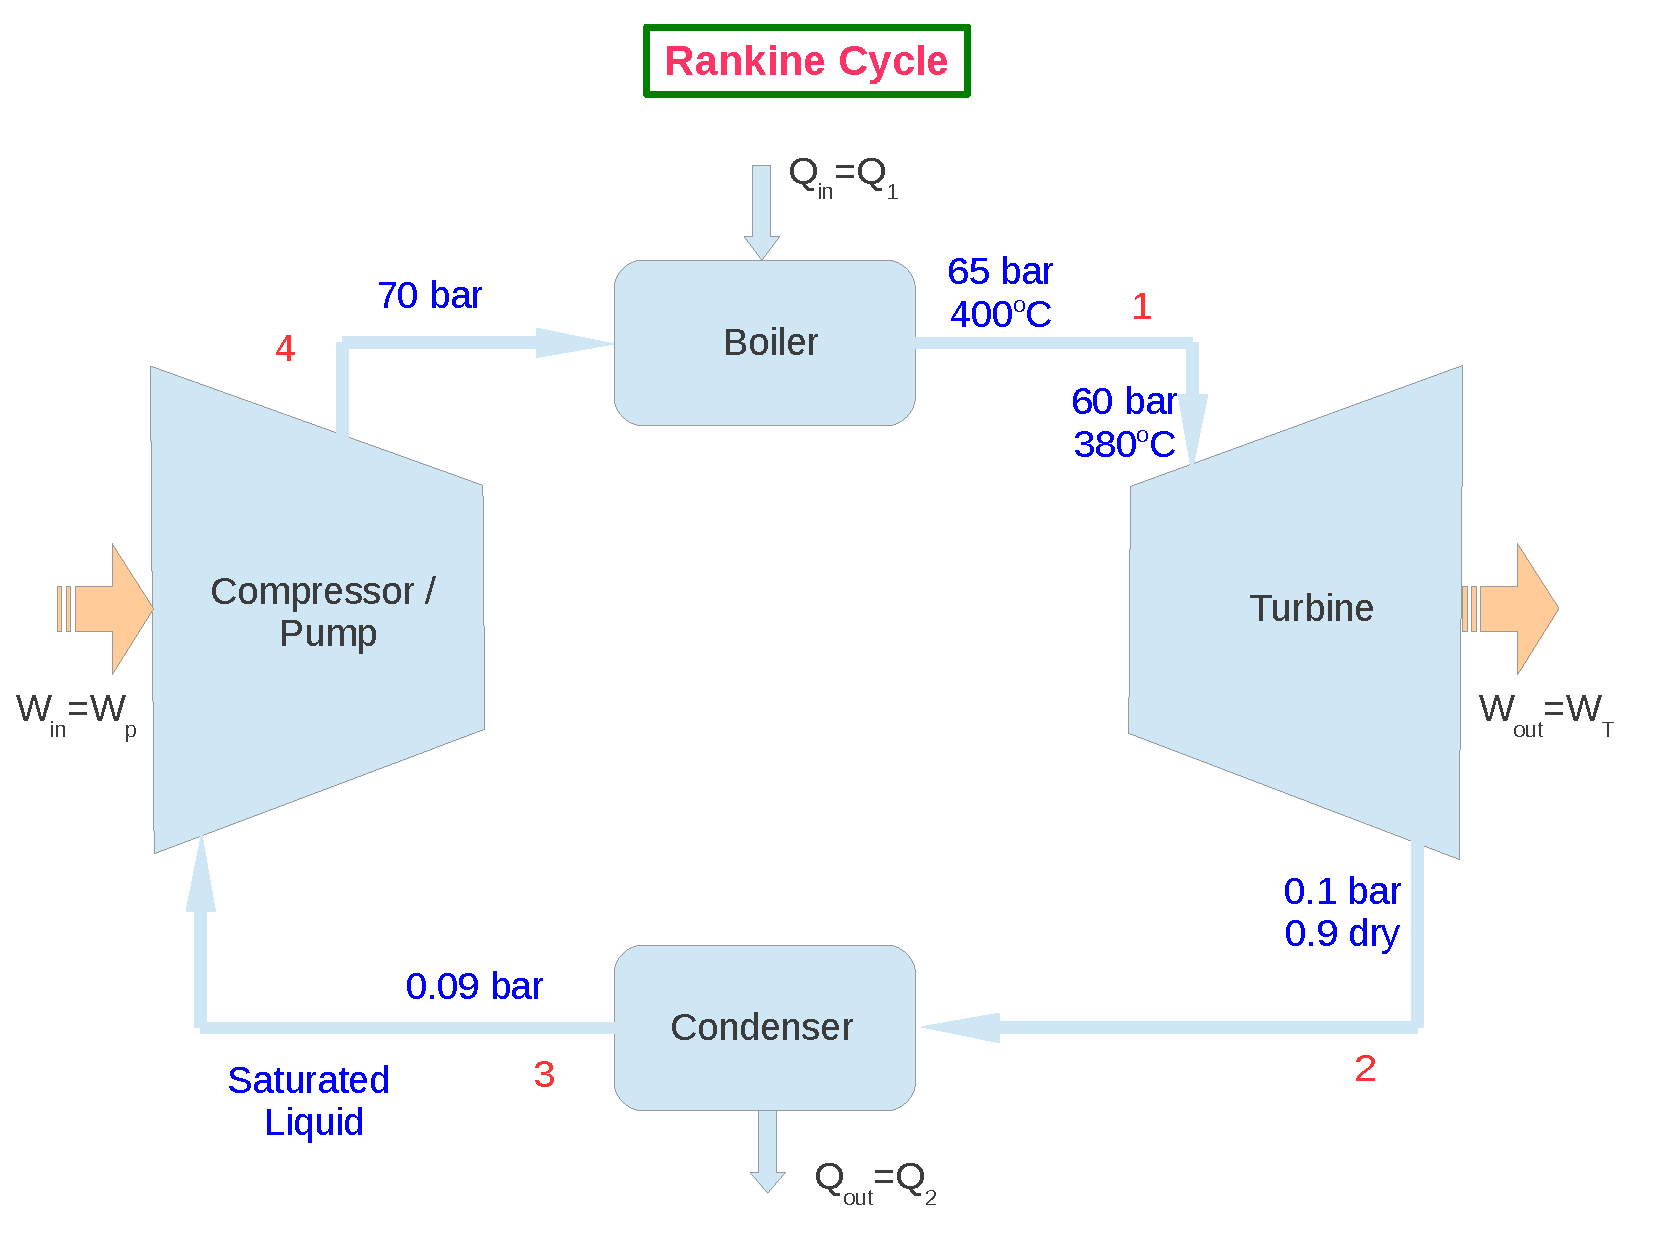
\includegraphics[width=7.5cm,clip]{./Pics/Rankine_Cycle_Exemple01}
     \end{center}
    \end{figure} 


 \normalsize
\end{frame}



%%%
%%% Slide
%%%
\begin{frame}
 \frametitle{Example 1: Simple Steam Power Plant}

    \textcolor{blue}{(a) Power output of the turbine:} From superheated steam table at 60 bar (above), the enthalpy at 380 $^{o}$C is calculated via linear interpolation:\\
        $h_{1}=3043.0 + \displaystyle\frac{3177.2-3043.0}{400-350}\left(380.0-350.0\right)$\\
        $h_{1}=3123.5\;\;kJ/kg$ \\
 
    The pressure at the output from the turbine is 0.1 bar and the enthalpies are:\\
\begin{center}
    \begin{tabular}{|c c c c c|}
     \hline
     P    & T$_{S}$  & h$_{f}$  & h$_{fg}$ & h$_{g}$ \\
    (bar) & ($^{o}$C) & (kJ/kg) & (kJ/kg) & (kJ/kg) \\
    \hline
     0.1 &  45.8     & 191.8   & 2392.8  & 2584.7 \\
    \hline 
    \end{tabular}
\end{center}

    with $x_{2}=0.9$. Thus:\\
    $h_{2}=h_{f_{2}}+x_{2}h_{fg_{2}} = 191.8 + 0.9\times 2392.8$\\
    $h_{2}=2345.3 kJ/kg$\\
    And the power output of the turbine, $P_{T}$ (assuming rate of steam flow on 10000 kg/h:\\
    $P_{T}=m_{s}\left(h_{1}-h_{2}\right)=\displaystyle\frac{1.0\times 10^{4}}{3600}\left(3123.5-2345.3\right)$\\
    \textcolor{blue}{$P_{T}=2162 kW$}

 \normalsize
\end{frame}



%%%
%%% Slide
%%%
\begin{frame}
 \frametitle{Example 1: Simple Steam Power Plant}
 %\scriptsize
    {\it 
    \textcolor{blue}{(b) Heat transfer (per hour) in the boiler $\&$ condenser:} the fluid enters in the boiler at 70 bar $\left(h_{f_{4}}=1267.4\;kJ/kg\right)$ and leaves at 65 bar $\left(T=400^{o}C\right)$ with the enthalpy calculated via linear interpolation of the superheated steam enthalpies at 60 and 70 bars:}\\
\medskip
$h_{\text{out}}^{\text{boiler}}=\displaystyle\frac{3177.2-3158.1}{2}=3167.6\;kJ/kg$\\
The heat transfer in the boiler is, \\
$Q_{1}=m_{s}\left(h_{\text{out}}^{\text{boiler}}-h_{4}\right)=10^{4}\times\left(3167.65-1267.4\right)=1.9\times 10^{7}\;kJ/kg$
\\
\medskip
Now, the heat transfer in the condenser is,\\
\medskip
$Q_{2}=m_{s}\left(h_{2}-h_{3}\right)=10^{4}\times\left(2345.3-183.3\right)=2.16\times 10^{7}\; kJ/h$\\
\medskip

\textcolor{blue}{(c) Mass of cooling water circulated (per hour) in the condenser, $m_{w}$:} The heat lost by the steam is fully transferred to the cooling water,\\
\medskip 
$Q_{2}=m_{w}C_{p,w}\left(T_{2}-T_{1}\right)$\\
\medskip
$2.16\times 10^{7} = m_{w}\times 4.18\left(30-20\right)$\\
\medskip
\textcolor{blue}{$m_{w}=5.17\times 10^{5}\;kg/h$}


 \normalsize
\end{frame}



%%%
%%% Slide
%%%
\begin{frame}
 \frametitle{Example 1: Simple Steam Power Plant}
 %\scriptsize
  \begin{columns}
   \begin{column}[c]{0.5\linewidth}
    {\it  
    \textcolor{blue}{(d) Diameter $\left(\phi\right)$ of the pipe connecting the turbine and the condenser:}\\
$\displaystyle\frac{\pi}{4}\phi^{2}u_{s}=m_{s}x_{2}v_{g_{2}}$\\
where $u_{s}$ and $v_{g_{2}}$ are the steam velocity (=200 m/s) and the specific volume at 0.1 bar $\left(=14.67\;m^{3}/kg\right)$, respectively. Substituting the values in the expression above,\\
\textcolor{blue}{$\phi=0.483\;m$}
}
   \end{column}

   \begin{column}[c]{0.5\linewidth}
    \begin{figure}%
     \begin{center}
      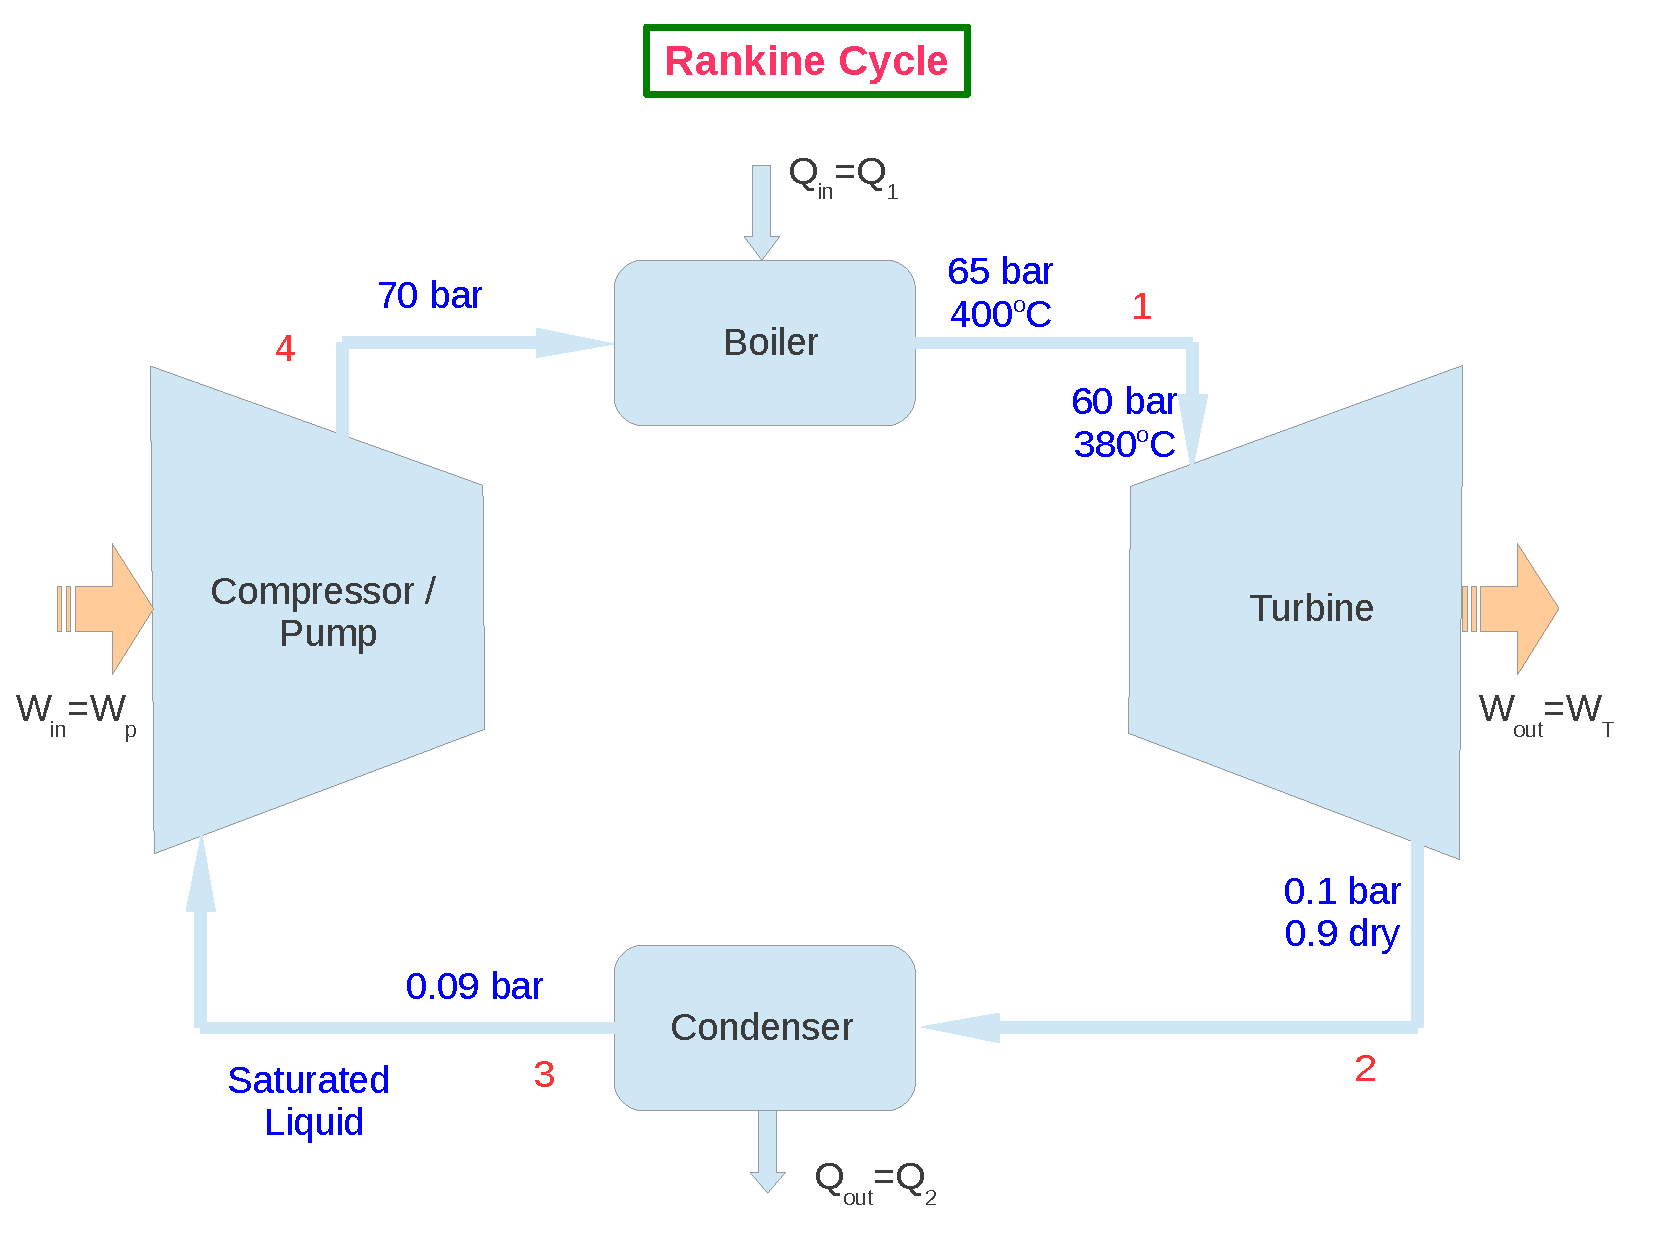
\includegraphics[width=6.25cm,clip]{./Pics/Rankine_Cycle_Exemple01}
     \end{center}
    \end{figure}  
   \end{column}
  \end{columns}

 \normalsize
\end{frame}




\subsection{Modified Rankine Cycles}
%%%
%%% Slide
%%%
\begin{frame}
 \frametitle{The Ideal Reheat Rankine Cycle}
  \begin{columns}
   \begin{column}[c]{0.5\linewidth}

 \begin{itemize} %\scriptsize
  \item <1-> Thermal efficiency can be enhanced by increasing the boiler pressure;
  \item <2-> However, this results in higher moisture content in the steam flow which can damage the turbine;
 \end{itemize}
   \end{column}

   \begin{column}[c]{0.5\linewidth} 
    \begin{figure}%
     \begin{center}
      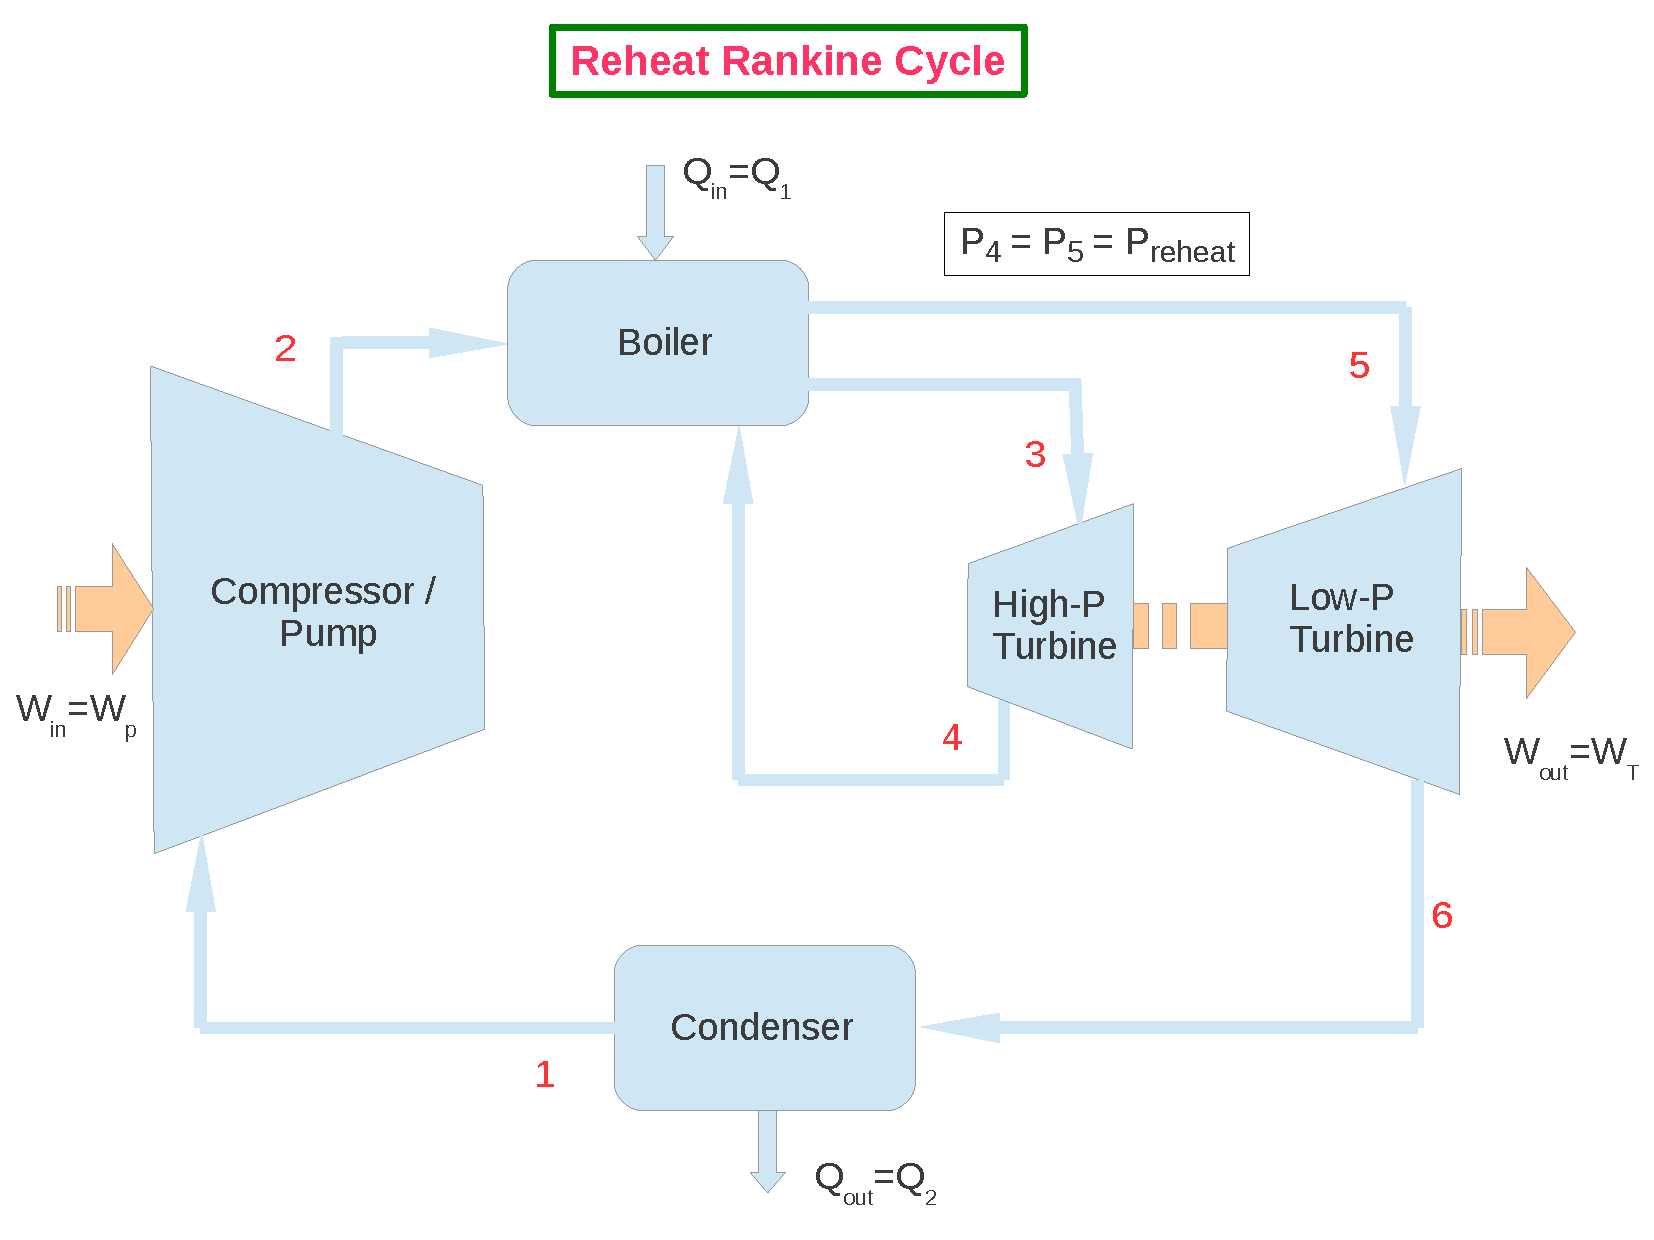
\includegraphics[width=6.25cm,clip]{./Pics/Reheat_Rankine_Cycle}
     \end{center}
    \end{figure}  
   \end{column}
  \end{columns}
 \normalsize
\end{frame}



%%%
%%% Slide
%%%
\begin{frame}
 \frametitle{The Ideal Reheat Rankine Cycle}
  \begin{columns}
   \begin{column}[c]{0.5\linewidth}

 \begin{itemize} %\scriptsize
  \item <1-> To overcome this problem we may:
  \begin{enumerate}[(a)] %\scriptsize
   \item <2-> Superheat the steam before the turbine: this would improve thermal efficiency of the cycle but the very high temperature may be prohibitive as novel (and more expansive) material would need to be used;
   \item <3-> Expand the steam in the turbine in two stages and reheat in between. This is an improvement on the ideal Rankine cycle as we would add a reheating process between continuous expansion.
  \end{enumerate} 
 \end{itemize}
   \end{column}

   \begin{column}[c]{0.5\linewidth} 
    \begin{figure}%
     \begin{center}
      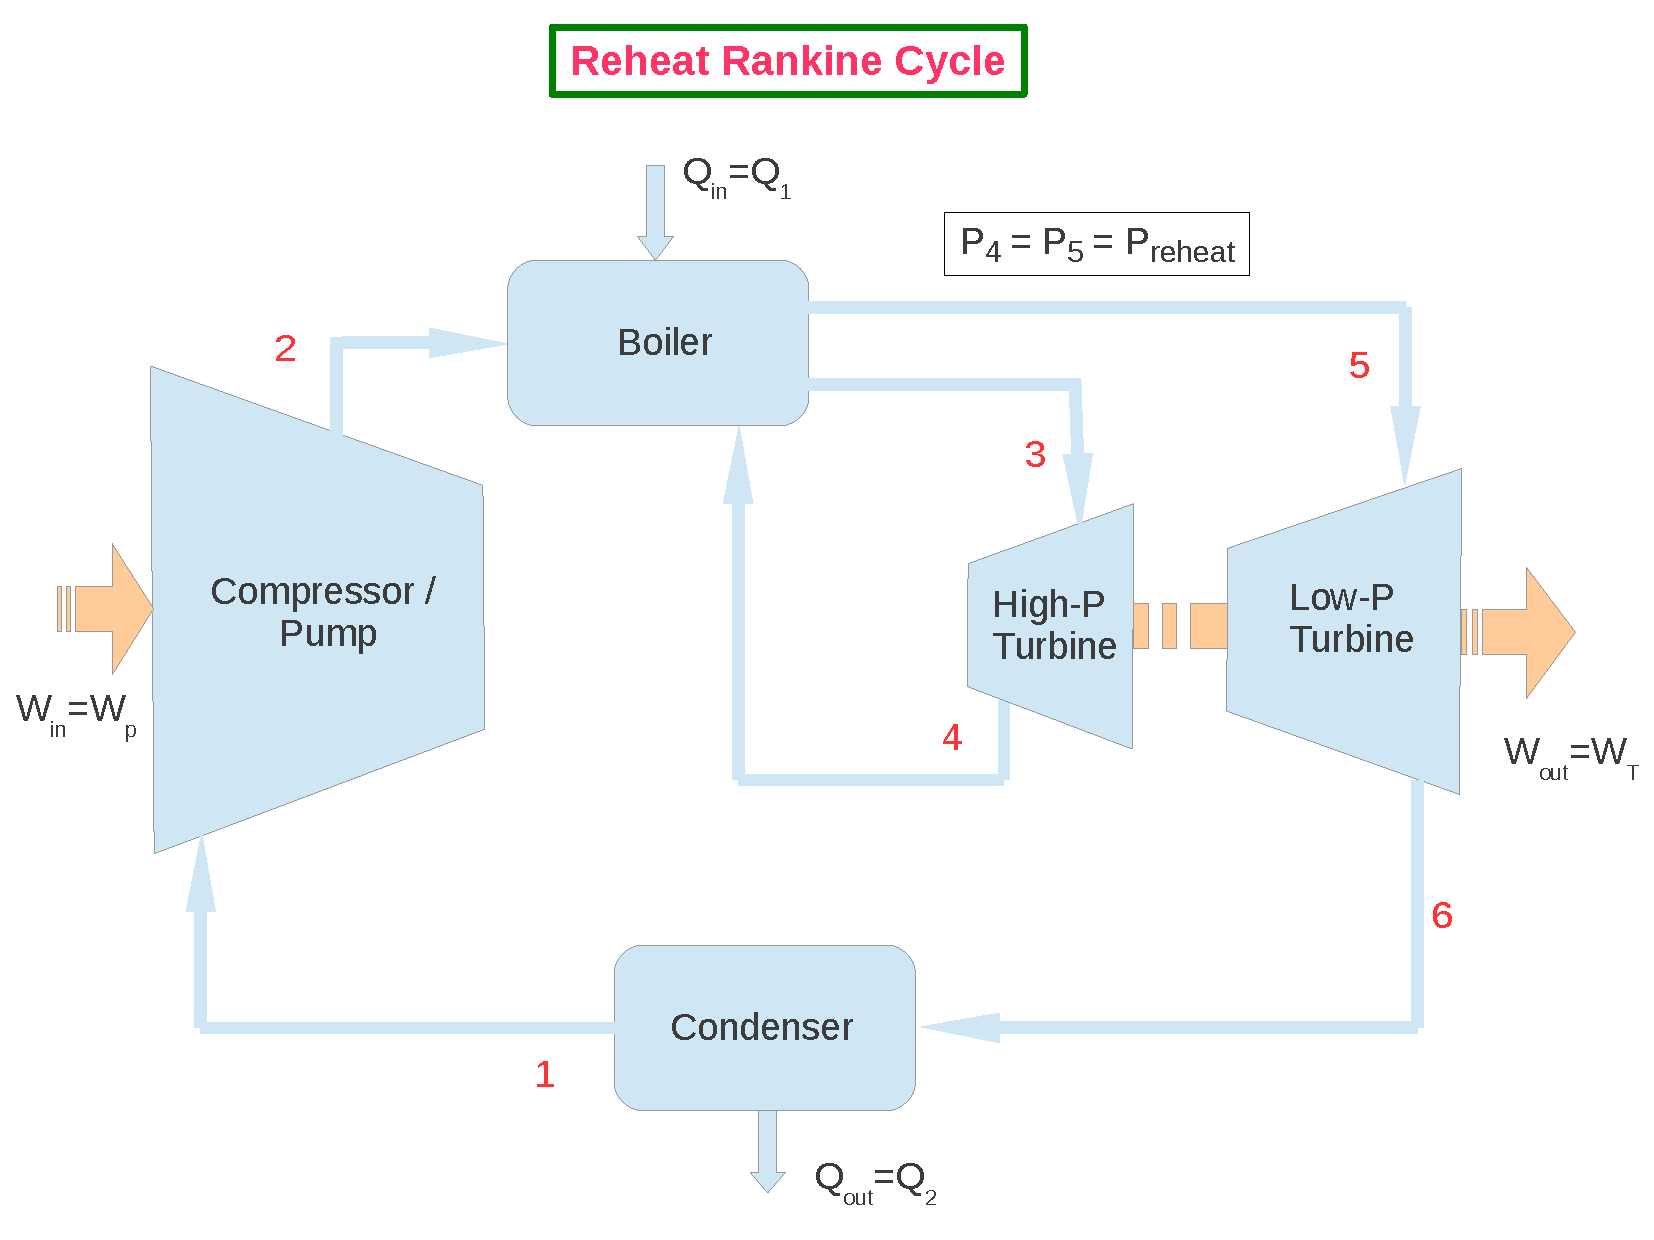
\includegraphics[width=6.25cm,clip]{./Pics/Reheat_Rankine_Cycle}
     \end{center}
    \end{figure}  
   \end{column}
  \end{columns}
 \normalsize
\end{frame}





%%%
%%% Slide
%%%
\begin{frame}
 \frametitle{The Ideal Reheat Rankine Cycle}
  \begin{columns}
   \begin{column}[c]{0.5\linewidth}

 \begin{itemize} %\scriptsize
  \item <1-> Expansion occurs in a 2-stages process:
  \begin{enumerate}[(a)] %\scriptsize
   \item <2-> {\it First Stage (High-P Turbine):} steam is expanded isentropically to an intermediate pressure and return to the boiler where it is reheated at constant pressure;
   \item <3-> {\it Second Stage (Low-P Turbine:} steam is expanded isentropically to the condenser pressure;
  \end{enumerate}
  \item <4-> Total heat input is $q_{\text{in}}=q_{\text{primary}}+q_{\text{reheat}}=$$\left(h_{3}-h_{2}\right)+\left(h_{5}-h_{4}\right)$;
  \item <5-> Total turbine work output is $W_{\text{turb}}^{\text{out}} = W_{\text{turb}}^{\text{high-P}} + W_{\text{turb}}^{\text{low-P}}=$ $\left(h_{3}-h_{4}\right)+\left(h_{5}-h_{6}\right)$
 \end{itemize} 
   \end{column}

   \begin{column}[c]{0.5\linewidth} 
    \begin{figure}%
     \begin{center}
      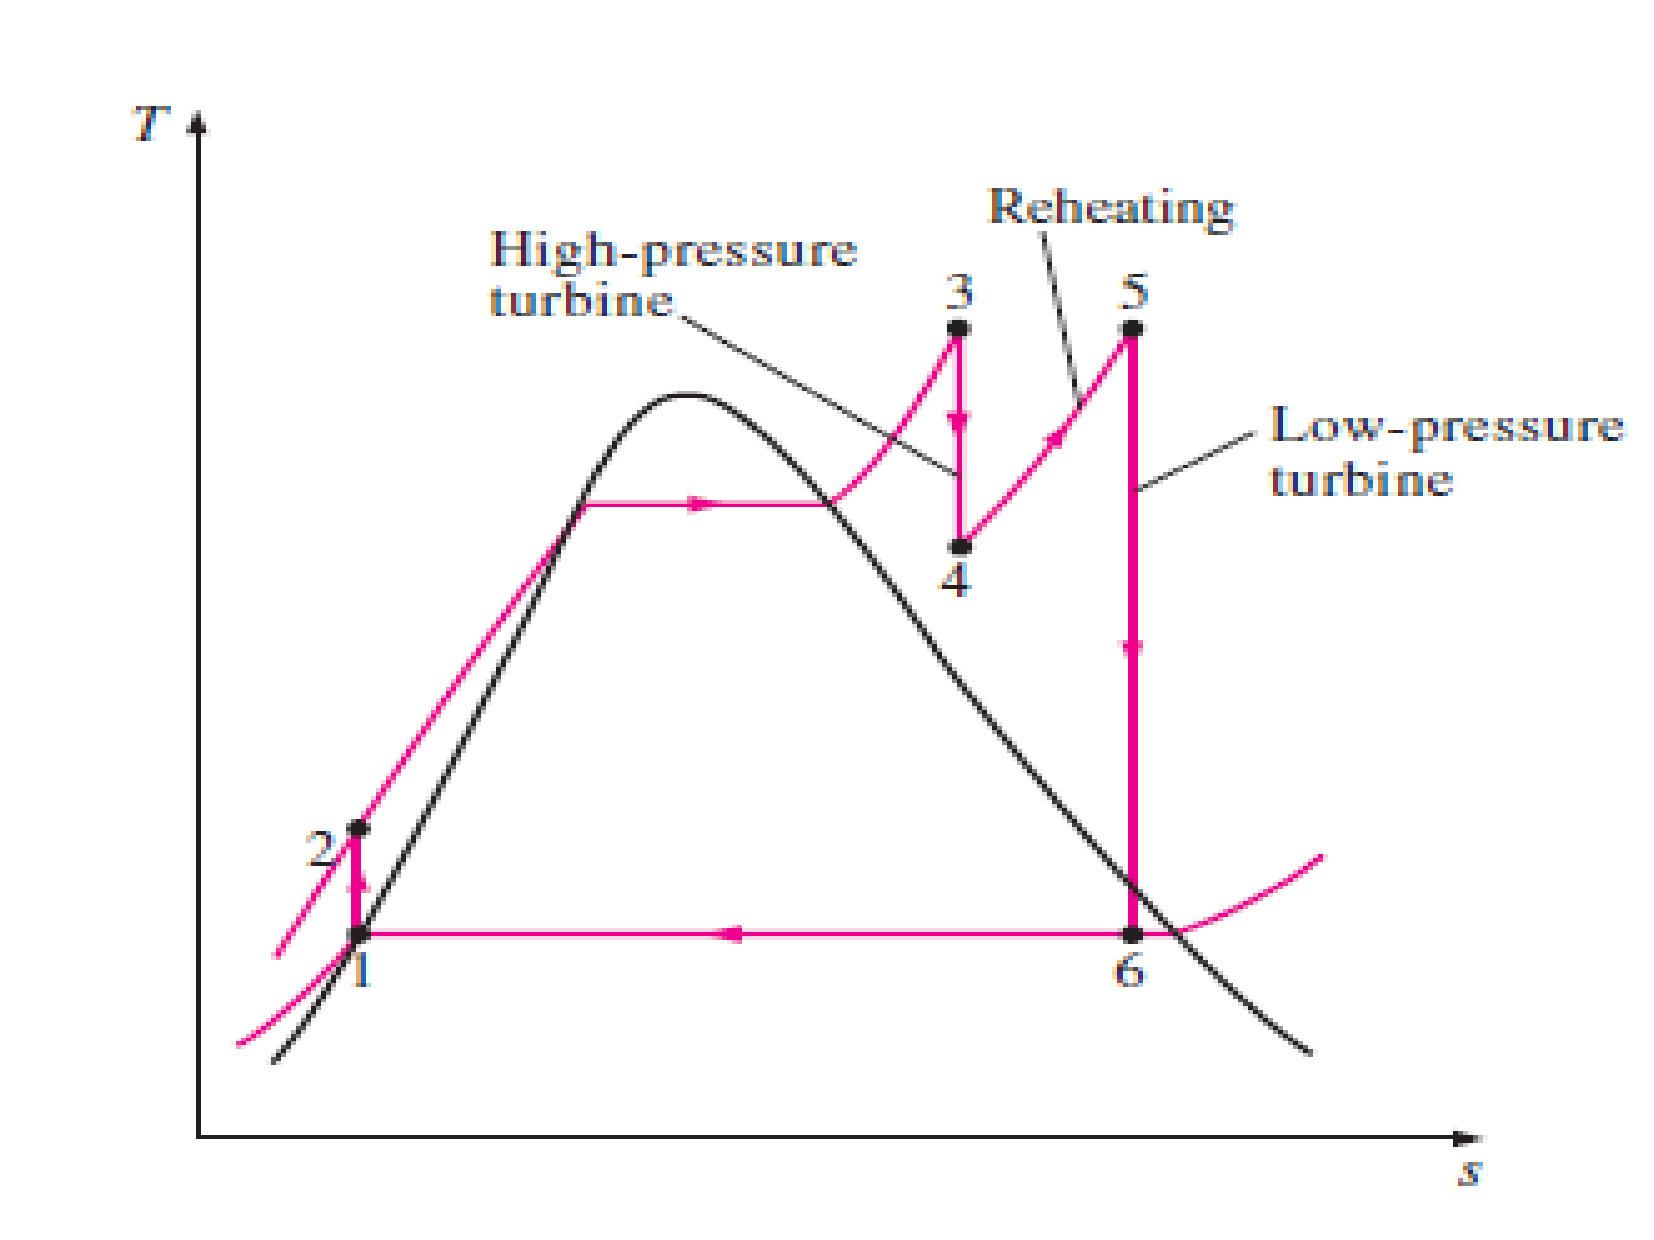
\includegraphics[width=6.25cm,clip]{./Pics/Reheat_Rankine_Cycle_Diagram}
     \end{center}
    \end{figure}  
   \end{column}
  \end{columns}

 %\scriptsize
 \normalsize
\end{frame}



%%%
%%% Slide
%%%
\begin{frame}
 \frametitle{Advantages of Reheat Rankine Cycle}
  \begin{itemize}
   \item <1-> The main objective of using superheated steam is \textcolor{blue}{to avoid excessive moisture in the steam} at the end of the expansion process;
   \item <2-> A large moisture content in the steam would lead to larger condensation in the engine cyclinder, and it would result in blade erosion;
   \item <3-> Maximum moisture content of approx. 12$\%$ to avoid blades' damage;
   \item <4-> Thus superheated steam:
   \begin{enumerate}
    \item <5-> leads a reduction in the initial condensation losses in steam engines;
    \item <6-> improves the plant efficiency by saving fuel (costs).
    \item <7-> Reheating should be operated at \textcolor{blue}{optimum pressure};
    \item <8-> If the steam is reheated nearly in its expansion then the additional heat that need to be supplied will be small and the thermal efficiency gain will be small;
    \item <9-> If the reheating is operated at a fairly low pressure, then, although a large amount of additional heat is supplied, the steam will have a high degree of superheat (Mollier diagram), thus a large proportion of the heat supplied in the reheating process will be wasted in the condenser.
   \end{enumerate}
  \end{itemize}
 
\end{frame}


%%%
%%% Slide
%%%
\begin{frame}
 \frametitle{Advantages of Reheat Rankine Cycle}
 \begin{itemize}
  \item <1->\textcolor{blue}{Advantages of Reheating:}
   \begin{enumerate}
    \item <2-> There is an increased output from the turbine;
    \item <3-> Smaller problems -re to erosion and corrosion;
    \item <4-> Improvement of the thermal efficiency of the turbines;
    \item <5-> Smaller moisture content in the steam flow;
   \end{enumerate}
  \item <6->\textcolor{blue}{Disavantages of Reheating:}
   \begin{enumerate}
    \item <7-> Reheating requires more maintenance;
    \item <8-> Enhancement of thermal efficiency may not be enough to match the larger costs associated with reheating the steam.
   \end{enumerate}
 \end{itemize}
\end{frame}



%%%
%%% Slide
%%%
\begin{frame}
 \frametitle{Ideal Regenerative Rankine Cycle}
  \begin{columns}
   \begin{column}[c]{0.5\linewidth}
    \begin{enumerate} %\scriptsize
     \item <1-> In simple Rankine cycle the temperature of the working fluid entering the boiler is substantially lower than the boiler steam exiting temperature.  This results in lower thermal efficiency;
     \item <2-> In the {\it Regenerative Rankine Cycle} the temperature of the fluid leaving the pump ({\it feedwater}) is raised in several stages using steam extracted from the turbine;
     \item <3-> The device where the feedwater is heated by regeneration is called a {\it regenerator}, or a {\it feedwater heater (FWH)};
     %\item <4-> Not only improve thermal efficiency but also deaerates the feedwater that helps prevent corrosion and pump cavitation;
     %\item <5-> A FWH is a heat exchanger where heat is transferred from the steam to the feedwater either by mixing the two fluid streams ({\it open feedwater heaters}) or without mixing them ({\it closed feedwater heaters}).
    \end{enumerate} 
   \end{column}

   \begin{column}[c]{0.5\linewidth} 
    \begin{figure}%
     \begin{center}
      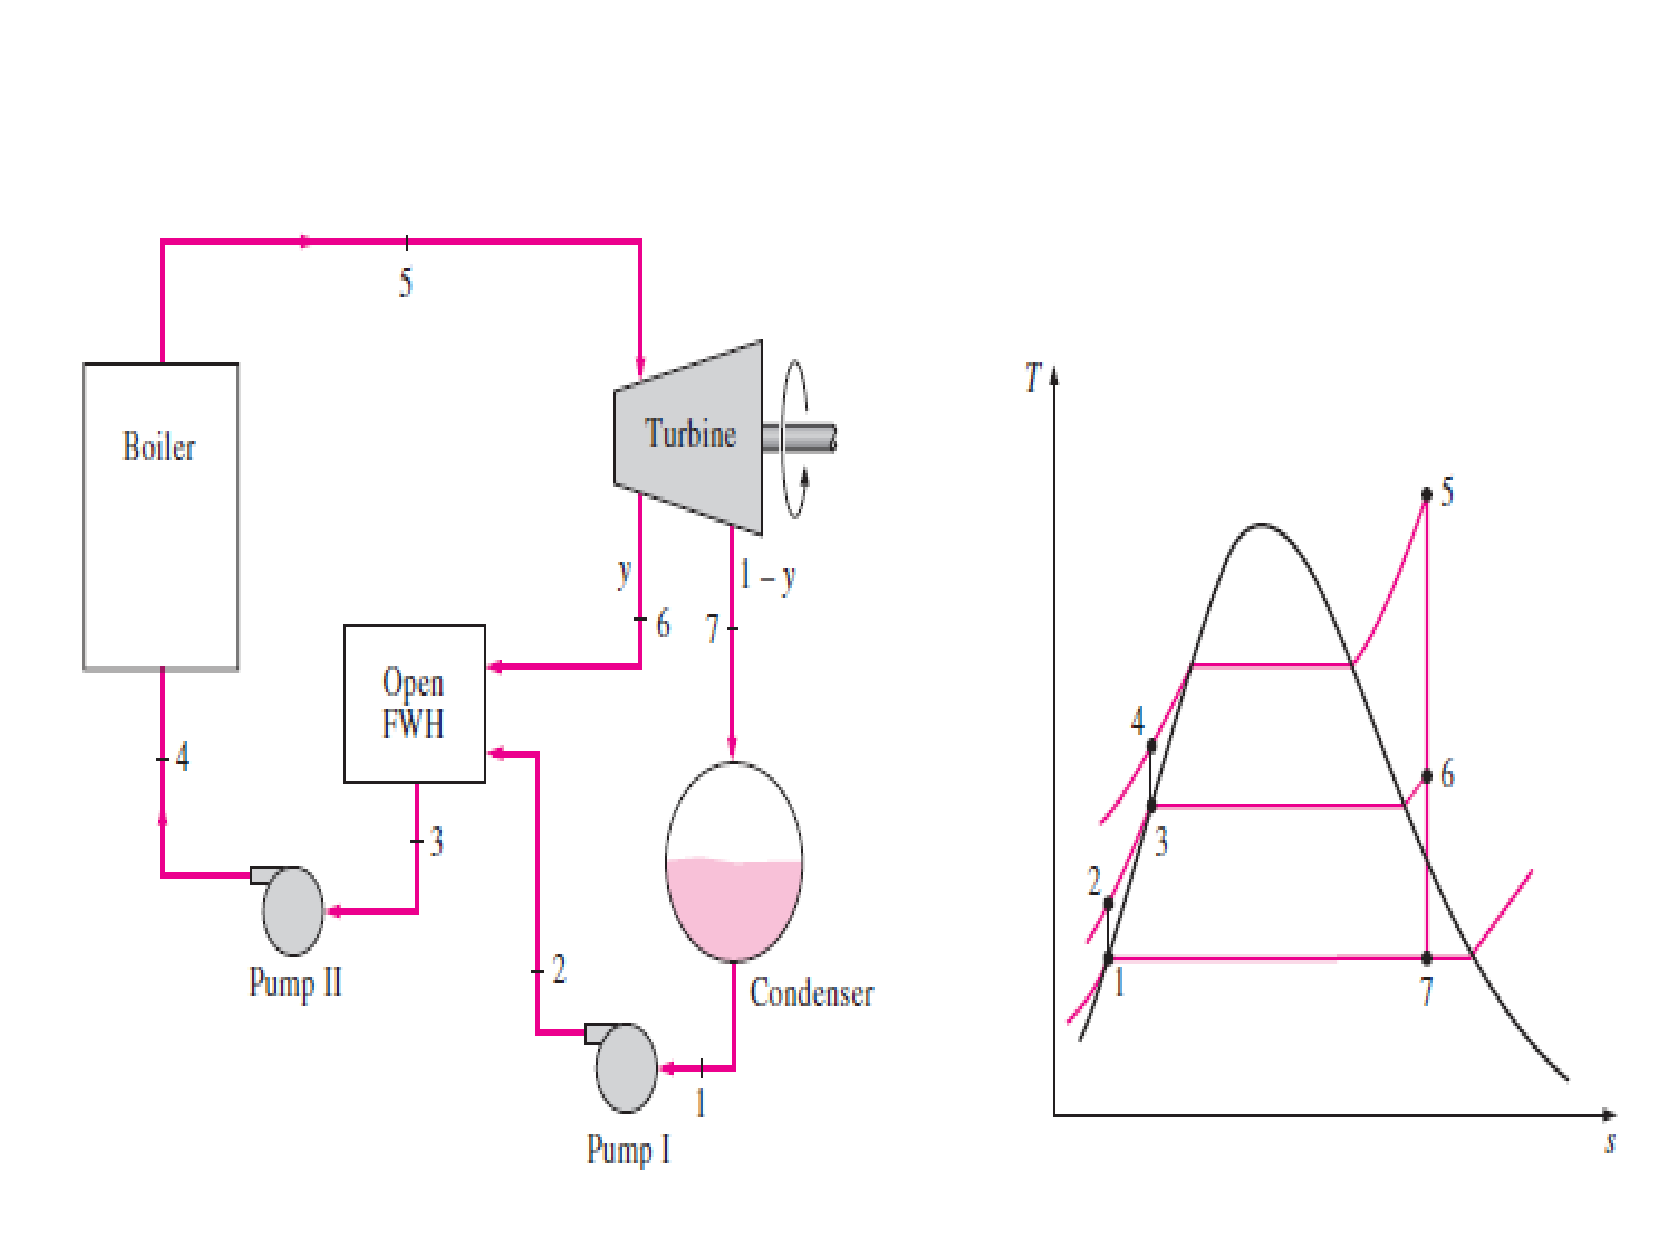
\includegraphics[width=6.25cm,clip]{./Pics/Regenerative_Rankine_Cycle_OpenFWH}
      \caption{\scriptsize Open feedwater heater.} 
     \end{center}
    \end{figure}  
   \end{column}
  \end{columns}
 \normalsize
\end{frame}



%%%
%%% Slide
%%%
\begin{frame}
 \frametitle{Ideal Regenerative Rankine Cycle}
  \begin{columns}
   \begin{column}[c]{0.5\linewidth}
    \begin{enumerate} %\scriptsize
     %\item <1-> In simple Rankine cycle the temperature of the working fluid entering the boiler is substantially lower than the boiler steam exiting temperature.  This results in lower thermal efficiency;
     %\item <2-> In the {\it Regenerative Rankine Cycle} the temperature of the fluid leaving the pump ({\it feedwater}) is raised in several stages using steam extracted from the turbine;
     %\item <3-> The device where the feedwater is heated by regeneration is called a {\it regenerator}, or a {\it feedwater heater (FWH)};
     \item <1-> Not only improve thermal efficiency but also deaerates the feedwater that helps prevent corrosion and pump cavitation;
     \item <2-> A FWH is a heat exchanger where heat is transferred from the steam to the feedwater either by mixing the two fluid streams ({\it open feedwater heaters}) or without mixing them ({\it closed feedwater heaters}).
    \end{enumerate} 
   \end{column}

   \begin{column}[c]{0.5\linewidth} 
    \begin{figure}%
     \begin{center}
      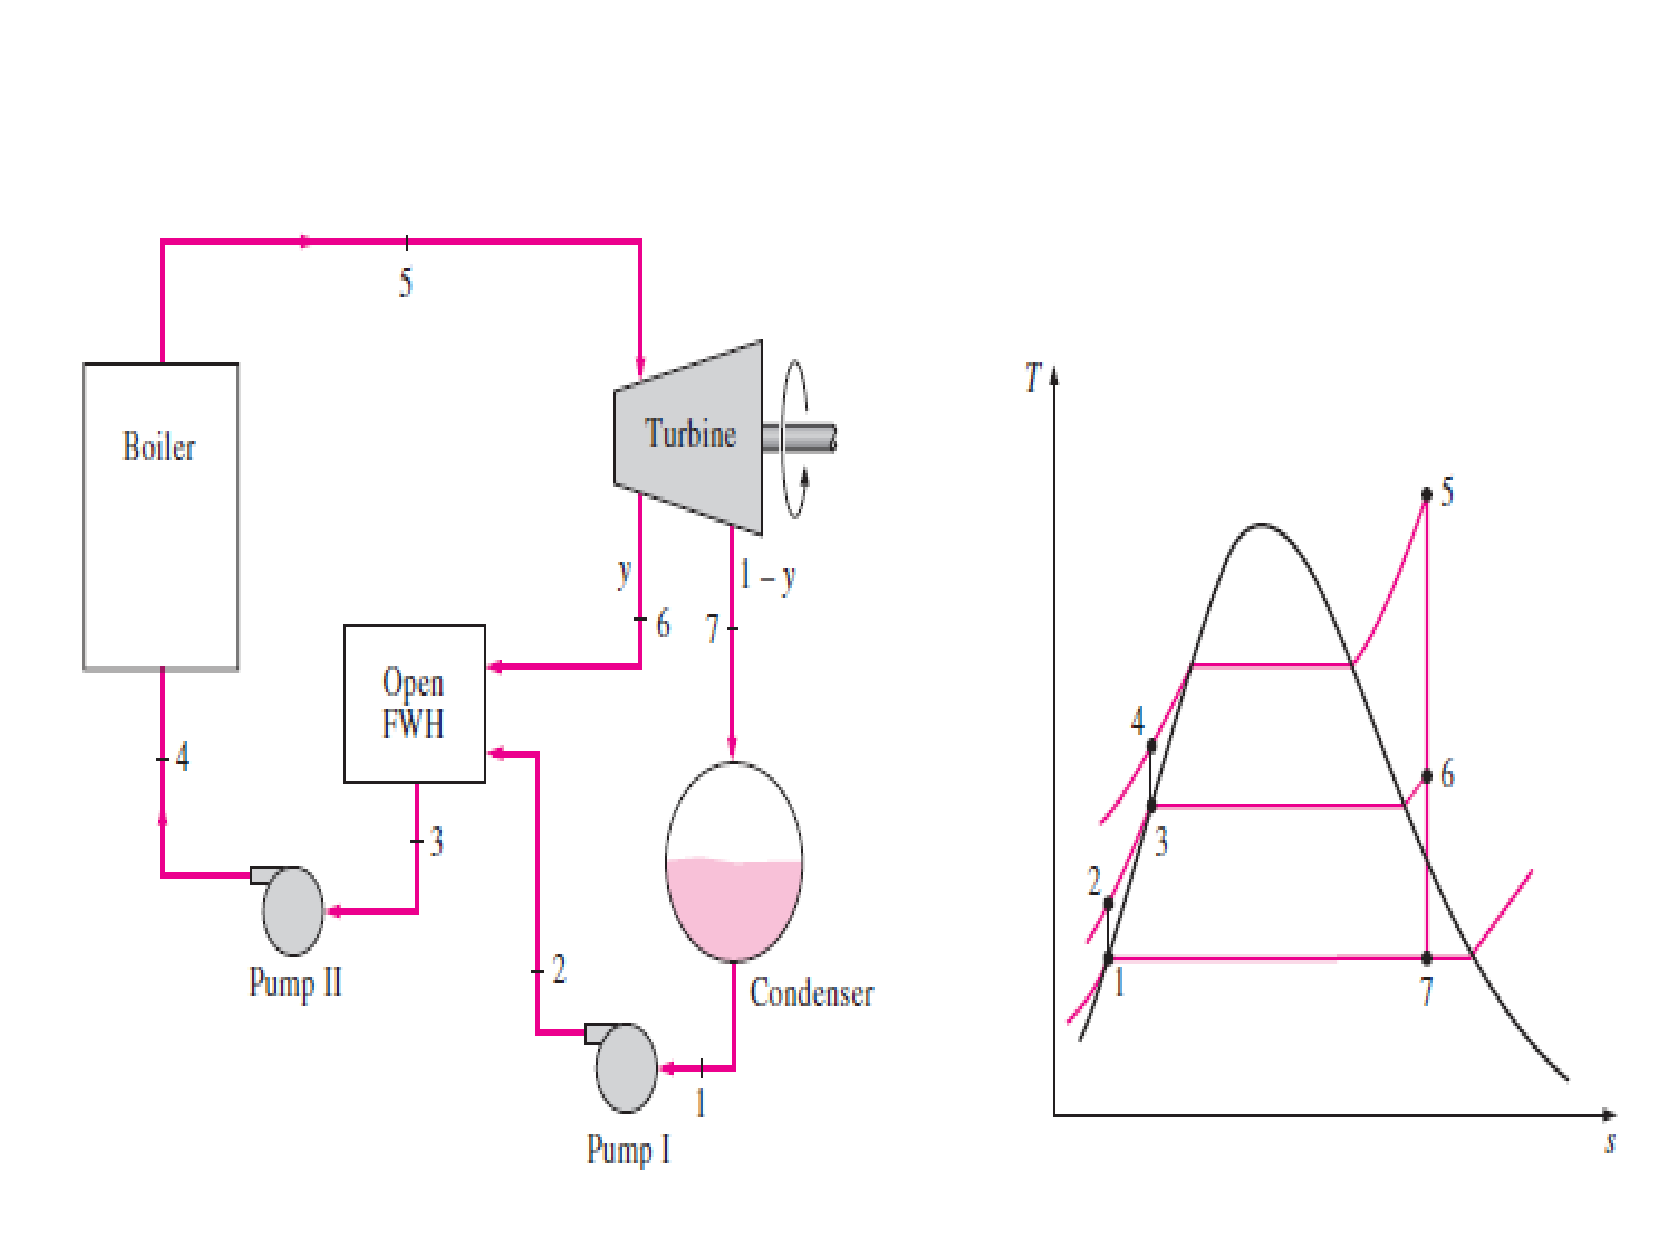
\includegraphics[width=6.25cm,clip]{./Pics/Regenerative_Rankine_Cycle_OpenFWH}
      \caption{\scriptsize Open feedwater heater.} 
     \end{center}
    \end{figure}  
   \end{column}
  \end{columns}
 \normalsize
\end{frame}



%%%
%%% Slide
%%%
\begin{frame}
 \frametitle{Ideal Regenerative Rankine Cycle}

  \begin{columns}
   \begin{column}[c]{0.5\linewidth}
    \begin{enumerate} %\scriptsize
     \item <1-> In Open FWH, steam is expanded isentropically in the turbine from a boiler pressure to an intermediate pressure;
     \item <2-> Part of the steam is then extracted and diverted to the FWH, whereas the remaining steam continues to expand isentropically to the condenser pressure;
      \item <3-> Steam leaves the condenser as a {\it saturated liquid} at the condenser pressure; 
      \item <4-> Feedwater enters the (isentropic) pump and is compressed to the FWH pressure and routed to the FWH where it is mixed with the steam extracted from the turbine;
      %\item <5->  A fraction of the steam extracted from the turbine ($y$) leaves the FWH as a {\it saturated liquid} $\left(P_{\text{FWH}}\right)$, and a second pump raises the pressure to $P_{\text{boiler}}$;
      %\item <6-> Heat added/extracted in the cycle (as shown in Fig.) is \textcolor{blue}{$q_{\text{in}}=h_{5}-h_{4}$} and \textcolor{blue}{$q_{\text{out}}=\left(1-y\right)\left(h_{7}-h_{1}\right)$};
      %\item <7-> Pump and turbine work is \textcolor{blue}{$W_{\text{turb}}^{\text{out}}=\left(h_{5}-h_{6}\right)+\left(1-y\right)\left(h_{6}-h_{7}\right)$} and \textcolor{blue}{$W_{\text{pump}}^{\text{in}}=\left(1-y\right)W_{\text{pump,1}}^{\text{in}}+W_{\text{pump,2}}^{\text{in}}$}
    \end{enumerate} 
   \end{column}

   \begin{column}[c]{0.5\linewidth} 
     \begin{figure}%
     \begin{center}
      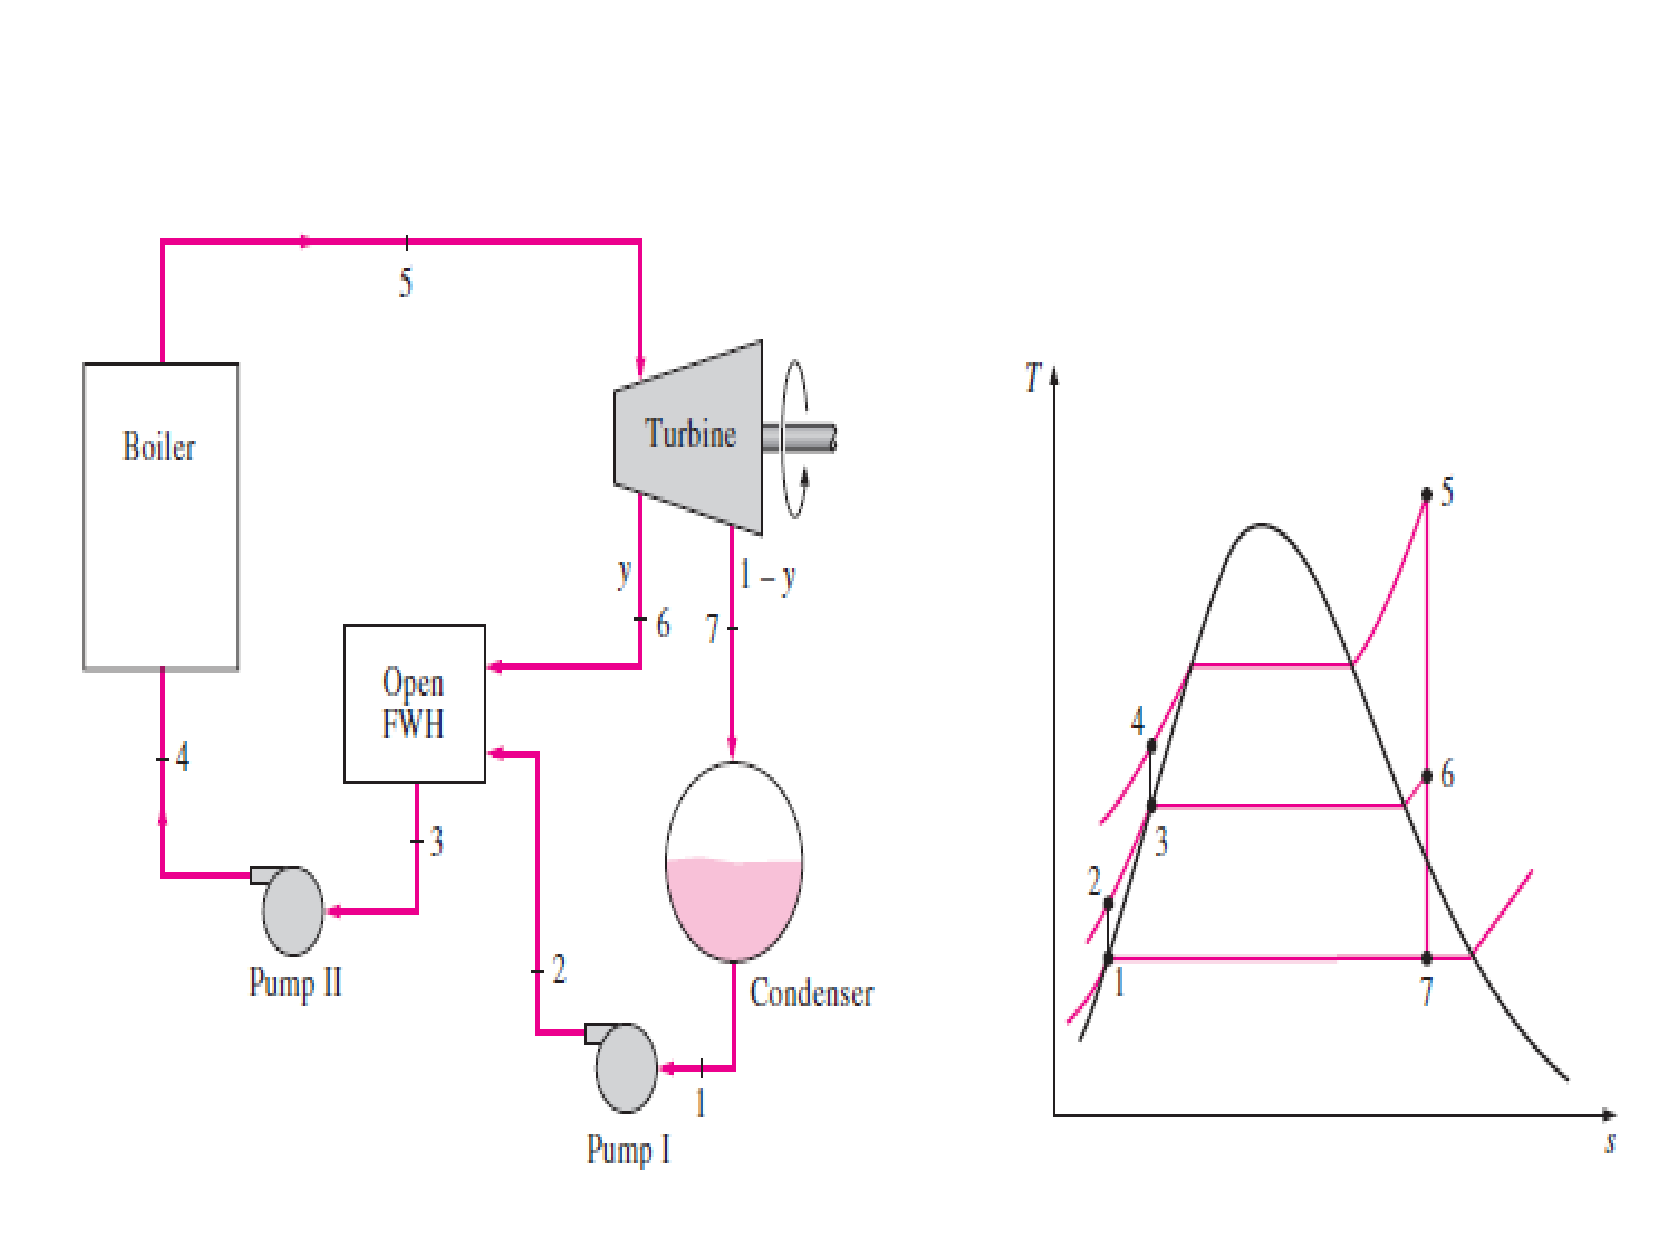
\includegraphics[width=6.25cm,clip]{./Pics/Regenerative_Rankine_Cycle_OpenFWH}
      \caption{\scriptsize Open feedwater heater.} 
     \end{center}
    \end{figure}  
   \end{column}
  \end{columns}
 \normalsize
\end{frame}



%%%
%%% Slide
%%%
\begin{frame}
 \frametitle{Ideal Regenerative Rankine Cycle}

  \begin{columns}
   \begin{column}[c]{0.5\linewidth}
    \begin{enumerate} %\scriptsize
     %\item %<1-> In Open FWH, steam is expanded isentropically in the turbine from a boiler pressure to an intermediate pressure;
     %\item %<2-> Part of the steam is then extracted and diverted to the FWH, whereas the remaining steam continues to expand isentropically to the condenser pressure;
     % \item %<3-> Steam leaves the condenser as a {\it saturated liquid} at the condenser pressure; 
     % \item %<4-> Feedwater enters the (isentropic) pump and is compressed to the FWH pressure and routed to the FWH where it is mixed with the steam extracted from the turbine;
      \item <1->  A fraction of the steam extracted from the turbine ($y$) leaves the FWH as a {\it saturated liquid} $\left(P_{\text{FWH}}\right)$, and a second pump raises the pressure to $P_{\text{boiler}}$;
      \item <2-> Heat added/extracted in the cycle (as shown in Fig.) is \textcolor{blue}{$q_{\text{in}}=h_{5}-h_{4}$} and \textcolor{blue}{$q_{\text{out}}=\left(1-y\right)\left(h_{7}-h_{1}\right)$};
      \item <3-> Pump and turbine work are \\
\medskip
       \textcolor{blue}{$W_{\text{turb}}^{\text{out}}=\left(h_{5}-h_{6}\right)+\left(1-y\right)\left(h_{6}-h_{7}\right)$}  and \\
\medskip
       \textcolor{blue}{$W_{\text{pump}}^{\text{in}}=\left(1-y\right)W_{\text{pump,1}}^{\text{in}}+W_{\text{pump,2}}^{\text{in}}$}
    \end{enumerate} 
   \end{column}

   \begin{column}[c]{0.5\linewidth} 
     \begin{figure}%
     \begin{center}
      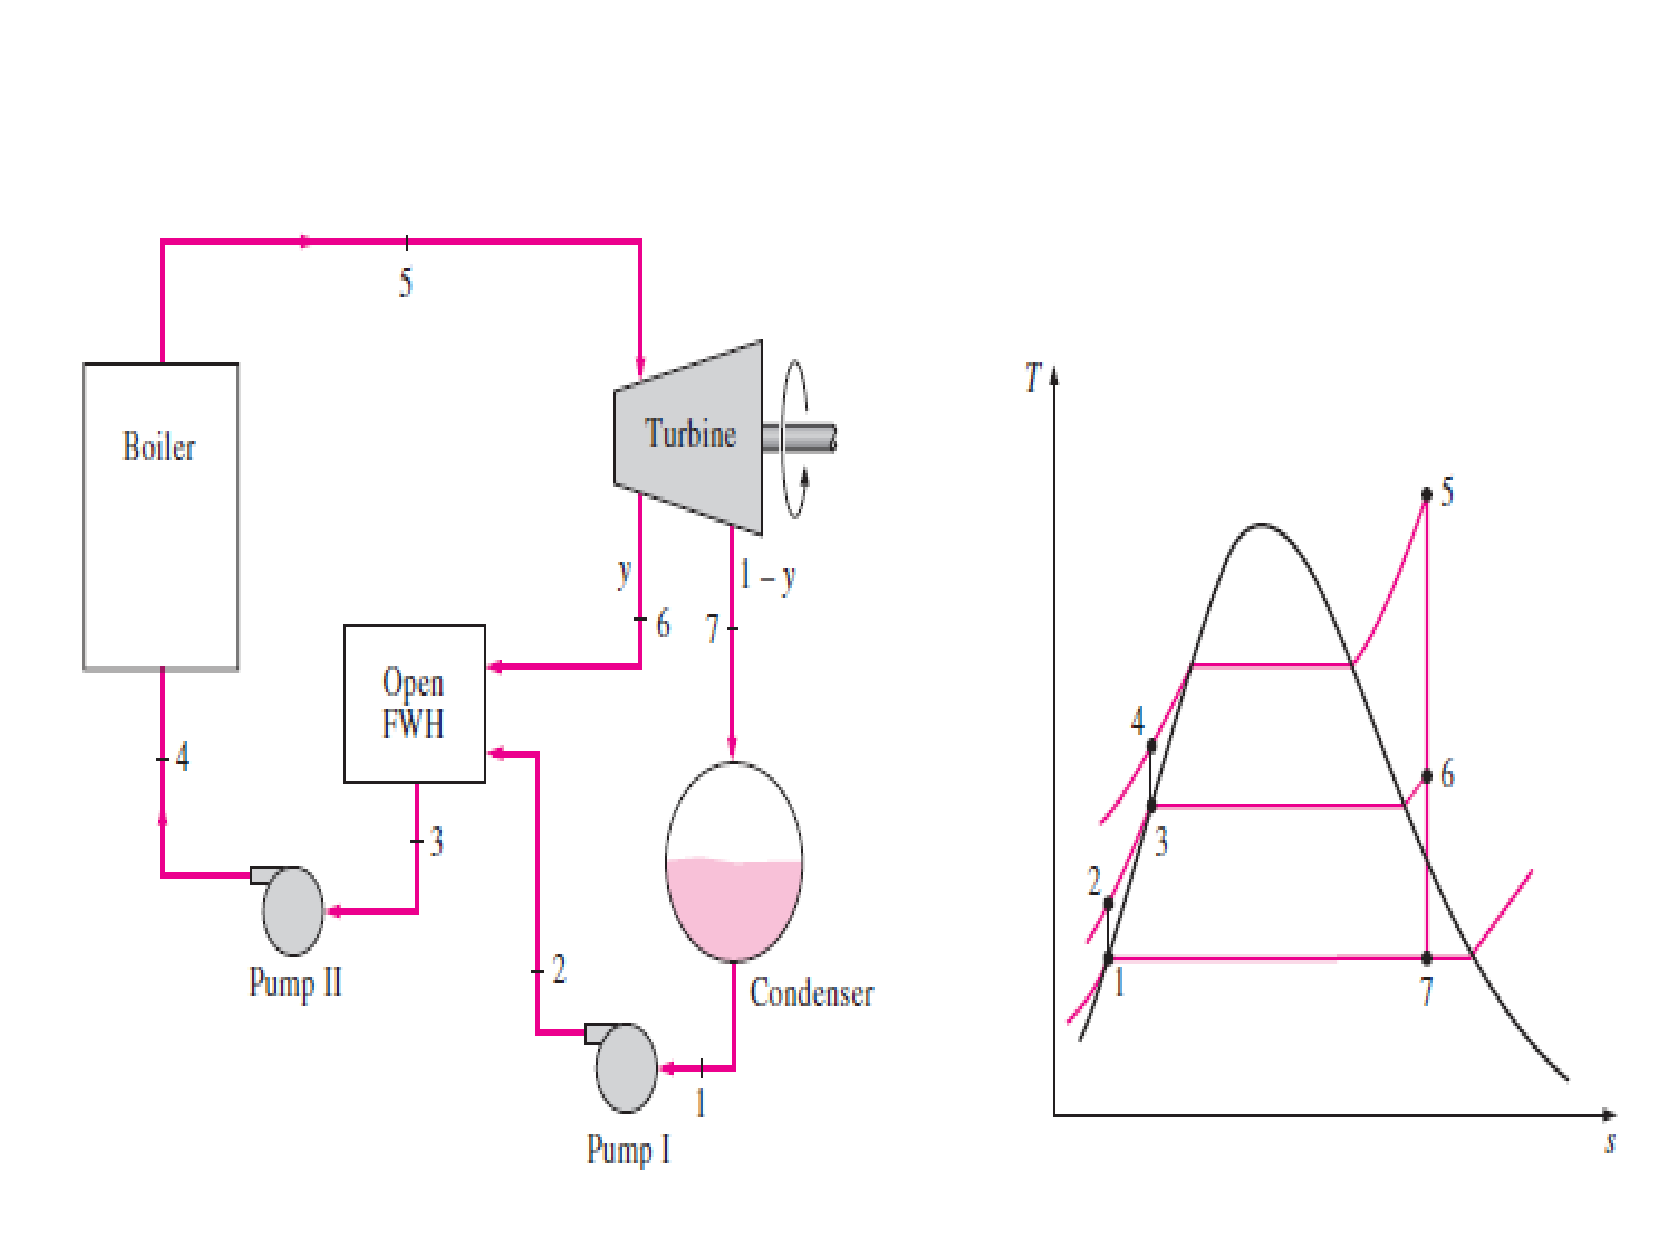
\includegraphics[width=6.25cm,clip]{./Pics/Regenerative_Rankine_Cycle_OpenFWH}
      \caption{\scriptsize Open feedwater heater.} 
     \end{center}
    \end{figure}  
   \end{column}
  \end{columns}
 \normalsize
\end{frame}



%%%
%%% Slide
%%%
\begin{frame}
 \frametitle{Ideal Regenerative Rankine Cycle}
    \begin{figure}%
     \begin{center}
      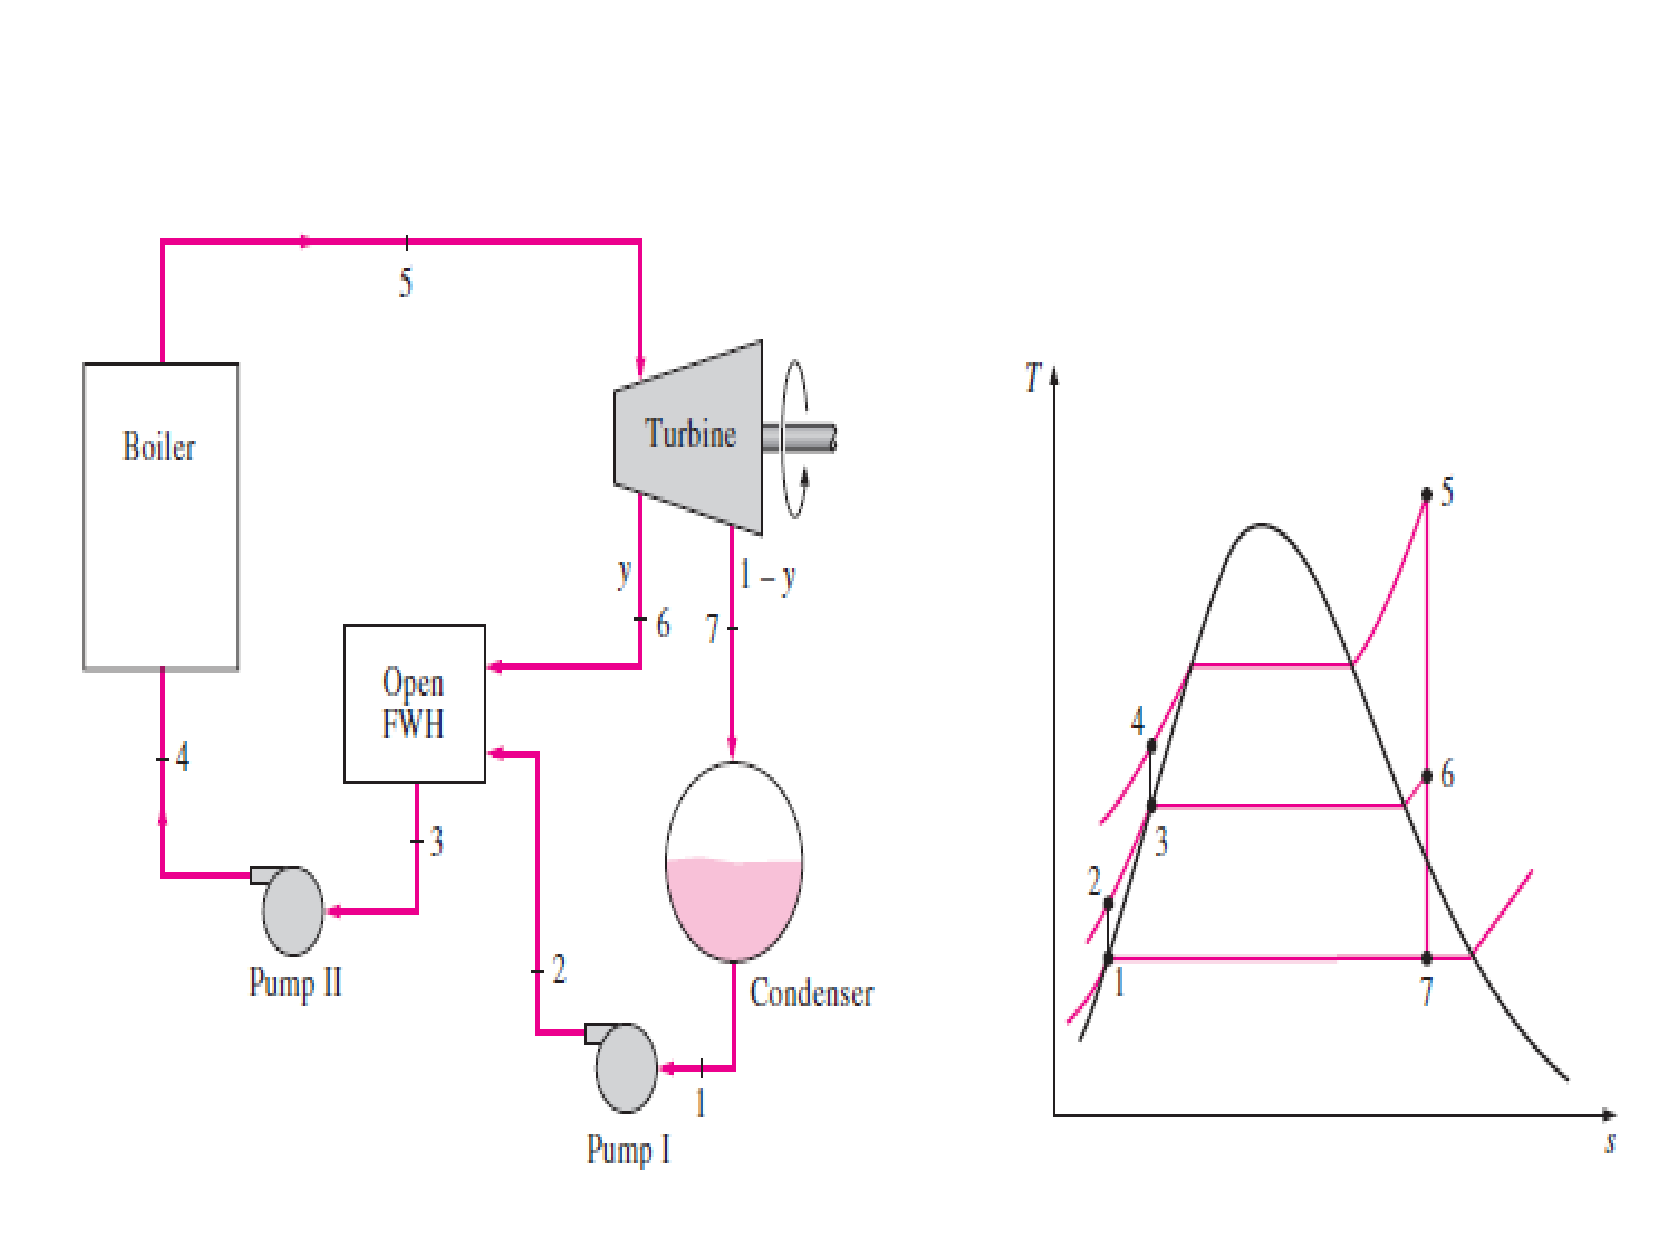
\includegraphics[width=6.25cm,clip]{./Pics/Regenerative_Rankine_Cycle_OpenFWH}
      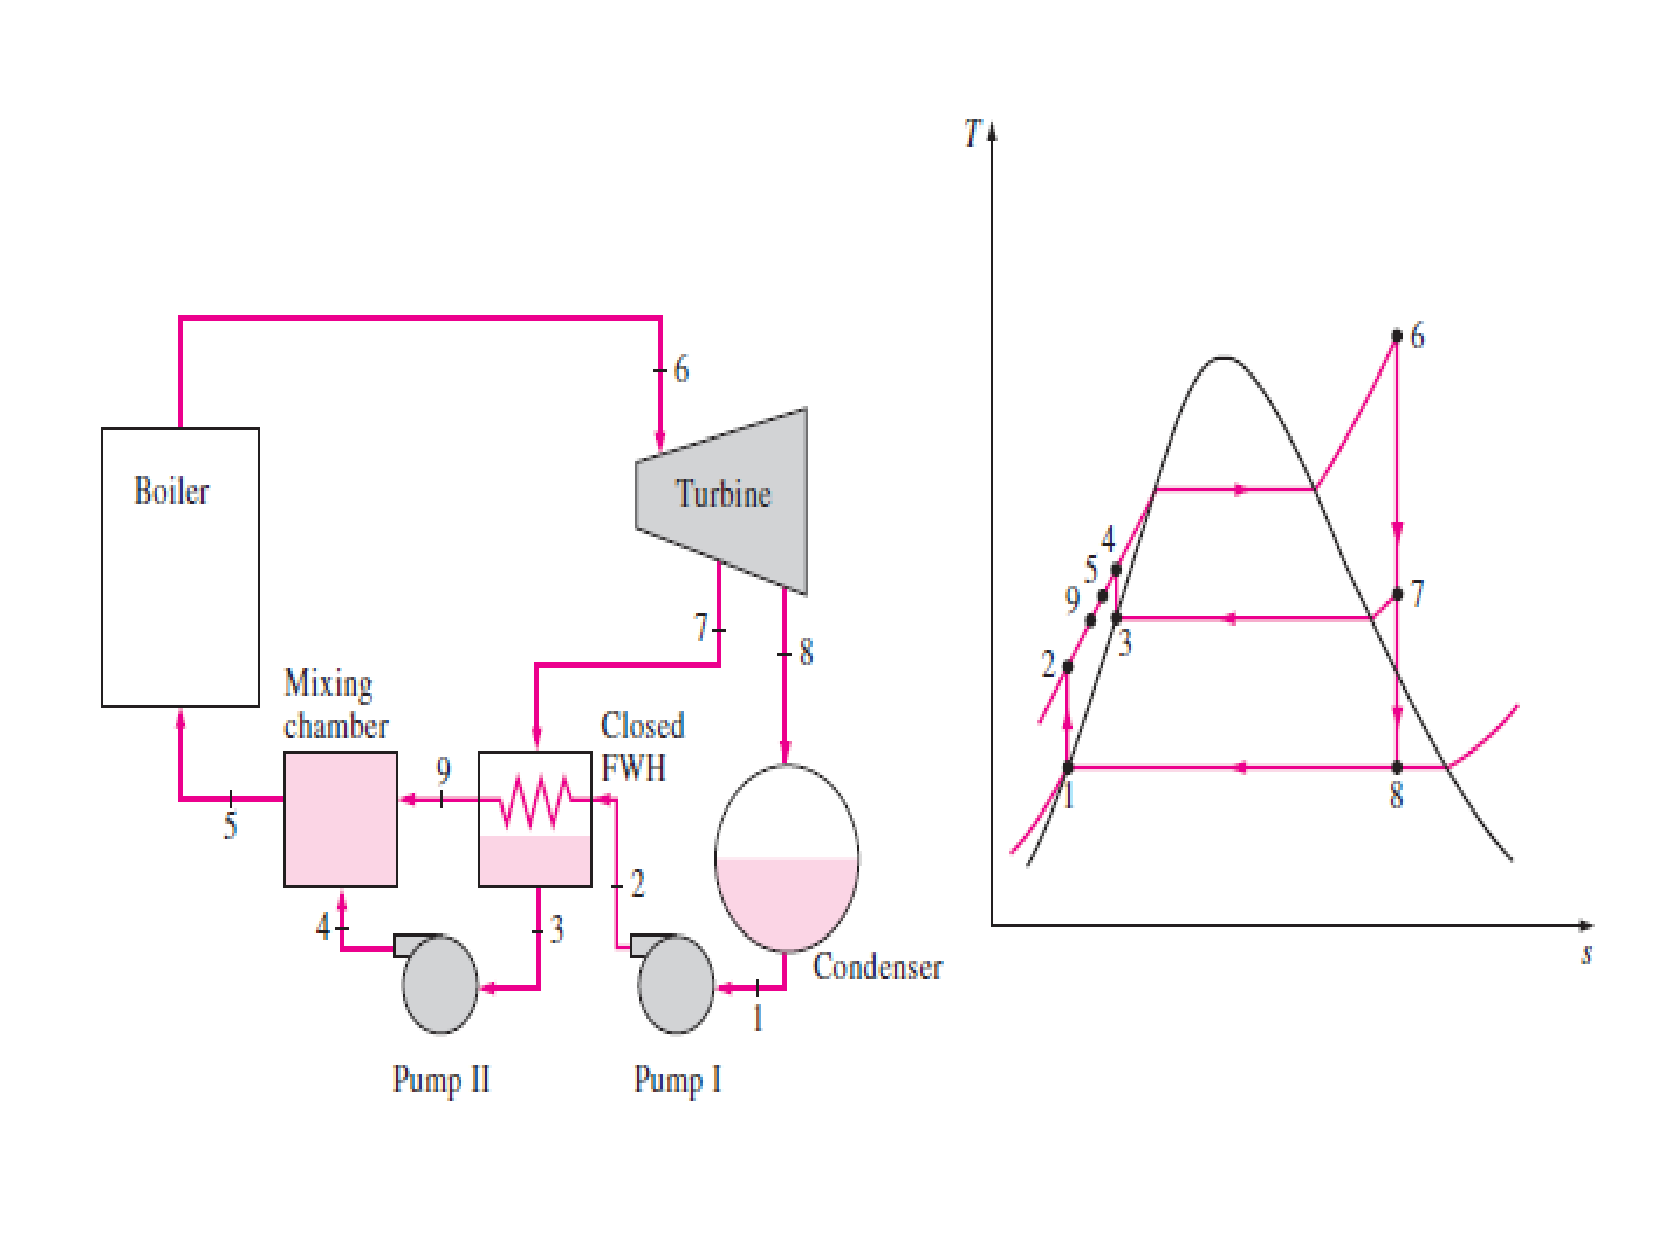
\includegraphics[width=6.25cm,clip]{./Pics/Regenerative_Rankine_Cycle_ClosedFWH}
\caption{Open and closed (rhs) Feedwater Heaters.}
     \end{center}
    \end{figure}  
\end{frame}


%%%
%%% Slide
%%%
\begin{frame}
 \frametitle{Ideal Regenerative Rankine Cycle}
  \begin{columns}
   \begin{column}[c]{0.5\linewidth}
    \begin{itemize}
     \item <1-> Advantages of Regenerative cycle over Simple Rankine Cycle
     \begin{enumerate} %\scriptsize
      \item <2-> The heating process in the boiler tends to become reversible;
      \item <3-> Thermal stresses in boiler are minimised due to the smaller temperature ranges in the boiler;
      \item <4-> Thermal efficiency is improved as the average temperature of heat addition to the cycle is increased;
      \item <5-> Due to continuous steam extraction, the content of moisture is reduced and this decreases the corrosion in the turbine;
      \item<6-> The size of the condenser is smaller (lower cost and better maintenance).
     \end{enumerate}
    \end{itemize} 
   \end{column}

   \begin{column}[c]{0.5\linewidth}  
    \begin{itemize}
     \item <7-> Disadvantages of Regenerative cycle over Simple Rankine Cycle
     \begin{enumerate} %\scriptsize
      \item <8-> Design of the power plant is more complex;
      \item <9-> As the number of heaters is increased, the greater maintenance (larger cost) is required;
      \item <10-> Heater are usually costly and the gain in thermal efficiency may not be enough. 
     \end{enumerate}
    \end{itemize} 
   \end{column}
  \end{columns}
  
\end{frame}


\section{Summary}
%%%
%%% Slide
%%%
\begin{frame}
 \frametitle{Summary}
  \begin{itemize}
   \item <1-> Components of vapour power cycles;
   \item <2-> Carnot cycle -- maximum possible efficiency derived from the Second Law of Thermodynamics;
   \item <3-> Rankine cycle is currently used in a number of industrial applications to transform thermal to mechanical/electrical energy;
   \item <4-> Practical improvements to the Rankine cycle to enhance thermal effciency.
  \end{itemize}
\end{frame}






\end{document}
